% !TeX spellcheck = en_GB

\newglossaryentry{pseudoinverse}
{name={pseudoinversa},
  description={La \index{pseudoinversa} pseudoinversa di Moore–Penrose $\mA^{+}$ 
 di una matrice $\mA \in \mathbb{R}^{\samplesize \times \nrfeatures}$ generalizza il 
 concetto di \gls{inverse} \cite{GolubVanLoanBook}. La pseudoinversa emerge in modo naturale 
 nell’ambito della \gls{ridgeregression} quando applicata ad un \gls{dataset} con \glspl{label} arbitrarie $\vy$ 
 e \gls{featuremtx} $\mX = \mA$ \cite[Ch.\ 3]{hastie01statisticallearning}. I \gls{modelparams} 
 appresi mediante \gls{ridgeregression} 
  sono dati da
  	\[
  	\widehat{\vw}^{(\regparam)}  = \big(\mA^T \mA + \regparam \mI \big)^{-1} \mA^\top \vy, \quad \regparam > 0.
  	\]
  	Possiamo quindi definire la pseudoinversa  $\mA^+ \in \mathbb{R}^{\nrfeatures \times \samplesize}$ tramite 
  	il limite \cite[Ch. 3]{benisrael2003generalized}
  	\[
  	\lim_{\regparam \to 0^+} \widehat{\vw}^{(\regparam)} = \mA^+ \vy.
  	\]
	},
 	first={pseudoinversa},
 	text={pseudoinversa}
 }
 

\newglossaryentry{inverse}
{name={matrice inversa},
 description={Una matrice inversa\index{matrice inversa} $\mA^{-1}$ è definita per una
 	matrice quadrata $\mA \in \mathbb{R}^{n \times n}$ a rango completo, cioè 
	le cui colonne sono linearmente indipendenti. In tal caso, si dice che $\mA$ è invertibile, 
	e la sua inversa soddisfa
 	\[
 	\mA \mA^{-1} = \mA^{-1} \mA = \mI.
 	\]  	
     Una matrice quadrata è invertibile se e solo se il suo\gls{det} è diverso da zero. Le matrici inverse 
     sono fondamentali nella risoluzione di sistemi di equazioni lineari e nella soluzione in forma chiusa della 
     \gls{linreg} \cite{Strang2007,Horn91}.  Il concetto di matrice inversa può essere esteso anche a matrici 
     non quadrate o non a rango pieno. Si può definire un' ``inversa sinistra'' $\mB$ 
     tale che $\mB \mA = \mI$, oppure un' ``inversa destra'' $\mC$ tale che $\mA \mC = \mI$. 
     Per matrici rettangolari o singolari in generale, la \gls{pseudoinverse} di Moore–Penrose
     $\mA^{+}$ fornisce un concetto unificato di matrice inversa generalizzata \cite{GolubVanLoanBook}.
 	 \begin{figure}
 		\centering
 		\begin{tikzpicture}[x=2cm,y=2cm]
 			% LEFT: Standard basis
 			\begin{scope}
 				\draw[->, thick] (0,0) -- (1,0) node[below right] {$\vx$};
 				\draw[->, thick] (0,0) -- (0,1) node[above left] {$\vy$};
 			\end{scope}
 			% CENTER: Transformed basis (by A)
 			\begin{scope}[shift={(2.0,0)}]
 				\coordinate (A) at (1.5,0.5);
 				\coordinate (B) at (-0.2,1.2);
				\draw[->, very thick, red] (0,0) -- (A) node[pos=0.5, below right] {$\mA \vx$};
 				\draw[->, very thick, red] (0,0) -- (B) node[above right] {$\mA \vy$};
 			\end{scope}
 			% RIGHT: Inverse transformation
 			\begin{scope}[shift={(4.9,0)}]
 				\draw[->, very thick, blue] (0,0) -- (1,0) node[pos=0.5, below] {$\mA^{-1} (\mA \vx) = \vx$};
 				\draw[->, very thick, blue] (0,0) -- (0,1) node[above] {$\mA^{-1} (\mA \vy) = \vy$};
 			\end{scope}
 			% Curved arrows between stages
 			\draw[->, thick, bend left=20] (1.2,0.4) to node[above] {$\mA$} (1.8,0.4);
 			\draw[->, thick, bend left=20] (3.8,0.4) to node[below] {$\mA^{-1}$} (4.4,0.4);
 		\end{tikzpicture}
 		\caption{Una matrice $\mathbf{A}$ rappresenta una trasformazione lineare di $\mathbb{R}^{2}$. La matrice inversa $\mathbf{A}^{-1}$ 
		rappresenta la trasformazione inversa. \label{fig_matrix_inverse_dict}} 
 	\end{figure}\\
	Si veda anche: \gls{det}, \gls{linreg}.},
  first={matrice inversa},
  text={matrice inversa}
}

\newglossaryentry{det}
{name={determinante},
 description={Il\index{determinante} determinante di una matrice quadrata $\mA\in\mathbb{R}^{n\times n}$, indicato con $\det(\mA)$, è l’unica funzione a valori scalari delle $n^2$ componenti di $\mA$ che soddisfa:
\begin{itemize}
  \item {\bf Multilinearità:} $\det$ è lineare in ciascuna colonna di $\mA$, mantenute fisse le altre.
  \item {\bf Antisimmetria:} lo scambio di due colonne di $\mA$ cambia il segno di $\det(\mA)$.
  \item {\bf Normalizzazione:} $\det(I_n)=1$, dove $I_n$ è la matrice identità $n\times n$.
\end{itemize}
Il determinante si calcola mediante lo sviluppo di Laplace rispetto alla riga $i$:
\[
  \det(\mA)
  = \sum_{j=1}^n (-1)^{i+j}\,a_{ij}\,\det(\mA_{ij}),
\]
dove $a_{ij}$ è l’elemento in posizione $(i,j)$ di $\mA$ e $\mA_{ij}$ è il minore ottenuto eliminando la riga $i$ e la colonna $j$.

Da un punto di vista geometrico, $\det(\mA)$ di una matrice quadrata 
 	$\mA \in \mathbb{R}^{n \times n}$ è uno scalare che caratterizza in che modo 
	l’applicazione di $\mA$ altera i volumi (e il loro orientamento) in $\mathbb{R}^n$ \cite{GolubVanLoanBook,Strang2007}. 
 	[Si osservi che una matrice $\mA$ rappresenta una trasformazione lineare su $\mathbb{R}^{n}$.] 
 	In particolare, se $\det(\mA) > 0$, l'orientazione viene preservata, se $\det(\mA) < 0$, l'orientazione viene invertita 
	mentre $\det(\mA) = 0$ implica un annullamento completo del volume, indicando che $\mA$ non è invertibile. 
 	Il determinante soddisfa inoltre la relazione $\det(\mA \mB) = \det(\mA) \cdot \det(\mB)$ e, se $\mA$ è 
 	diagonalizzabile con \glspl{eigenvalue} $\eigval{1}, \ldots, \eigval{n}$, allora $\det(\mA) = \prod_{i=1}^{n} \eigval{i}$ \cite{HornMatAnalysis}.
    Nei casi particolari $n=2$ (2D) e $n=3$ (3D), il determinante può essere interpretato rispettivamente come l’area o il volume orientati individuati dai vettori colonna di $\mA$.
    \begin{figure} 
    	\begin{center}
    \begin{tikzpicture}[x=2cm]
% LEFT: Standard basis vectors and unit square
	\begin{scope}
	\draw[->, thick] (0,0) -- (1,0) node[below right] {$\vx$};
	\draw[->, thick] (0,0) -- (0,1) node[above left] {$\vy$};
%	\draw[fill=gray!15] (0,0) -- (1,0) -- (1,1) -- (0,1) -- cycle;
	%\node at (0.5,0.5) {\small unit square};
	%\node at (0.5,-0.6) {standard basis};
	\end{scope}
% RIGHT: Transformed basis vectors and parallelogram
	\begin{scope}[shift={(2.8,0)}]
	\coordinate (A) at (1.5,0.5);
	\coordinate (B) at (-0.2,1.2);
	\draw[->, very thick, red] (0,0) -- (A) node[below right] {$\mA \vx$};
	\draw[->, very thick, red] (0,0) -- (B) node[above left] {$\mA \vy$};
	\draw[fill=red!20, opacity=0.6] (0,0) -- (A) -- ($(A)+(B)$) -- (B) -- cycle;
	\draw[dashed] (A) -- ($(A)+(B)$);
	\draw[dashed] (B) -- ($(A)+(B)$);
	\node at (0.8,0.6) {\small $\det(\mA)$};
	% Orientation arc
	\draw[->, thick, blue] (0.4,0.0) arc[start angle=0, end angle=35, radius=0.6];
%	\node[blue] at (0.25,1.25) {};
%	\node at (0.8,-0.6) {transformed basis};
	\end{scope}
% Arrow between plots
	\draw[->, thick] (1.3,0.5) -- (2.4,0.5) node[midway, above] {$\mA$};
	\end{tikzpicture}
	\end{center}
	\end{figure}
		\\ 
		Si veda anche: \gls{eigenvalue}, \gls{inverse}.
	},
	first={determinante},
	text={determinante}
}

\newglossaryentry{linearmap}{
	name={applicazione lineare},
	description={Un'\index{applicazione lineare} applicazione lineare $f: \mathbb{R}^n \rightarrow \mathbb{R}^m$ è una \gls{function} 
		che soddisfa l’additività:
		$f(\vx + \vy) = f(\vx) + f(\vy)$, e l’omogeneità:
		$f(c\vx) = c f(\vx)$ per tutti i vettori $\vx, \vy \in \mathbb{R}^n$ e per ogni scalare $c \in \mathbb{R}$. 
		In particolare, $f(\mathbf{0}) = \mathbf{0}$. Ogni applicazione lineare può essere rappresentata come una 
		moltiplicazione matriciale $f(\vx) = \mA \vx$, per qualche matrice $\mA \in \mathbb{R}^{m \times n}$. 
		L’insieme delle applicazioni lineari a valori reali per una data dimensione $n$ costituisce un \gls{linmodel} 
		che è impiegato in molti metodi di \gls{ml}. \\
		Si veda anche: \gls{linmodel}, \gls{linreg}, \gls{pca}, \gls{featurevec}.},
	first={applicazione lineare},
	text={applicazione lineare}
}


\newglossaryentry{vectorspace}
{name={spazio vettoriale},
	description={Uno\index{spazio vettoriale} spazio vettoriale (chiamato anche spazio lineare) è una 
	collezione di elementi (detti vettori) chiusa rispetto all'addizione vettoriale e alla moltiplicazione per uno scalare, ovvero,
		\begin{itemize}
			\item Se $\vx, \vy \in \mathcal{V}$, allora $\vx + \vy \in \mathcal{V}$.
			\item Se $\vx \in \mathcal{V}$ e $c \in \mathbb{R}$, allora $c \vx \in \mathcal{V}$.
			\item In particolare, $\mathbf{0} \in \mathcal{V}$.
		\end{itemize}
		Lo \gls{euclidspace} $\mathbb{R}^n$ è uno spazio vettoriale.
		I \glspl{linmodel} e le \glspl{linearmap} operano all'interno di tali spazi.\\
		Si veda anche: \gls{euclidspace}, \gls{linmodel}, \gls{linearmap}.},
	first={spazio vettoriale},
	text={spazio vettoriale}
}


\newglossaryentry{stochastic}
{name={stocastico},
	description={Un processo\index{stocastico} o un metodo si definisce stocastico se implica 
	una componente casuale oppure è governato da leggi probabilistiche. Nel \gls{ml}, i metodi 
	stocastici incorporano frequentemente elementi di casualità al fine di affrontare problematiche 
	come l'ottimizzazione (ad esempio, \gls{stochGD})
	o la modellazione dell' \gls{uncertainty} (ad esempio, \glspl{probmodel}). Un processo stocastico è una collezione
		di \glspl{rv} indicizzate nel tempo o nello spazio, utilizzate per modellare fenomeni aleatori 
		che evolvono nel tempo (ad esempio, il rumore nei segnali acquisiti dai sensori o le serie temporali finanziarie).\\
		Si veda anche:  \gls{ml}, \gls{stochGD}, \gls{uncertainty}, \gls{probmodel}, \gls{rv}, \gls{sbm}.},
	first={stocastico},
	text={stocastico}
}

\newglossaryentry{entropy}
{name={entropia},
	description={L'entropia quantifica l'\gls{uncertainty} o l’imprevedibilità associata ad una \gls{rv} \cite{coverthomas}. 
		Per una \gls{rv} discreta $x$ che assume valori in un insieme finito $\mathcal{S} = \{x_1, \ldots, x_n\}$ con 
		funzione di massa di probabilità $p_i \defeq \prob{x = x_i}$, l'entropia è definita come
		\[
		H(x) \defeq -\sum_{i=1}^n p_i \log p_i.
		\]
		L'entropia è massima quando tutti gli esiti sono equiprobabili, e minima (cioè nulla) quando l'esito è deterministico. 
		Una generalizzazione del concetto di entropia per le \glspl{rv} continue è l'\gls{diffentropy}. 
\\
		Si veda anche: \gls{uncertainty}, \gls{probmodel}.},
	first={entropia},
	text={entropia}
}

\newglossaryentry{diffentropy}
{name={entropia differenziale},
	description={Per\index{entropia differenziale} una \gls{rv} a valori reali $\featurevec \in \mathbb{R}^{\nrfeatures}$ 
		con \gls{pdf} $p(x)$,
		l'entropia differenziale è definita come \cite{coverthomas}
		\[
		h(\featurevec) \defeq - \int p(\featurevec) \log p(\featurevec) \, d\featurevec.
		\]
		L'entropia differenziale può assumere valori negativi e non possiede alcune proprietà dell'\gls{entropy} per 
		\glspl{rv} a valori discreti, come l'invarianza rispetto al cambiamento di variabili \cite{coverthomas}. 
		Tra tutte le \glspl{rv} con \gls{mean} $\meanvecgeneric$ e \gls{covmtx} $\covmtxgeneric$, 
		$h(\featurevec)$ è massima quando $\featurevec \sim \mvnormal{\meanvecgeneric}{\covmtxgeneric}$. 
		\\
		Si veda anche: \gls{uncertainty}, \gls{probmodel}.},
	first={entropia differenziale},
	text={entropia differenziale}
}


\newglossaryentry{minimum}
{
	name=minimo,
	description={Dato un insieme di numeri reali, il minimo\index{minimo} è il più piccolo tra questi.},
	first={minimo},text={minimo}
}

\newglossaryentry{function}
{name={funzione}, plural={funzioni}, 
	description={Una funzione\index{funzione} è una relazione   tra due insiemi $\mathcal{U}$ and $\mathcal{V}$ tale che ad ogni   
	elemento del primo insieme $u \in \mathcal{U}$ è associato un elemento del secondo insieme $v \in \mathcal{V}$ 
	\cite{RudinBookPrinciplesMatheAnalysis}. 
		  Si denota come $f: \mathcal{U} \rightarrow \mathcal{V}$, dove $\mathcal{U}$ è il dominio 
		  e $\mathcal{V}$ il codominio di $f$. In altri termini, una funzione $f$ definisce un valore unico 
		   $f(u) \in \mathcal{V}$ per ogni argomento $u \in \mathcal{U}$. 
	},
	first={funzione},
	text={funzione}
}


\newglossaryentry{map}
{name={mappa}, plural={mappe}, 
	description={Usiamo\index{mappa} il termine mappa come un 
	sinonimo di \gls{function}.
	\\
	Si veda anche: \gls{function}.
	},
	first={mappa},
	text={mappa}
}


\newglossaryentry{optproblem}
{name={problema di ottimizzazione}, 
	description={Un\index{problema di ottimizzazione} problema di ottimizzazione è una struttura 
		   matematica costituita da una \gls{objfunc} $f: \mathcal{U} \rightarrow \mathcal{V}$ 
		   definita su una variabile di ottimizzazione $\weights \in \mathcal{U}$, insieme ad un 
		   insieme ammissibile $\mathcal{W} \subseteq \mathcal{U}$. Si assume che il codominio $\mathcal{V}$  
		   sia ordinato, il che significa che, per ogni coppia di elementi $\mathbf{a}, \mathbf{b} \in \mathcal{V}$, 
		   sia possibile stabilire se $\mathbf{a} < \mathbf{b}$, $\mathbf{a} = \mathbf{b}$, 
		   oppure $\mathbf{a} > \mathbf{b}$. L’obiettivo dell’ottimizzazione è trovare quei valori  $\weights \in \mathcal{W}$ 
		   per cui la funzione obiettivo $f(\weights)$ risulta estrema —ovvero, minima or massima \cite{BoydConvexBook}, \cite{nesterov04}, \cite{BertsekasNonLinProgr}.
		   \\
		   Si veda anche: \gls{objfunc}.
	},
	first={problema di ottimizzazione},
	firstplural={problemi di ottimizzazione}, 
	plural={problemi di ottimizzazione}, 
	text={problema di ottimizzazione}
}

\newglossaryentry{optmethod}
{name={metodo di ottimizzazione},
	description={An\index{metodo di ottimizzazione} metodo di ottimizzazione è un \gls{algorithm} che 
		riceve in input una rappresentazione di un \gls{optproblem} e fornisce in output una soluzione (approssimata) 
		\cite{BoydConvexBook}, \cite{nesterov04}, \cite{BertsekasNonLinProgr}.
		 \\
		 Si veda anche: \gls{algorithm}, \gls{optproblem}.
	},
	first={metodo di ottimizzazione},
	firstplural={metodi di ottimizzazione}, 
	plural={metodi di ottimizzazione}, 
	text={metodo di ottimizzazione}
}

\newglossaryentry{fixedpointiter}
{name={iterazione funzionale},
	description={Un'\index{iterazione funzionale} iterazione funzionale è un metodo iterativo per la risoluzione 
		di un dato  \gls{optproblem}. Esso costruisce una successione $\weights^{(0)}, \weights^{(1)},\ldots$  
		 applicando ripetutamente un operatore $\fixedpointop$, ovvero, 
		 \begin{equation} 
		 	\label{equ_def_fixed_point_dict} 
		 	\weights^{(\iteridx+1)} = \fixedpointop \weights^{(\iteridx)} \mbox{, for } \iteridx=0,1,\ldots.
		 \end{equation} 
		 L'operatore $\fixedpointop$ è scelto in modo tale che ciascuno dei suoi punti fissi sia una soluzione 
		 $\widehat{\weights}$ del \gls{optproblem} considerato. Ad esempio, data una \gls{function} $f(\weights)$ 
		 \gls{differentiable} e \gls{convex}, i punti fissi dell'operatore $\fixedpointop: \weights \mapsto \weights - \nabla f(\weights)$ 
		 coincidono con i minimizzatori di $f(\weights)$. In generale, per un dato \gls{optproblem} con soluzione $\widehat{\weights}$, 
		 esistono molti operatori $\fixedpointop$ i cui punti fissi corrispondono a $\widehat{\weights}$. 
		 È evidente che si debba adottare un operatore $\fixedpointop$ in \eqref{equ_def_fixed_point_dict} che riduca la distanza dalla soluzione, in modo tale che
		\begin{equation} 
			\nonumber
			\underbrace{\normgeneric{ \weights^{(\iteridx+1)} - \widehat{\netparams}}{2}}_{\stackrel{\eqref{equ_def_fixed_point_dict}}{=} \normgeneric{ \fixedpointop \weights^{(\iteridx)} - \fixedpointop\widehat{\weights}}{2}}  \leq 	\normgeneric{ \weights^{(\iteridx)} - \widehat{\weights}}{2}. 
		\end{equation}
		Pertanto, si richiede che $\fixedpointop$ sia almeno non espansivo, ovvero che l'iterazione \eqref{equ_def_fixed_point_dict} 
		non produca \gls{modelparams} peggiori, nel senso di una maggiore distanza da una soluzione $\widehat{\weights}$. 
		Inoltre, ciascuna iterazione \eqref{equ_def_fixed_point_dict} dovrebbe anche comportare un certo progresso, 
		ovvero ridurre la distanza da una soluzione $\widehat{\weights}$. Questo requisito può essere formalizzato utilizzando 
		il concetto di \gls{contractop} \cite{Bauschke:2017}, \cite{fixedpoinIsta}. 
		L'operator $\fixedpointop$ è un \gls{contractop} se, per qualche $\contractfac \in [0,1)$,
		\begin{equation} 
			\nonumber
			\normgeneric{ \fixedpointop \weights\!-\!\fixedpointop \weights'}{2}  \leq  \contractfac	\normgeneric{\weights\!-\!\weights'}{2} \mbox{ holds for any } \weights,\weights'.
		\end{equation}
		Per un \gls{contractop} $\fixedpointop$, l'iterazione funzionale \eqref{equ_def_fixed_point_dict} genera 
		una successione $\weights^{(\iteridx)}$ che converge abbastanza rapidamente. In particolare \cite[Th. 9.23]{RudinBookPrinciplesMatheAnalysis}, 
		\begin{equation} 
			\nonumber
			\normgeneric{ \weights^{(\iteridx)} - \widehat{\weights}}{2} \leq \contractfac^{\iteridx} 	\normgeneric{ \weights^{(0)} - \widehat{\weights}}{2}. 
		\end{equation} 
		Qui, $\normgeneric{ \weights^{(0)} - \widehat{\weights}}{2}$ rappresenta la distanza tra 
		l’inizializzazione  $\weights^{(0)}$ e la soluzione $\widehat{\weights}$. 
		Si può dimostrare che per un'iterazione funzionale \eqref{equ_def_fixed_point_dict} con un operatore strettamente  
		non espansivo $\fixedpointop$ è garantita la convergenza ad un punto fisso di $\fixedpointop$ \cite[Cor. 5.16]{Bauschke:2017}. 
		La Figura \ref{fig_examples_nonexp_dict} mostra esempi di un operatore strettamente non espansivo, un operatore non espansivo, 
		ed un \gls{contractop}. Tutti questi operatori sono definiti nello spazio unidimensionale $\mathbb{R}$. 
		Un altro esempio di operatore strettamente non espansivo è l'\gls{proxop} of a \gls{function} \gls{convex}\cite{Bauschke:2017}, \cite{ProximalMethods}. 
		\definecolor{darkgreen}{rgb}{0.0, 0.5, 0.0}
		\begin{figure}[H]
			\begin{center} 
				\begin{tikzpicture}[scale=1.5]
					% Axes
					\draw[line width=1pt, ->] (-2,0) -- (2,0) node[right] {$\weight^{(\iteridx)}$};
					\draw[line width=1pt, ->] (0,-2) -- (0,2) node[above] {$\weight^{(\iteridx+1)}$};
					% Labels
					\node at (2.1,2.2) {$\fixedpointop^{(3)}$};
					\node at (1.9,-1.5) {$\fixedpointop^{(1)}$};
					\node at (1.5,1.2) {$\fixedpointop^{(2)}$};
					% Dashed lines at x=1 and y=1
					\draw[dashed] (1,-2) -- (1,2); % Vertical line at x=1
					\draw[dashed] (-2,1) -- (2,1); % Horizontal line at y=1
					\draw[dashed] (-2,-1) -- (2,-1); % Horizontal line at y=1
					\draw[dashed] (-1,-2) -- (-1,2); % Vertical line at x=1
					\node[above,xshift=4pt,yshift=-1pt] at (1,0) {$1$};
					\node[above,xshift=8pt,yshift=-1pt] at (0,-1) {$-1$};
					% First curve: y = 1/2 x + 1
					\draw[line width=2,domain=-2:2,smooth,blue] plot(\x,{0.5*\x + 1});
					% Second curve: y = -x
					\draw[line width=2,domain=-2:2,smooth,red] plot(\x,{-\x});
					% Third curve: y = x / |x| * min(|x|, 1)
					\draw[line width=2, domain=-2:-1,smooth,darkgreen] plot(\x,{-1});
					\draw[line width=2,domain=-1:1,smooth,darkgreen] plot(\x,{\x});
					\draw[line width=2,domain=1:2,smooth,darkgreen] plot(\x,{1});
				\end{tikzpicture}
			\end{center} 
			\caption{Esempio di un operatore non espansivo $\fixedpointop^{(1)}$, un operatore strettamente non espansivo $\fixedpointop^{(2)}$, e 
				un \gls{contractop} $\fixedpointop^{(3)}$. \label{fig_examples_nonexp_dict}}
		\end{figure} 
		Si veda anche: \gls{optproblem}, \gls{differentiable}, \gls{convex} \gls{function}, \gls{modelparams}, \gls{contractop}, \gls{proxop}.
	},
	first={iterazione funzionale},
	text={iterazione funzionale},
	firstplural={fiterazioni funzionale}, 
	plural={iterazioni funzionale}
}


\newglossaryentry{ergraph}
{name={grafo Erd\H{o}s-R\'enyi (grafo ER)},
	description={Un \gls{graph} ER è un \gls{probmodel} per \glspl{graph} definito su 
		su un dato insieme di nodi $\nodeidx=1,\ldots,\nrnodes$. Un modo per definire il \gls{graph} ER è 
		attraverso una collezione di \glspl{rv} binarie \gls{iid} $b^{(\edge{\nodeidx}{\nodeidx'})} \in \{0,1\}$, 
		per ciascuna coppia di nodi distinti $\nodeidx, \nodeidx'$. Una specifica \gls{realization}  
		di un \gls{graph} ER contiene un arco $\edge{\nodeidx}{\nodeidx'}$ se e solo se 
		$b^{(\edge{\nodeidx}{\nodeidx'})}=1$. Il \gls{graph} ER è parametrizzato dal 
		numero $\nrnodes$ di nodi e dalla \gls{probability} $\prob{b^{(\edge{\nodeidx}{\nodeidx'})}=1}$. 
		\\
		Si veda anche: \gls{graph}, \gls{probmodel}, \gls{iid}, \gls{rv}, \gls{realization}, \gls{probability}.
	},
	first={grafo Erd\H{o}s-R\'enyi (ER)},
	text={grafo ER}
}

\newglossaryentry{attack}
{name={attacco},  
	description={Un attacco\index{attacco} ad un sistema di \gls{ml} si riferisce ad un'azione intenzionale— 
		attiva o passiva—che compromette l'integrità, la disponibilità o la riservatezza del sistema.
		Gli attacchi attivi implicano la perturbazione di componenti quali i \glspl{dataset} (attraverso \gls{datapoisoning}) 
		o dei collegamenti di comunicazione tra i \glspl{device} in un contesto di \gls{fl}. Gli attacchi passivi, 
		come i \glspl{privattack}, mirano a estrarre \glspl{sensattr} senza modificare il sistema. 
		A seconda del loro obiettivo, si distinguono \glspl{dosattack}, attacchi \gls{backdoor} e \glspl{privattack}.
		\\
		Si veda anche:  \gls{datapoisoning}, \gls{privattack}, \gls{sensattr}, \gls{dosattack}, \gls{backdoor}.},
	plural={attacchi}, 
	first={attacco},
	firstplural={attacchi},
	text={attacco}
}

\newglossaryentry{privattack}
{name={attacco alla privacy},
	description={Un \gls{attack}\index{attacco alla privacy} alla privacy su un sistema di \gls{ml} mira a estrarre 
		\glspl{sensattr} degli individui sfruttando un accesso parziale a un \gls{model} di \gls{ml} addestrato. 
		Una delle forme di \gls{attack} alla privacy è l'\gls{modelinversion}.\\
		Si veda anche: \gls{attack}, \gls{sensattr}, \gls{modelinversion}, \gls{trustAI}, \gls{gdpr}.
		},
	plural={attacchi alla privacy}, 
	first={attacco alla privacy},
	firstplural={attacchi alla privacy}, 
	text={attacco alla privacy}
}

\newglossaryentry{epigraph}
{name={epigrafo},
  description={L'epigrafo\index{epigrafo} di una \gls{function} a valori reali $f : \mathbb{R}^n \to \mathbb{R} \cup \{+\infty\}$ 
  	è l'insieme dei punti che giacciono sul \gls{graph} della funzione o al di sopra di esso:
		\[
		\operatorname{epi}(f) = \left\{ (\mathbf{x}, t) \in \mathbb{R}^n \times \mathbb{R} \,\middle|\, f(\mathbf{x}) \leq t \right\}.
		\]
		Una \gls{function} è \gls{convex} se e solo se il suo epigrafo è un insieme \gls{convex} \cite{BoydConvexBook}, \cite{BertCvxAnalOpt}.
		\begin{figure}[H]
			\centering
			\begin{tikzpicture}[scale=1.0]
				\begin{axis}[
					axis lines = middle,
					xlabel = $x$,
					ylabel = {},
					xmin=-2, xmax=2,
					ymin=0, ymax=4.5,
					samples=100,
					domain=-1.5:1.5,
					thick,
					width=8cm,
					height=6cm,
					grid=none,
					axis on top,
					]
					% Function
					\addplot [blue, thick, domain=-1.5:1.5] {x^2} node [pos=0.85, anchor=south west, xshift=5pt] {$f(x)$};
					% Epigraph shading
					\addplot [
					name path=f,
					draw=none,
					ytick=\empty,
					domain=-1.5:1.5,
					] {x^2};
					\path[name path=top] (axis cs:-1.5,4) -- (axis cs:1.5,4);
					\addplot [
					blue!20,
					opacity=0.6,
					draw=none,
					] fill between [
					of=f and top,
					soft clip={domain=-1.5:1.5},
					];
					    \node[font=\small] at (axis cs:-1.0,2.3) {$\operatorname{epi} f$};
				%	\node[align=center, fill=white, draw=black, rounded corners, font=\small] at (axis cs:0.5,3.5) {Epigraph\\$\{(x,t) \mid f(x) \le t\}$};
				\end{axis}
			\end{tikzpicture}
			\caption{Epigrafo della \gls{function} $f(x) = x^2$ (ovvero la regione ombreggiata).}
		\end{figure}
		Si veda anche: \gls{function}, \gls{graph}, \gls{convex}.
	},
	first={epigrafo},
	text={epigrafo},
	plural={epigrafi}
}


\newglossaryentry{maximum}
{name=massimo,
 %description={Given a set of real numbers, the maximum\index{maximum} is the largest of those numbers.},
     description={Il massimo\index{massimo} di un insieme $\mathcal{A} \subseteq \mathbb{R}$ 
     	di numeri reali, qualora esista, è l’elemento più grande appartenente a tale insieme. Un insieme $\mathcal{A}$ 
     	ammette un massimo se è limitato superiormente e il suo \gls{supremum} appartiene ad $\mathcal{A}$ \cite[Sec.~1.4]{RudinBookPrinciplesMatheAnalysis}.
	\\ 
	Si veda anche: \gls{supremum}.},
 first={massimo},
 firstplural={massimi},
 plural={massimi},
 text={massimo}
}

\newglossaryentry{supremum}
{name=estremo superiore (o minimo dei maggioranti),
	description={L'estremo superiore\index{estremo superiore (o minimo dei maggioranti)} di un insieme di numeri reali è 
		è il più piccolo tra i numeri che sono maggiori o uguali ad ogni elemento dell'insieme. In termini più rigorosi, un 
		numero reale $a$ è l'estremo superiore di un insieme $\mathcal{A} \subseteq \mathbb{R}$ se: 1) $a$ 
		è un maggiorante di $\mathcal{A}$; e 2) nessun numero strettamente minore di $a$ è un maggiorante di $\mathcal{A}$. 
		Ogni insieme non vuoto di numeri reali che sia superiormente limitato ammette un supremo, 
		anche se questo non appartiene necessariamente all’insieme. \cite[Sec.~1.4]{RudinBookPrinciplesMatheAnalysis}.},
	firstplural={estremi superiori},
	plural={estremi superiori},
	first={estremo superiore (o minimo dei maggioranti)},
	text={estremo superiore}
}

\newglossaryentry{discrepancy}
{name=discrepanza,
	description={
		Si consideri\index{discrepancy} un'applicazione di \gls{fl} con \gls{netdata} 
		rappresentati da un \gls{empgraph}. I metodi di \gls{fl} impiegano una misura di discrepanza per  
		confrontare le funzioni \gls{hypothesis} dei \gls{localmodel} associati ai nodi $\nodeidx,\nodeidx'$ 
		connessi da un arco nel \gls{empgraph}.	
				\\ 
		Si veda anche: \gls{fl}, \gls{empgraph}, \gls{localmodel}.},
	first={discrepanza},
	firstplural={discrepanze}, 
  	plural={discrepanze}, 
	text={discrepanza}
}

\newglossaryentry{FedRelax}
{name={FedRelax},
	description={Un\index{FedRelax} \gls{distributedalgorithm} di \gls{fl}. 
		\\ 
		Si veda anche: \gls{fl}, \gls{distributedalgorithm}.},
	first={FedRelax},
	text={FedRelax}
} 

\newglossaryentry{fedavg}
{name={FedAvg},
	description={FedAvg\index{FedAvg} si riferisce ad una famiglia di \glspl{algorithm} iterativi di \gls{fl}. 
	Utilizza un'impostazione server-client e alterna fasi di addestramento dei \glspl{localmodel} 
	lato client, seguite dall'aggregazione dei \gls{modelparams} aggiornati sul server
	\cite{pmlr-v54-mcmahan17a}. L’aggiornamento locale presso il client $\nodeidx=1,\ldots,\nrnodes$ 
	al tempo $\iteridx$ parte dai \gls{modelparams} correnti $\weights^{(\iteridx)}$ forniti 
	dal server e consiste tipicamente nell'esecuzione di alcune iterazioni di \gls{stochGD}. Una volta completati gli aggiornamenti locali, essi vengono 
	aggregati dal server (ad esempio, facendo una media). La Figura \ref{fig_single_iteration_fedavg_dict} illustra l'esecuzione di una singola iterazione di FedAvg.
	\begin{figure}[H]
		\begin{center}
	\begin{tikzpicture}[>=Stealth, node distance=1cm and 1.5cm, every node/.style={font=\small}]
		% Styles
		\tikzstyle{server} = [circle, fill=black, minimum size=6pt, inner sep=0pt]
		\tikzstyle{client} = [circle, draw=black, minimum size=6pt, inner sep=0pt]
		% Time step labels
		\node (label1) at (0,3.5) {broadcast};
		\node[right=2.5cm of label1] (label2) {local update};
		\node[right=2.5cm of label2] (label3) {aggregate};
		% Time step k
		\node[server] (s1) at (label1 |- 0,2.5) {};
		\node[client] (c1l) at ($(s1) + (-1cm,-1cm)$) {};
		\node[client] (c1r) at ($(s1) + (1cm,-1cm)$) {};
		\node[] (dots1) at ($(s1) + (0cm,-1cm)$) {\ldots};
		\draw[->] (s1) -- (c1l) node[midway,left] {$\weights^{(\iteridx)}$};
		\draw[->] (s1) -- (c1r) node[midway,right] {$\weights^{(\iteridx)}$};
		\draw[->] (s1) -- (dots1);
		% Time step k+1 (local updates)
		\node[server] (s2) at (label2 |- 0,2.5) {};
		\node[client] (c2l) at ($(s2) + (-1cm,-1cm)$) {};
		\node[client] (c2r) at ($(s2) + (1cm,-1cm)$) {};
		\node[] (dots2) at ($(s2) + (0cm,-1cm)$) {\ldots};
		\node[below=0.2cm of c2l] {$\localparamsiter{\iteridx}{1}$};
		\node[below=0.2cm of c2r] {$\localparamsiter{\iteridx}{\nrnodes}$};
		% Time step k+2 (aggregation)
		\node[server] (s3) at (label3 |- 0,2.5) {};
			\node[above=0.01cm of s3, yshift=-4pt] {$\weights^{(\iteridx+1)}$};
		\node[client] (c3l) at ($(s3) + (-1cm,-1cm)$) {};
		\node[client] (c3r) at ($(s3) + (1cm,-1cm)$) {};
		\node[] (dots3) at ($(s3) + (0cm,-1cm)$) {\ldots};
		\draw[->] (c3l) -- (s3) node[midway,left] {$\localparamsiter{\iteridx}{1}$};
		\draw[->] (c3r) -- (s3)  node[midway,right] {$\localparamsiter{\iteridx}{\nrnodes}$};
		\draw[->] (dots3) -- (s3);
	\end{tikzpicture}
	\end{center}
		\caption{Illustrazione di una singola iterazione di FedAvg, che consiste nella trasmissione dei \gls{modelparams} da parte del server, 
		nell'esecuzione di aggiornamenti locali presso i client e nella loro aggregazione da parte del server. \label{fig_single_iteration_fedavg_dict}} 
	\end{figure} 
		Si veda anche: \gls{fl}, \gls{algorithm}, \gls{localmodel}, \gls{stochGD}.},
	first={FedAvg},
	text={FedAvg}
} 

\newglossaryentry{FedGD}
{name={FedGD},
	description={Un\index{FedGD} \gls{distributedalgorithm} di \gls{fl}che può essere implementato come propagazione di messaggi attraverso un \gls{empgraph}. 
		\\ 
		Si veda anche: \gls{fl}, \gls{distributedalgorithm}, \gls{empgraph}, \gls{gradstep}, \gls{gdmethods}.},
	first={FedGD},
	text={FedGD}
} 

\newglossaryentry{FedSGD}
{name={FedSGD},
	description={Un\index{FedSGD} \gls{distributedalgorithm} di \gls{fl} che può essere implementato come propagazione di messaggi attraverso un \gls{empgraph}. 
		\\ 
		Si veda anche: \gls{fl}, \gls{distributedalgorithm}, \gls{empgraph}, \gls{gradstep}, \gls{gdmethods}, \gls{stochGD}.},
	first={FedSGD},
	text={FedSGD}
} 

\newglossaryentry{hfl}
{name={federated learning orizzontale (FL orizzontale))},
description={\gls{fl} Orizzontale \index{federated learning orizzontale (FL orizzontale)} utilizza \gls{localdataset} costituiti da
	   \gls{datapoint} differenti, ma impiega lo stesso insieme di \gls{feature} per descriverli \cite{HFLChapter2020}.
		Ad esempio, nella previsione meteorologica si utilizza una rete di stazioni meteorologiche distribuite geograficamente, 
		ciascuna delle quali misura le medesime variabili, come la temperatura giornaliera, la pressione atmosferica e le precipitazioni,
		ma in regioni spazio-temporali differenti. Ogni regione rappresenta un \gls{datapoint} distinto, descritto attraverso lo stesso insieme di \gls{feature}.
		(ad esempio, la temperatura giornaliera o la pressione dell'aria).
		\\
		Si veda anche: \gls{ssl}, \gls{fl}, \gls{vfl}.},
	first={FL orizzontale},
	text={FL orizzontale}
} 

\newglossaryentry{dimred}
{name={riduzione della dimensionalità},
	description={Con riduzione della dimensionalità\index{riduzione della dimensionalità} ci si riferisce 
		a metodi che apprendono una trasformazione
		$\hypothesis: \mathbb{R}^{\nrfeatures} \rightarrow \mathbb{R}^{\nrfeatures'}$ 
		di un insieme (tipicamente ampio) di \glspl{feature} grezze$\feature_{1},\ldots,\feature_{\nrfeatures}$ 
		in un insieme più contenuto di \glspl{feature} significative $z_{1},\ldots,z_{\nrfeatures'}$. 
		L’utilizzo di un numero ridotto di \glspl{feature} comporta molteplici vantaggi: 
		\begin{itemize} 
			\item {Vantaggio statistico:} in genere si riduce il rischio di \gls{overfitting}, poiché la riduzione 
			del numero di \glspl{feature} comporta spesso una diminuzione della \gls{effdim} di un \gls{model}. 
			\item {Vantaggio computazionale:} un numero inferiore di \glspl{feature} implica un minor carico 
			computazionale durante l’addestramento dei \glspl{model} di \gls{ml}. Ad esempio, 
			i metodi di \gls{linreg} richiedono l’inversione di una matrice la cui dimensione dipende dal numero di \glspl{feature}.
			\item {\bf Visualizzazione:} la riduzione della dimensionalità riveste inoltre un ruolo essenziale nella visualizzazione 
			dei \gls{data}. Si può, ad esempio, apprendere una trasformazione che restituisce due \glspl{feature}  $z_{1},z_{2}$ 
			utilizzabili come coordinate in uno \gls{scatterplot}.La Fig.\ \ref{fig:dimred-scatter} 
			mostra lo \gls{scatterplot} di cifre scritte a mano posizionate secondo le \glspl{feature} trasformate. 
			In questo caso, i \glspl{datapoint} sono originariamente rappresentati da un ampio numero di valori in una scala di grigi (uno per ciascun pixel).
		\end{itemize} 
		 \begin{figure}[H]
		 \centering
		 \begin{tikzpicture}[scale=1]	
		% % Axes
		 	\draw[->] (-0.5,0) -- (5.5,0) node[right] {$z_1$};
		 	\draw[->] (0,-0.5) -- (0,4.5) node[above] {$z_2$};
		% % Example points with mini-images (can replace adjustbox with \includegraphics)
		 	\foreach \x/\y/\label in {
  		 		1.2/0.5/3,
  		 		0.8/2.0/8,
  		 		2.5/1.8/1,
  		 		3.8/3.5/6,
  		 		4.2/0.7/9,
  		 		2.8/3.0/7,
  		 		1.5/3.8/2
		 	}{
  		 		\node[draw, minimum size=0.6cm, inner sep=0pt] at (\x,\y)
    	 		{\label};
		 	}
		 	\end{tikzpicture}
		 	\caption{Esempio di riduzione della dimensionalità: dati di immagini ad alta dimensionalità
			(ad esempio, immagini ad alta risoluzione di cifre scritte a mano) proiettati in 2D utilizzando
			\glspl{feature} apprese $(z_1, z_2)$ e visualizzati in un \gls{scatterplot}.}
		 	\label{fig:dimred-scatter}
		 \end{figure}
		Si veda anche: \gls{overfitting}, \gls{effdim}, \gls{model}, \gls{scatterplot}.}, 
		 first={riduzione della dimensionalità},
		 text={riduzione della dimensionalità}
} 



\newglossaryentry{ml}
{name={machine learning (ML)},
		 description={Il ML\index{machine learning (ML)} ha come scopo la previsione 
	 una \gls{label} a partire dalle \gls{feature}s di un \gls{datapoint}. Le tecniche di ML raggiungono 
	 quest'obiettivo apprendendo una \gls{hypothesis} da uno \gls{hypospace} (o \gls{model}) 
	 mediante la minimizzazione di una \gls{lossfunc} \cite{MLBasics,HastieWainwrightBook}. 
	 Una precisa formulazione di questo principio è \gls{erm}. I metodi di ML si differenziano in base
	 a differenti scelte inerenti alla definizione dei \gls{datapoint}s (in termini di \gls{feature} e \gls{label}), 
	 alla struttura del \gls{model}, e alla specificazione della \gls{lossfunc} \cite[Ch. 3]{MLBasics}.
	 	 			\\ 
		Si veda anche: \gls{label}, \gls{feature}, \gls{datapoint}, \gls{hypothesis}, \gls{hypospace}, \gls{model}, \gls{lossfunc}, 
		\gls{erm}.},
	first={machine learning (ML)},
	text={ML}
} 


\newglossaryentry{featlearn}
{name={apprendimento delle caratteristiche},
	description={Si consideri un'applicazione di \gls{ml} con \glspl{datapoint} caratterizzati da 
		\glspl{feature} grezze $\featurevec \in \featurespace$. Con apprendimento delle \glspl{feature}\index{apprendimento delle caratteristiche} 
		ci si riferisce al processo di apprendimento di una \gls{map} 
		$$\featuremapvec: \featurespace \rightarrow \featurespace': \featurevec \mapsto \featurevec',$$ 
		che, a partire dalle \glspl{feature} grezze $\featurevec \in \featurespace$ di un \gls{datapoint}, restituisce nuove 
		\glspl{feature} $\featurevec' \in \featurespace'$ appartenenti ad un nuovo \gls{featurespace} $\featurespace'$. 
		Si ottengono diversi metodi di apprendimento delle \glspl{feature} in funzione delle diverse configurazioni 
		di $\featurespace,\featurespace'$,della definizione di uno \gls{hypospace} $\hypospace$ 
		di possibili \glspl{map} $\featuremapvec$, e di una misura quantitativa dell’utilità di uno specifico
		 $\featuremapvec \in \hypospace$. Ad esempio, \gls{pca} 
		utilizza $\featurespace \defeq \mathbb{R}^{\dimlocalmodel}$, $\featurespace' \defeq \mathbb{R}^{\dimlocalmodel'}$ 
		con $\dimlocalmodel' < \dimlocalmodel$, ed uno \gls{hypospace} 
		$$\hypospace\defeq \big\{ \featuremapvec: \mathbb{R}^{\dimlocalmodel}
		\!\rightarrow\! \mathbb{R}^{\dimlocalmodel'}\!:\!\featurevec'\!\defeq\!\mF \featurevec \mbox{ con qualche } \mF \!\in\! \mathbb{R}
		^{\dimlocalmodel' \times \dimlocalmodel} \big\}.$$ \Gls{pca} misura l'utilità di una specifica \gls{map} 
		$\featuremapvec(\featurevec)= \mF \featurevec$ 
	sulla base del \gls{minimum} errore di ricostruzione lineare ottenuto su un \gls{dataset} tale che 
$$ \min_{\mG \in \mathbb{R}^{\dimlocalmodel \times \dimlocalmodel'}} \sum_{\sampleidx=1}^{\samplesize} \normgeneric{\mG \mF \featurevec^{(\sampleidx)} - \featurevec^{(\sampleidx)}}{2}^{2}.$$ 
			\\ 
		Si veda anche: \gls{ml}, \gls{datapoint}, \gls{feature}, \gls{map}, \gls{featurespace}, \gls{hypospace}, \gls{pca}, \gls{minimum}, \gls{dataset}.}, 
	first={apprendimento delle caratteristiche},
	text={apprendimento delle caratteristiche}
} 

\newglossaryentry{autoencoder}
{name={autoencoder},
	description={Un autoencoder\index{autoencoder} è un metodo di \gls{ml} che apprende simultaneamente una \gls{map} di codifica
		$\hypothesis(\cdot) \in \hypospace$ e una \gls{map} di decodifica $\hypothesis^{*}(\cdot) \in \hypospace^{*}$. 
		Si tratta di un caso particolare di \gls{erm} in cui la \gls{loss} è calcolata a partire dall'errore di ricostruzione
		$\featurevec - \hypothesis^{*}\big(  \hypothesis \big( \featurevec \big) \big)$.
					\\ 
		Si veda anche: \gls{ml}, \gls{map}, \gls{erm}, \gls{loss}.},
	first={autoencoder},
	text={autoencoder}
} 

\newglossaryentry{vfl}
{name={federated learning verticale (FL verticale)},
	description={
		Il Federated Learning verticale\index{federated learning verticale (FL verticale)} si riferisce ad applicazioni di \gls{fl} 
		in cui i diversi \glspl{device} hanno accesso a differenti \glspl{feature} dello stesso insieme di
		\glspl{datapoint} \cite{VFLChapter}. 
		Formalmente, il \gls{dataset} globale considerato è
		\[
		\dataset^{(\mathrm{global})} \defeq \left\{ \left(\featurevec^{(1)}, \truelabel^{(1)}\right), \ldots, \left(\featurevec^{(\samplesize)}, \truelabel^{(\samplesize)}\right) \right\}.
		\]
		Indichiamo con $\featurevec^{(\sampleidx)} = \big( \feature^{(\sampleidx)}_{1}, \ldots, \feature^{(\sampleidx)}_{\nrfeatures'} \big)^{T}$, per $\sampleidx=1,\ldots,\samplesize$, 
	     	l'insieme completo di \glspl{featurevec} associati ai \glspl{datapoint}. Ogni \gls{device} $\nodeidx \in \nodes$ 
		osserva soltanto un sottoinsieme $\mathcal{F}^{(\nodeidx)} \subseteq \{1,\ldots,\nrfeatures'\}$ of \glspl{feature}, dando 
		luogo ad un \gls{localdataset} $\localdataset{\nodeidx}$ costituito da \glspl{featurevec}
		\[
		\featurevec^{(\nodeidx,\sampleidx)} = \big( \feature^{(\sampleidx)}_{\featureidx_{1}}, \ldots, \feature^{(\sampleidx)}_{\featureidx_{\nrfeatures}} \big)^{T}.
		\]
		Alcuni di questi \glspl{device} potrebbero avere anche accesso alle \glspl{label} $\truelabel^{(\sampleidx)}$, per $\sampleidx=1,\ldots,\samplesize$, 
		del \gls{dataset} globale. Una potenziale applicazione del FL verticale consiste nel facilitare la 
		collaborazione tra diversi fornitori di servizi sanitari. Ciascun fornitore raccoglie differenti tipologie di 
		misurazioni—come valori ematici, elettrocardiogrammi e radiografie polmonari—riferite agli stessi pazienti. 
		Un'altra applicazione riguarda un sistema nazionale di assicurazione sociale, in cui i dati sanitari, 
		gli indicatori finanziari, i comportamenti di consumo e i dati di mobilità sono raccolti da istituzioni differenti. 
		Il FL verticale consente un apprendimento congiunto tra queste entità, pur mantenendo livelli ben definiti di \gls{privprot}.		\begin{figure}[H]
			\begin{center}
			\begin{tikzpicture}[every node/.style={anchor=base}]
				  % --- Coordinate definitions ---
				\def\colX{0}
				\def\colY{1.6}
				\def\colZ{3.2}
				\def\colD{4.8}
				\def\colLabel{6.4} 
				\def\rowOne{0}
				\def\rowTwo{-1.2}
				\def\rowThree{-2.4}
				\def\rowFour{-3.6}
				% Manually place matrix entries
				\foreach \i/\label in {1/1, 2/2, 4/\samplesize} {
					\pgfmathsetmacro{\y}{-1.2*(\i-1)}
					\node (x\i1) at (0,\y) {$x^{(\label)}_{1}$};
					\node (x\i2) at (1.6,\y) {$x^{(\label)}_{2}$};
					\node (dots\i) at (3.2,\y) {$\cdots$};
					\node (x\i3) at (4.8,\y) {$x^{(\label)}_{\dimlocalmodel}$};
					\node (y\i) at (6.4,\y) {$\truelabel^{(\label)}$};
				}
				  % Outer rectangle for the full dataset
				\draw[dashed, rounded corners, thick]
				(-0.6,0.6) rectangle (6.9,-4.2);
				\node at (3.1,0.9) {$\dataset^{(\mathrm{global})} $};
			% Rectangle for local dataset 1 (e.g., first two features)
			\draw[dashed, rounded corners, thick]
			(-0.9,0.9) rectangle (2.1,-4.0);
			\node at (0.25,1.0) {$\localdataset{1}$};
		  	% --- Local dataset k (columns 2–3, rows 1–3) ---
			\draw[dashed, rounded corners, thick]
			($( \colZ + 1,,0.9 )$) rectangle
			($( \colLabel + 0.4, -4.5)$);
				\node at ($( \colZ + 0.9,-5 )$) {$\localdataset{\nodeidx}$};
			\end{tikzpicture}
			\end{center}
			\caption{Il FL verticale utilizza \glspl{localdataset} derivati dai \glspl{datapoint} di un \gls{dataset} globale comune. 
				I \glspl{localdataset} differiscono per la scelta delle \glspl{feature} utilizzate per caratterizzare i \glspl{datapoint}.
				\label{fig_vertical_FL_dict}}
		\end{figure}
		Si veda anche: \gls{fl}, \gls{privprot}.},
	first={federated learning verticale (FL verticale)},
	text={FL verticale}
} 

\newglossaryentry{interpretability}
 {name={interpretabilità},
 	description={Un metodo di \gls{ml} è interpretabile\index{interpretabilità}per un
	utente umano, se è in grado di comprendere il processo decisionale del metodo. 
	Un approccio per sviluppare una definizione precisa di interpretabilità tramite il concetto di simulabilità
	consiste nell’adottare proprio il concetto di simulabilità, ovvero la capacità di un essere umano di simulare 
	mentalmente il comportamento del \gls{model} 
	\cite{doshi2017towards,hase-bansal-2020-evaluating,Chen2018,Colin2022,Lipton2018}. 
 	L’idea è la seguente: se un utente umano comprende un metodo di \gls{ml}, allora dovrebbe
	essere in grado di anticiparne le \glspl{prediction} su di un \gls{testset}. Illustriamo
	un tale \gls{testset} nella Figura \ref{fig_aug_simulatability_dict} che mostra anche
	due \glspl{hypothesis} apprese, $\learnthypothesis$ e $\learnthypothesis'$. 
	Il metodi di \gls{ml} che produce l'\gls{hypothesis} $\learnthypothesis$ è interpretabile
	per un utente umano che abbia familiarità con il concetto di \gls{linearmap}. 
   	Poiché $\learnthypothesis$ corrisponde a una mappa lineare, l’utente può
	anticipare le \glspl{prediction} di $\learnthypothesis$ sul 
	\gls{testset}. Al contrario, il metodo di \gls{ml} che genera $\learnthypothesis'$ 
	non è interpretabile, poiché il suo comportamento non è più coerente con le aspettative dell’utente.
 	\begin{figure}
 		\begin{center} 
\begin{tikzpicture}[x=1.5cm, y=1cm]
  % Adjustable parameters
  \def\slope{0.4}
  \def\offset{2.0}
  % Axes
  \draw[->, very thick] (0,0.5) -- (7.7,0.5) node[below, xshift=-1cm] {$\feature$}; % x-axis
  \draw[->, very thick] (0.5,0) -- (0.5,4.2) node[above] {$\truelabel$};           % y-axis
  % Model line
  \draw[color=black, thick, dashed, domain=-0.5:7.2, variable=\x] 
    plot ({\x},{\slope*\x + \offset});
% non-interpretable model
  \draw[color=black, thick, dashed, domain=4:7.2, variable=\x] 
    plot ({\x},{\slope*\x + \offset-(\x-4)*0.5});
  \node[above] at (7.2, {\slope*7.2 + \offset}) {$\learnthypothesis(\feature)$};
  \node[above] at (7.2, {\slope*7.2 + \offset - 0.5*(7.2 - 4)}) {$\learnthypothesis'(\feature)$};
 %\node[above] at (7.2, {\slope*7.2 + \offset-(7.2-4)*0.3}) {$\learnthypothesis'(\feature)$};
  % Training Data points
  \foreach \x/\y/\c/\s in {
      1.2/1.0/blue/6, 1.4/1.0/blue/6, 1.7/1.0/blue/6,
      2.2/3.9/blue/12, 2.6/4.2/blue/12, 3.0/4.4/blue/12
  }{
    \coordinate (pt) at (\x,\y);
    \node[fill=\c, circle, draw, minimum size=\s pt, scale=0.6] at (pt) {};
    \draw[<->, >={Latex[width=2mm,length=4mm]}, color=\c, thick]
      (\x, {\slope*\x + \offset}) -- (pt);
  }
  % test set with pseudo-labels
    \foreach \x/\y/\c/\s in {
       5.7/2.6/red/12, 5.9/2.6/red/12, 6.2/2.6/red/12
   }{
     \coordinate (pt) at (\x,{\slope*\x + \offset});
     \node[fill=\c, circle, draw, minimum size=\s pt, scale=0.6] at (pt) {};
   }
  % Legend
  \draw[fill=blue] (4.2, 1.7) circle (0.1cm) node [black,xshift=0.2cm,anchor=west] {\gls{trainset} $\dataset$};
  \draw[fill=red]  (4.2, 1.2) circle (0.1cm) node [black,xshift=0.2cm,anchor=west] {\gls{testset} $\dataset'$};
\end{tikzpicture}
 		\caption{Possiamo valutare l'interpretabilità dei \glspl{model} di \gls{ml} addestrati, 
		$\learnthypothesis$ e $\learnthypothesis'$, confrontando le loro \glspl{prediction} 
		con le pseudo-\glspl{label} generate da un utente umano per $\dataset'$.
		\label{fig_aug_simulatability_dict}}
 		\end{center}
	 \end{figure} 
 	 Il concetto di interpretabilità è strettamente correllata al concetto di spiegabilità, 
 	 poiché entrambe mirano a rendere i metodi di \gls{ml} più comprensibili per gli esseri umani. 
	 Nel contesto della Figura \ref{fig_aug_simulatability_dict}, l'interpretabilità di un metodo di \gls{ml} 
	 $\learnthypothesis$ richiede che l’utente umano sia in grado di anticiparne le \glspl{prediction} 
	 su di un generico \gls{testset}. Questo si contrappone con la spiegabilità, in cui l’utente è supportato da spiegazioni esterne 
	 – come le saliency maps o esempi di riferimento tratti dal \gls{trainset} - 
	 per comprendere le predizioni $\learnthypothesis$ su uno specifico $\dataset'$. \\ 
	 Si veda anche: \gls{explainability}, \gls{trustAI}, \gls{regularization}, \gls{lime}.
},
 	first={interpretabilità},
 	text={interpretabilità}
 }
 
\newglossaryentry{multitask learning}
{name={apprendimento multitask},
	description={L'apprendimento multitask\index{apprendimento multitask} si propone di sfruttare le relazioni 
	tra differenti \glspl{learningtask}. Si considerino due \glspl{learningtask} ottenuti dallo  
	 	stesso \gls{dataset} di istantanee di una webcam. Il primo task consiste nel predire la presenza di un essere umano, 
		mentre il secondo ha l'obiettivo di predire la presenza di un'automobile. Una possibile strategia consiste nell'utilizzare 
		una struttura comune di \gls{deepnet} per entrambi i task, modificando esclusivamente i \gls{weights} dello strato di output finale.
	 			\\ 
		Si veda anche: \gls{learningtask}, \gls{dataset}, \gls{deepnet}, \gls{weights}.},
	first={apprendimento multitask},
	text={apprendimento multitask}
}

\newglossaryentry{learningtask}
{name={task di apprendimento}, 
	description={Si consideri \index{task di apprendimento} un \gls{dataset} $\dataset$ costituito da diversi \glspl{datapoint}, ognuno dei quali
	 	caratterizzato da un insieme di \glspl{feature} $\featurevec$. Ad esempio, il \gls{dataset} $\dataset$ 
	 	potrebbe essere costituito dalle immagini di un particolare database. Talvolta può risultare 
		utile rappresentare un \gls{dataset} $\dataset$, insieme alla scelta delle \glspl{feature}, attraverso una \gls{probdist} $p(\featurevec)$. 
	 	Un task di apprendimento associato a $\dataset$ consiste in una specifica  
	 	scelta per l'\gls{label} di un \gls{datapoint} e per il corrispondente \gls{labelspace}. 
	 	Data una scelta per la \gls{lossfunc} e per il \gls{model}, un task di apprendimento dà origine ad 
		un'istanza di \gls{erm}. Di conseguenza, è possibile definire un task di apprendimento anche tramite un'istanza di \gls{erm}, 
		ovvero attraverso una \gls{objfunc}. Si noti che, a partire dallo stesso \gls{dataset}, si possono ottenere task di apprendimento differenti 
	 	scegliendo diverse \glspl{feature} e \gls{label} per ciascun \gls{datapoint}. Questi  
	 	task di apprendimento sono correlati, in quanto basati sullo stesso \gls{dataset}, e risulta generalmente preferibile 
		risolverli in parallelo (tramite metodi di \gls{multitask learning}) piuttosto che affrontarli separatamente. \cite{Caruana:1997wk}, \cite{JungGaphLassoSPL}, \cite{CSGraphSelJournal}.
	 			\\ 
		Si veda anche: \gls{dataset}, \gls{datapoint}, \gls{feature}, \gls{probdist}, \gls{label}, \gls{labelspace}, \gls{lossfunc}, \gls{model}, \gls{erm}, \gls{objfunc}, \gls{multitask learning}.},
	first={task di apprendimento},
	text={task di apprendimento}
}

\newglossaryentry{explainability}
{name={spiegabilità},
	description={Definiamo\index{spiegabilità} la spiegabilità (soggettiva) di un metodo di \gls{ml}  
		come il livello di simulabilità \cite{Colin:2022aa} della \glspl{prediction} 
		fornite da un sistema di \gls{ml} ad un utente umano. Misure quantitative della 
		spiegabilità (soggettiva) di un \gls{model} addestrato possono essere costruite
		confrontando le sue \glspl{prediction} con le \glspl{prediction} fornite da un utente 
		su un \gls{testset} \cite{Colin:2022aa}, \cite{Zhang:2024aa}. In alternativa, è possibile utilizzare 
		\glspl{probmodel} per \gls{data} e misurare la spiegabilità di un \gls{model} di \gls{ml} 
		 attraverso l' \gls{entropy} condizionale (o differenziale) delle sue \glspl{prediction}, date le \glspl{prediction} dell'utente \cite{JunXML2020}, \cite{Chen2018}.
						\\ 
		Si veda anche: \gls{trustAI}, \gls{regularization}.
		},
		first={spiegabilità},
		text={spiegabilità}
	}
	
\newglossaryentry{lime}
{name={local interpretable model-agnostic explanations (LIME)},
	description={Si consideri\index{local interpretable model-agnostic explanations (LIME)} 
		un \gls{model} addestrato (o un'\gls{hypothesis} appresa) $\widehat{\hypothesis} \in \hypospace$, 
		che mappa il \gls{featurevec} di un \gls{datapoint} nella \gls{prediction} $\widehat{\truelabel}= \widehat{\hypothesis}$. 
		LIME (o Spiegazioni Locali Interpretabili e Agnostiche rispetto al Modello) è una tecnica per spiegare il comportamento 
		di $\widehat{\hypothesis}$ localmente, in prossimità di un \gls{datapoint} con \gls{featurevec} $\featurevec^{(0)}$ \cite{Ribeiro2016}. 
		La \gls{explanation} iene fornita sotto forma di un'approssimazione locale $g \in \hypospace'$ di $\widehat{\hypothesis}$ 
		(si veda la Figura \ref{fig_lime_dict}). Tale approssimazione può essere ottenuta mediante un'istanza di \gls{erm} 
		con un \gls{trainset} opportunamente costruito. In particolare, il \gls{trainset} è costituito da \glspl{datapoint} 
		il cui \gls{featurevec} $\featurevec$ è vicino a $\featurevec^{(0)}$ e con (pseudo-)\gls{label} $\widehat{\hypothesis}(\featurevec)$. 
		Si noti che è possibile utilizzare un \gls{model} $\hypospace'$ diverso da quello originale \gls{model} $\hypospace$ 
		per l'approssimazione; ad esempio, si può impiegare un \gls{decisiontree} per approssimare localmente una \gls{deepnet}. 
		Un'altra scelta molto comune per $\hypospace'$ è il \gls{linmodel}. 
		\begin{figure}[H]
		\begin{center}
		\begin{tikzpicture}
			\begin{axis}[
				axis lines=middle,
				xlabel={$\featurevec$},
				ylabel={$\truelabel$},
				xtick=\empty,
				ytick=\empty,
				xmin=0, xmax=6,
				ymin=0, ymax=6,
				domain=0:6,
				samples=100,
				width=10cm,
				height=6cm,
				clip=false
			]
			  % Non-linear model h(x)
  			\addplot[blue, thick, domain=0:6] {2 + sin(deg(x))} node[pos=0.85, above right,yshift=3pt] {$\widehat{\hypothesis}(\featurevec)$};
			 % Feature value x0
  			\addplot[dashed, gray] coordinates {(3,0) (3,6)};
			% Piecewise constant local approximation g(x)
  			\addplot[red, thick, domain=2.5:3.5] {2 + sin(deg(3))} node[pos=0.9, above] {$g(\featurevec)$};
			% Optional: mark the point of approximation
  			\addplot[mark=*] coordinates {(3, {2 + sin(deg(3))})};
			\node at (axis cs:3,-0.3) {$\featurevec^{(0)}$};
			\end{axis}
		  \end{tikzpicture}
		\end{center}
		\caption{Per spiegare un \gls{model} addestrato $\widehat{\hypothesis} \in \hypospace$, attorno ad 
		un dato \gls{featurevec} $\featurevec^{(0)}$, possiamo usare un'approssimazione locale $g \in \hypospace'$. }
		\label{fig_lime_dict}
		\end{figure}
		Si veda anche: \gls{model}, \gls{explanation}, \gls{erm}, \gls{trainset}, \gls{label}, \gls{decisiontree}, \gls{deepnet}, \gls{linmodel}.},
	first={LIME},
	text={LIME}
}



\newglossaryentry{linmodel}
{name={modello lineare}, 
	description={Si consideri\index{modello lineare} un'applicazione di \gls{ml} che coinvolge \glspl{datapoint},  ciascuno rappresentato da un  
		\gls{featurevec} numerico $\featurevec \in \mathbb{R}^{\nrfeatures}$. Un \gls{model} lineare definisce  
		uno \gls{hypospace} costituito da tutte le \glspl{linearmap} a valori reali da $\mathbb{R}^{\nrfeatures}$ a $\mathbb{R}$ tali ceh
		\begin{equation}
			\label{equ_def_lin_model_hypspace_dict}
			\linmodel{\nrfeatures} \defeq \left\{ \hypothesis: \mathbb{R}^{\nrfeatures} \rightarrow \mathbb{R} \mid \hypothesis(\featurevec) = \weights^{\top} \featurevec \text{ for some } \weights \in \mathbb{R}^{\nrfeatures} \right\}.
		\end{equation}
		Ogni valore di $\nrfeatures$ definisce uno \gls{hypospace} diverso, corrispondente al numero di 
		\glspl{feature} usate per calcolare la \gls{prediction} $\hypothesis(\featurevec)$. La scelta di
		$\nrfeatures$ è spesso dettata da considerazioni di \gls{compasp} (ad esempio, un numero minore di feature riduce il costo computazionale), 
		di \gls{statasp} (ad esempio, un numero maggiore di feature tende a ridurre il \gls{bias} ed il \gls{risk}), ma anche da criteri di \gls{interpretability}. 
		Un \gls{model} lineare che utilizza un numero ridotto di \glspl{feature} selezionate con attenzione è generalmente considerato 
		più interpretabile \cite{rudin2019stop}, \cite{Ribeiro2016}.
		Il \gls{model} lineare è interessante in quanto può generalmente essere addestrato utilizzando \glspl{optmethod} \gls{convex} e
		scalabili \cite{hastie01statisticallearning}, \cite{BertsekasNonLinProgr}. 
		Inoltre, i \glspl{model} lineari consentono spesso un'analisi statistica rigorosa, inclusa la 
		determinazione di limiti fondamentali sul \gls{minimum} \gls{risk} raggiungibile \cite{Wain2019}. 
		Sono anche utili per l'analisi di \glspl{model} più complessi e non lineari, come ad esempio le \glspl{ann}. 
		Una \gls{deepnet}, ad esempio, può essere vista come la composizione di una \gls{featuremap}—implementata dagli strati di input e da quelli nascosti—
		e di un\gls{model} lineare nello strato di output. Analogamente, un \gls{decisiontree} può essere interpretato come l'applicazione di una 
		\gls{featuremap} codificata in one-hot, basata su \glspl{decisionregion}, seguita 
		da un \gls{model} lineare che assegna una \gls{prediction} a ciascuna regione.		
		Più in generale, ogni \gls{model} addestrato $\learnthypothesis \in \hypospace$ che sia
		\gls{differentiable} in un qualche punto $\featurevec'$ può essere approssimato localmente da una \gls{linearmap} 
		$g(\featurevec)$. La Figura~\ref{fig_linapprox_dict} illustra una tale approssimazione lineare locale, definita dal 
		\gls{gradient} $\nabla \learnthypothesis(\featurevec')$. Si noti che il \gls{gradient} 
		è definito solo nei punti in cui $\learnthypothesis$ è \gls{differentiable}.
		Per garantire la \gls{robustness} nel contesto di \gls{trustAI}, si possono preferire \glspl{model} la  
		cui \gls{map} associata $\learnthypothesis$ sia Lipschitz continua. Un risultato classico dell’analisi 
		matematica — il Teorema di Rademacher — afferma che, se $\learnthypothesis$ è Lipschitz continua con 
		costante  $L$ su un insieme aperto $\Omega \subseteq \mathbb{R}^{\nrfeatures}$, allora $\learnthypothesis$ 
		è \gls{differentiable} quasi ovunque in $\Omega$ \cite[Th.~3.1]{heinonen2005lectures}.
	\begin{figure}[H]
	\begin{center}
	\begin{tikzpicture}[x=0.5cm]
		\begin{axis}[
			hide axis,
			xmin=-3, xmax=6,
			ymin=0, ymax=6,
			domain=0:6,
			samples=100,
			width=10cm,
			height=6cm,
			clip=false
			]
		% Original nonlinear function h(x)
			\addplot[blue, thick, domain=-2:6] {2 + sin(deg(x))} 
			node[pos=0.5, above right, yshift=3pt] {$\learnthypothesis(\featurevec)$};
		% Tangent line as local linear approximation at x = 3
		% h(3) = 2 + sin(3), h'(3) = cos(3)
			\addplot[red, thick, domain=4.5:6.5] 
			{2 + sin(deg(6)) + cos(deg(6))*(x - 6)}
			node[pos=0.95, above right] {$g(\featurevec)$};
		% Mark point of approximation
			\addplot[mark=*] coordinates {(6, {2 + sin(deg(6))})};
			    % Vertical dashed line (ruler) at x = 3
			\addplot[dashed, gray] coordinates {(6,0) (6,2.4)};
			\node at (axis cs:6, -0.2) {$\featurevec'$};
			    % Plot the two points
			    % Coordinates of the two points
			\pgfmathsetmacro{\xA}{-1.5}
			\pgfmathsetmacro{\xB}{3}
			\pgfmathsetmacro{\yA}{2 + sin(deg(\xA))}
			\pgfmathsetmacro{\yB}{2 + sin(deg(\xB))}
			\addplot[mark=*, only marks] coordinates {(\xA, \yA) (\xB, \yB)};
		%	\node at (axis cs:\xA, \yA+0.2) {$A$};
		%	\node at (axis cs:\xB, \yB+0.2) {$B$};
			% Draw dashed lines from the points to the x and y axes
			\draw[dashed, gray] (axis cs:\xA,\yA) -- (axis cs:\xA,0);
			\draw[dashed, gray] (axis cs:\xB,\yB) -- (axis cs:\xB,0);
			\draw[dashed, gray] (axis cs:\xA,\yA) -- (axis cs:0,\yA);
			\draw[dashed, gray] (axis cs:\xB,\yB) -- (axis cs:0,\yB);
			 % Draw delta x
			\draw[<->, thick] (axis cs:\xA,-0.4) -- node[below] {$\normgeneric{\Delta \featurevec}{2}$} (axis cs:\xB,-0.4);
			% Draw delta y
			\draw[<->, thick] (axis cs:-2.4,\yA) -- node[left] {$\leq L \normgeneric{\Delta \featurevec}{2}$} (axis cs:-2.4,\yB);
		\end{axis}
		\vspace*{-10mm}
	\end{tikzpicture}
		\vspace*{-5mm}
	\end{center}
	\caption{
		Un \gls{model} addestrato $\learnthypothesis(\featurevec)$ che sia \gls{differentiable} in un punto $\featurevec'$ 
		può essere approssimato localmente mediante una \gls{linearmap} $g \in \linmodel{\nrfeatures}$. Tale approssimazione locale è 
		determinata dal \gls{gradient} $\nabla \learnthypothesis(\featurevec')$.}
		\label{fig_linapprox_dict}
	\end{figure}
		Si veda anche: \gls{model}, \gls{hypospace}, \gls{linearmap}, \gls{interpretability}, \gls{lime}.}, 
   first={modello lineare},
   plural={modelli lineare},
   firstplural={modelli lineare}, 
   text={modello lineare}
}
	
\newglossaryentry{gradstep}
{name={passo del gradiente}, 
	description={Data una \gls{function} reale e \gls{differentiable} 
		 $f(\cdot): \mathbb{R}^{\nrfeatures} \rightarrow \mathbb{R}$ 
		 ed un vettore $\weights \in \mathbb{R}^{\nrfeatures}$, il passo del \gls{gradient}\index{passo del gradiente} 
		 aggiorna $\weights$ sottraendo il \gls{gradient} moltiplicato per un fattore di scala $\nabla f(\weights)$, ottenendo così 
		 il nuovo vettore (si veda la Figura \ref{fig_basic_GD_step_single_dict})
		 \begin{equation}
		 \label{equ_def_gd_basic_dict} 
		\widehat{\weights}  \defeq \weights - \lrate \nabla f(\weights).
		\end{equation} 
		Dal punto di vista matematico, il passo del \gls{gradient} è un operatore $\mathcal{T}^{(f,\lrate)}$ 
		parametrizzato dalla \gls{function} $f$ e dalla \gls{stepsize} $\lrate$. 
		\begin{figure}[H]
			\begin{center}
				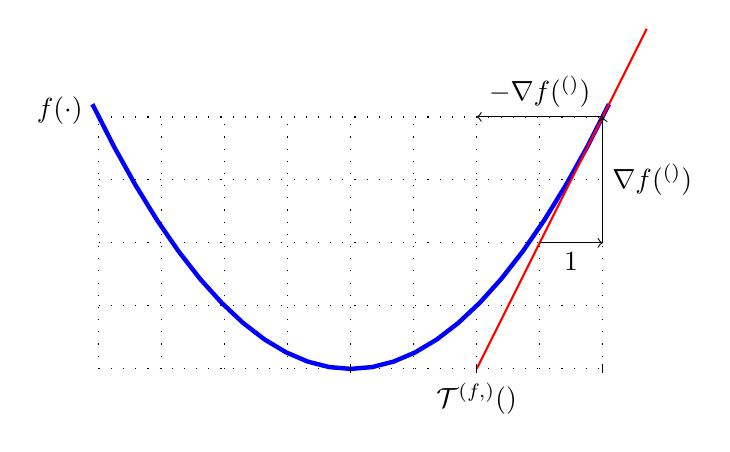
\begin{tikzpicture}[scale=0.8]
					\draw[loosely dotted] (-4,0) grid (4,4);
					\draw[blue, ultra thick, domain=-4.1:4.1] plot (\x,  {(1/4)*\x*\x});
					\draw[red, thick, domain=2:4.7] plot (\x,  {2*\x - 4});
					\draw[<-] (4,4) -- node[right] {$\nabla f(\weights^{(\itercntr)})$} (4,2);
					\draw[->] (4,4) -- node[above] {$-\lrate \nabla f(\weights^{(\itercntr)})$} (2,4);
					\draw[<-] (4,2) -- node[below] {$1$} (3,2) ;
					%\draw[->] (-4.25,0) -- (4.25,0) node[right] {$a$};
					\node[left] at (-4.1, 4.1) {$f(\cdot)$}; 
					\draw[shift={(0,0)}] (0pt,2pt) -- (0pt,-2pt) node[below] {$\overline{\weights}$};
					\draw[shift={(4,0)}] (0pt,2pt) -- (0pt,-2pt) node[below] {$\weights$};
					\draw[shift={(2,0)}] (0pt,2pt) -- (0pt,-2pt) node[below] {$\mathcal{T}^{(f,\lrate)}(\weights)$};
				\end{tikzpicture}
			\end{center}
			\caption{Il passo del\gls{gradient} \eqref{equ_def_gd_basic_dict} mappa un dato vettore $\weights$ 
			nel vettore aggiornato $\weights'$. Esso definisce un operatore 
			$\mathcal{T}^{(f,\lrate)}(\cdot): \mathbb{R}^{\nrfeatures} \rightarrow \mathbb{R}^{\nrfeatures}:
			 \weights \mapsto \widehat{\weights}$.}
			\label{fig_basic_GD_step_single_dict}
		\end{figure}
		Si noti che il passo del \gls{gradient} \eqref{equ_def_gd_basic_dict} ottimizza localmente - 
		in un \gls{neighborhood} la cui dimensione è determinata dalla \gls{stepsize} $\lrate$ - un’approssimazione lineare 
		della \gls{function} $f(\cdot)$. Una \gls{generalization} naturale di \eqref{equ_def_gd_basic_dict} consiste nell’ottimizzare localmente 
		la \gls{function} stessa – invece della sua approssimazione lineare – in modo tale che
		\begin{align} 
		\label{equ_approx_gd_step_dict}
		\widehat{\weights} = \argmin_{\weights' \in \mathbb{R}^{\dimlocalmodel}} f(\weights')\!+\!(1/\lrate)\normgeneric{\weights-\weights'}{2}^2. 
		\end{align}
		Usiamo intenzionalmente lo stesso simbolo $\lrate$ per indicare il \gls{parameter} in \eqref{equ_approx_gd_step_dict} 
		così come fatto per la \gls{stepsize} in \eqref{equ_def_gd_basic_dict}. Più grande sarà il valore di $\lrate$ scelto in 
		\eqref{equ_approx_gd_step_dict}, maggiore sarà il progresso che l'aggiornamento farà rispetto alla riduzione del valore della
		\gls{function} $f(\widehat{\weights})$. Si noti che, analogamente al passo del \gls{gradient} \eqref{equ_def_gd_basic_dict}, 
		anche l'aggiornamento \eqref{equ_approx_gd_step_dict} definisce un operatore 
		parametrizzato dalla \gls{function} $f(\cdot)$ e dal \gls{learnrate} $\lrate$. Per una \gls{function} \gls{convex}
		$f(\cdot)$, tale operatore è noto come \gls{proxop} di $f(\cdot)$ \cite{ProximalMethods}. 
					\\ 
		Si veda anche: \gls{differentiable}, \gls{function}, \gls{gradient}, \gls{stepsize}, \gls{neighborhood}, 
		\gls{generalization}, \gls{parameter}, \gls{learnrate}, \gls{convex}, \gls{proxop}.},
	first={passo del gradiente},
	firstplural={passi del gradiente},
	plural={passi del gradiente},
	text={passo del gradiente}
}
	
\newglossaryentry{contractop}
{name={operatore di contrazione},
	description={Un\index{operatore di contrazione} operatore $\fixedpointop: \mathbb{R}^{\nrfeatures} \rightarrow \mathbb{R}^{\nrfeatures}$
		è una contrazione se, per qualche $\contractfac \in [0,1)$,
		\begin{equation} 
			\nonumber
			\normgeneric{ \fixedpointop \weights\!-\!\fixedpointop \weights'}{2}  \leq  \contractfac	\normgeneric{\weights\!-\!\weights'}{2} \mbox{ holds for any } \weights,\weights' \in \mathbb{R}^{\nrfeatures}.
		\end{equation}
	},
	first={operatore di contrazione},
	text={operatore di contrazione}, 
	firstplural={operatori di contrazione}, 
	plural={operatori di contrazione}
}
	

\newglossaryentry{proxop}
{name={operatore di prossimità},
	description={Data\index{operatore di prossimità} una \gls{function}  
		\gls{convex} $f(\weights')$, definiamo il suo operatore di prossimità come \cite{ProximalMethods}, \cite{Bauschke:2017} 
		$$\proximityop{f(\cdot)}{\weights}{\rho}\defeq \argmin_{\weights' \in \mathbb{R}^{\dimlocalmodel}} \bigg[ f(\weights')\!+\!(\rho/2) \normgeneric{\weights- \weights'}{2}^{2}\bigg] \mbox{ with } \rho > 0. $$ 
		Come illustrato nella Figura \ref{fig_proxoperator_opt_dict}, calcolare l'operatore di prossimità
		consiste nella minimizzazione di una versione penalizzata di $f(\weights')$. La penalizzazione è data dalla  
		distanza euclidea quadratica, opportunamente scalata, rispetto a un vettore fissato $\weights$ (ossia il vettore su cui si applica l'operatore di prossimità). 
		L'operatore di prossimità può essere interpretato come una \gls{generalization} del \gls{gradstep}, definito
		per una \gls{function} $f(\weights')$ \gls{smooth} e \gls{convex}. Infatti, eseguire un 
		\gls{gradstep} con \gls{stepsize} $\lrate$ a partire dal vettore corrente $\weights$ 
		equivale ad applicare l'operatore di prossimità della \gls{function} $\tilde{f}(\weights')= \big( \nabla f(\weights)\big)^{T} (\weights'-\weights)$, 
		con $\rho=1/\lrate$.
			\begin{figure}[H]
			\begin{center}
				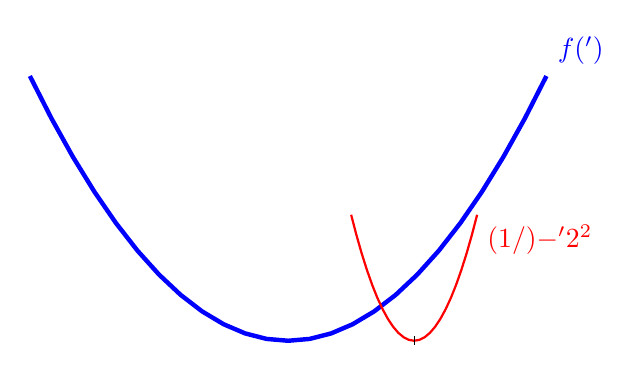
\begin{tikzpicture}[scale=0.8]
					% Original quadratic function
					\draw[blue, ultra thick, domain=-4.1:4.1] plot (\x, {(1/4)*\x*\x}) node[above right] {$f(\weights')$};		
					% Quadratic function with larger curvature, centered at w = 2
					\draw[red, thick, domain=1:3] plot (\x, {2*(\x - 2)*(\x - 2)}) node[below right] {$(1/\lrate)\normgeneric{\weights-\weights'}{2}^{2}$};
					% Axes
					% Minimum point of second curve
					\draw[shift={(2,0)}] (0pt,2pt) -- (0pt,-2pt) node[below] {$\weights$};
					%\node at (2,0.5) [anchor=north] {$\weights$};
				\end{tikzpicture}
			\end{center}
			\caption{Un \gls{gradstep} generalizzato aggiorna un vettore $\weights$ minimizzando una versione 
			penalizzata della \gls{function} $f(\cdot)$. Il termine di penalizzazione è rappresentato dalla distanza 
			euclidea quadratica, opportunamente scalata, tra la variabile di ottimizzazione $\weights'$ e il vettore assegnato $\weights$.	
			\label{fig_proxoperator_opt_dict}}
		\end{figure}
		Si veda anche: \gls{convex}, \gls{function}, \gls{generalization}, \gls{gradstep}, \gls{smooth}, \gls{stepsize}.},
	first={operatore di prossimità},
	text={operatore di prossimità}
}

\newglossaryentry{proximable}
{name={prossimabile},
	description={Una\index{prossimabile} 
		\gls{function} \gls{convex} per cui l'\gls{proxop} può essere calcolato in modo efficiente,è  
		talvolta indicata come prossimabile o semplice \cite{Condat2013}.
					\\ 
		Si veda anche: \gls{convex}, \gls{function}, \gls{proxop}.},
	first={prossimabile},
	text={prossimabile}
}


\newglossaryentry{connected}
{name={grafo connesso}, 
	description={Un\index{grafo connesso} 
		\gls{graph} non orientato $\graph=\pair{\nodes}{\edges}$ è connesso se ogni 
		sottoinsieme non vuoto $\nodes' \subset \nodes$ possiede almeno un arco che lo connette a $\nodes \setminus \nodes'$.
					\\ 
		Si veda anche: \gls{graph}.}, 
	first={grafo connesso},
	text={grafo connesso}
}
	

\newglossaryentry{mvndist}
{name={distribuzione normale multivariata}, 
	description={La\index{distribuzione normale multivariata} distribuzione normale multivariata, 
 		indicata con $\mvnormal{\meanvecgeneric}{\covmtxgeneric}$, è un \gls{probmodel} fondamentale
 		per \glspl{featurevec} numerici di dimensione fissa $\nrfeatures$. 
 		Definisce una famiglia di \glspl{probdist} su \glspl{rv} vettoriali
 		$\featurevec \in \mathbb{R}^{\nrfeatures}$~\cite{BertsekasProb}, \cite{GrayProbBook}, \cite{Lapidoth09}. 
 		Ogni distribuzione appartenente a questa famiglia è determinata univocamente dal vettore della \gls{mean}  
 		$\meanvecgeneric \in \mathbb{R}^{\nrfeatures}$ e dalla \gls{covmtx} $\covmtxgeneric \in \mathbb{R}^{\nrfeatures \times \nrfeatures}$. 
 		Quando la \gls{covmtx} $\covmtxgeneric$ è invertibile, la sua \gls{probdist} è 
 		determinata univocamente dalla seguente \gls{pdf}:
 		\[
 		p(\featurevec) = 
 		\frac{1}{\sqrt{(2\pi)^{\nrfeatures} \determinant{\covmtxgeneric}}} 
 		\exp\left( -\frac{1}{2} 
 		(\featurevec - \meanvecgeneric)^T \covmtxgeneric^{-1} 
 		(\featurevec - \meanvecgeneric) \right).
 		\]
 		Si noti che la \gls{pdf} è definita solo quando $\covmtxgeneric$ è invertibile.
     		Più in generale, ogni \gls{rv} $\featurevec \sim \mvnormal{\meanvecgeneric}{\covmtxgeneric}$ 
     		ammette la seguente rappresentazione:
		\[\featurevec \!=\! \mA \vz \!+\!\meanvecgeneric,
		\]
		dove $\vz \sim \mvnormal{\mathbf{0}}{\mathbf{I}}$ è una \gls{stdnormvec} 
		e $\mA \in \mathbb{R}^{\nrfeatures \times \nrfeatures}$ soddisfa $\mA \mA^T = \covmtxgeneric$. 
		Questa rappresentazione è valida anche quando la \gls{covmtx} $\covmtxgeneric$ è singolare, 
		nel qual caso $\mA$ non è necessariamente a rango completo \cite[Ch. 23]{Lapidoth2017}.\\ 
		La famiglia delle distribuzioni normali multivariate si distingue tra i \glspl{probmodel} relative a quantità numeriche, 
		almeno per i seguenti motivi: in primo luogo, tale famiglia è chiusa rispetto alle trasformazioni affini, ovvero, 
		\[ 
		\featurevec \sim \mathcal{N}(\meanvecgeneric,\covmtxgeneric) \mbox{ implies } 
		\mB\featurevec\!+\!\vc \sim \mathcal{N}\big( \mB\meanvecgeneric+\vc,\mB \covmtxgeneric \mB^{T} \big). 
		\]
		In secondo luogo, la \gls{probdist} $\mathcal{N}(\mathbf{0},\covmtxgeneric)$ massimizza l'\gls{entropy} 
		differenziale tra tutte le distribuzioni che condividono la medesima \gls{covmtx} $\covmtxgeneric$ \cite{coverthomas}. 
		\\ 
		Si veda anche: \gls{probmodel}, \gls{featurevec}, \gls{probdist}, \gls{rv}, \gls{covmtx}, \gls{pdf}, \gls{stdnormvec}, 
		\gls{gaussrv}, \gls{mean}, \gls{entropy}.}, 
	first={distribuzione normale multivariata},
	text={distribuzione normale multivariata}
}

\newglossaryentry{stdnormvec}
{name={vettore normale standard}, 
	description={Un\index{vettore normale standard} vettore normale standard è un vettore aleatorio  $\vx=\big(x_{1},\ldots,x_{\nrfeatures}\big)^{T}$ 
		i cui elementi sono \glspl{gaussrv} \gls{iid} $x_{\featureidx} \sim \mathcal{N}(0,1)$. 
		Si tratta di un caso particolare di una \gls{mvndist}, $\vx \sim \mathcal(\mathbf{0},\mathbf{I})$.
		\\ 
		Si veda anche: \gls{iid}, \gls{gaussrv}, \gls{mvndist}, \gls{rv}.}, 
	first={vettore normale standard},
	text={vettore normale standard}
}

\newglossaryentry{statasp}
{name={aspetti statistici}, 
	description={Con aspetti statistici\index{aspetti statistici} 
		di un metodo di \gls{ml} ci riferiamo alla \glspl{probdist} (e alle sue proprietà) dei risultati che il metodo 
		produce quando i \gls{data} forniti in ingresso seguono un dato \gls{probmodel}.					
		\\ 
		Si veda anche: \gls{ml}, \gls{probdist}, \gls{probmodel}, \gls{data}.},
	first={aspetti statistici},
	text={aspetti statistici}
}

\newglossaryentry{compasp}
{name={aspetti computazionali}, 
	description={Con aspetti computazionali\index{aspetti computazionali} di un metodo di \gls{ml}Ci riferiamo principalmente alle 
	risorse computazionali necessarie per la sua implementazione. Ad esempio, se un metodo di \gls{ml} impiega tecniche di 
	ottimizzazione iterative per risolvere \gls{erm}, i suoi aspetti computazionali comprendono: 1) Quante 
	operazioni aritmetiche sono necessarie per eseguire una singola iterazione (ossia un \gls{gradstep}); 
		and 2) Quante iterazioni sono richieste per ottenere \gls{modelparams} utili. Un esempio 
		significativo di tecnica di ottimizzazione iterativa è il \gls{gd}.
					\\ 
		Si veda anche: \gls{ml}, \gls{erm}, \gls{gradstep}, \gls{modelparams}, \gls{gd}.}, 
	first={aspetti computazionali},
	text={aspetti computazionali}
}

\newglossaryentry{zerooneloss}{name={perdita $\bf 0/1$},
	description={La \gls{loss} $0/1$\index{perdita $0/1$} $\lossfunczo{\pair{\featurevec}{\truelabel}}{\hypothesis}$ 
		misura la qualità di un \gls{classifier} $\hypothesis(\featurevec)$ che fornisce una 
		\gls{prediction} $\predictedlabel$ (ad esempio, applicando una soglia come in \eqref{equ_def_threshold_bin_classifier_dict}) 
		per l'\gls{label} $\truelabel$ di un \gls{datapoint} con \glspl{feature} $\featurevec$. Essa vale $0$ se 
		la \gls{prediction} è corretta, ovvero, 
		$\lossfunczo{\pair{\featurevec}{\truelabel}}{\hypothesis}=0$ quando $\predictedlabel=\truelabel$. Vale $1$ se la
		 \gls{prediction} è sbagliata, ovvero, $\lossfunczo{\pair{\featurevec}{\truelabel}}{\hypothesis}=1$ 
		quando $\predictedlabel\neq\truelabel$.
				\\ 
		Si veda anche: \gls{loss}, \gls{classifier}, \gls{prediction}, \gls{label}, \gls{datapoint}, \gls{feature}.},
	sort=zerooneloss, 
    	first={perdita $0/1$},
	text={perdita $0/1$}
}

\newglossaryentry{probability}
{name={probabilità}, 
	description={Assegniamo\index{probabilità} un valore di probabilità, tipicamente scelto 
	nell’intervallo $[0,1]$, a ciascun evento che può verificarsi in un esperimento casuale 
		\cite{BillingsleyProbMeasure}, \cite{BertsekasProb}, \cite{HalmosMeasure},  \cite{KallenbergBook}.},
	first={probabilità},
	firstplural={probabilità},
	plural={probabilità},
	text={probabilità}
}
	
\newglossaryentry{underfitting}
{name={underfitting},
	description={Si consideri\index{underfitting} 
		un metodo di \gls{ml} che utilizza \gls{erm} per apprendere un'\gls{hypothesis} con il \gls{minimum} \gls{emprisk} 
		su un dato \gls{trainset}. Un tale metodo sta effettuando un underfitting del \gls{trainset} se non è in grado di 
		apprendere un’\gls{hypothesis} con un \gls{emprisk} sufficientemente basso sul \gls{trainset}. 
		Se un metodo è in underfitting, tipicamente non riuscirà nemmeno ad apprendere un'\gls{hypothesis} con 
		un \gls{risk} contenuto.
					\\ 
		Si veda anche: \gls{ml}, \gls{erm}, \gls{hypothesis}, \gls{minimum}, \gls{emprisk}, \gls{trainset}, \gls{risk}.},
	first={underfitting},
	text={underfitting}
}

\newglossaryentry{overfitting}
{name={overfitting},
	description={Si consideri\index{overfitting}  
		un metodo di \gls{ml} che utilizza \gls{erm} per apprendere un'\gls{hypothesis} con il \gls{minimum} \gls{emprisk} 
		su un dato \gls{trainset}. Un tale metodo sta effettuando un overfitting del \gls{trainset} se apprende 
		un'\gls{hypothesis} con un basso \gls{emprisk} sul \gls{trainset}, ma con una \gls{loss} significativamente più elevata 
		al di fuori del \gls{trainset}.
					\\ 
		Si veda anche: \gls{generalization}, \gls{erm},  \gls{validation}, \gls{gengap}.},
	first={overfitting},
	text={overfitting}
}

\newglossaryentry{gdpr}
{name={general data protection regulation (GDPR)},
	description={Il\index{general data protection regulation (GDPR)} GDPR (Regolamento generale sulla protezione dei dati)
			è stato emanato dall’Unione Europea (UE), ed è entrato in vigore il 25 maggio 2018 \cite{GDPR2016}. 
			Esso tutela la riservatezza e i diritti relativi ai \gls{data} delle persone fisiche nell’UE. Il GDPR influisce in 
			modo significativo sulle modalità di raccolta, conservazione e utilizzo dei \gls{data} nelle applicazioni di \gls{ml}.  
			Le disposizioni principali includono::
			\begin{itemize}
				\item \Gls{dataminprinc}: i sistemi di \gls{ml} devono impiegare esclusivamente la quantità minima necessaria di \gls{data} personali 
				per il perseguimento delle loro finalità. 
				\item \Gls{transparency} and \gls{explainability}: i sistemi di \gls{ml} devono consentire agli utenti 
				di comprendere in che modo vengono prese le decisioni che li riguardano.				
				\item Diritti degli interessati: gli utenti devono avere la possibilità di accedere, 
				rettificare e cancellare i propri \gls{data}, nonché di opporsi al processo decisionale automatizzato e alla profilazione.
				\item Responsabilizzazione: le organizzazioni devono garantire adeguate misure di sicurezza dei \gls{data} 
				e dimostrare la conformità al GDPR mediante documentazione e audit periodici.
			\end{itemize}
		Si veda anche: \gls{data}, \gls{ml}, \gls{dataminprinc}, \gls{transparency}, \gls{explainability}.}, 
	first={general data protection regulation (GDPR)},
	text={GDPR}
}
	
\newglossaryentry{gaussrv}{name={variabile aleatoria Gaussiana},description={
		Una \index{variabile aleatoria Gaussiana} \gls{rv} Gaussiana standard è una 
		\gls{rv} a valori reali $x$ con \gls{pdf} \cite{BertsekasProb}, \cite{GrayProbBook}, \cite{papoulis}
		\begin{equation}
			\nonumber
			p(x) = \frac{1}{\sqrt{2\pi}} \exp^{-x^2/2}. 
		\end{equation}
		Data una \gls{rv} Gaussiana standard $x$, è possibile costruire una generica \gls{rv} Gaussiana $x'$ con 
		\gls{mean} $\mu$ e \gls{variance} $\sigma^2$ tramite $x' \defeq \sigma (x+\mu)$. La \gls{probdist} di una 
		\gls{rv} Gaussiana è detta distribuzione normale, indicata con $\mathcal{N}(\mu,\sigma)$.  
		\\ 
		Un vettore aleatorio Gaussiano $\featurevec \in \mathbb{R}^{\featuredim}$ con 
		\gls{covmtx} $\mathbf{C}$ e \gls{mean} ${\bm \mu}$ può essere costruito come \cite{GrayProbBook}, \cite{papoulis}, \cite{Lapidoth09}
		\[
		\featurevec \defeq \mathbf{A} \vz + {\bm \mu},
		\]
		dove $\vz \defeq \big( z_{1}, \ldots, z_{\featuredim} \big)^{T}$ è un 
		vettore di \glspl{rv} gaussiane standard \gls{iid}, e $\mA \in \mathbb{R}^{\featuredim \times \featuredim}$ è una matrice qualsiasi 
		tale che $\mA \mA^{T} = \mC$.
		La \gls{probdist} di un vettore aleatorio gaussiano è detta \gls{mvndist}, ed è indicata con $\mathcal{N}({\bm \mu}, \mathbf{C})$.
		\\
		I vettori casuali gaussiani si ottengono come marginali a dimensione finita di \glspl{GaussProc}, i quali definiscono distribuzioni 
		congiunte gaussiane consistenti su insiemi di indici arbitrari (potenzialmente infiniti) \cite{Rasmussen2006Gaussian}. 
		\\
		Le \glspl{rv} Gaussiane sono ampiamente utilizzate come \glspl{probmodel} nell'analisi statistica dei metodi di \gls{ml}. La loro 
		rilevanza deriva in parte dal \gls{clt}, che rappresenta una formulazione matematica rigorosa della seguente regola empirica: la 
		media di un grande numero di \glspl{rv} indipendenti (non necessariamente Gaussiane) tende a una \gls{rv} Gaussiana
		\cite{ross2013first}.
		\\
		Rispetto ad altre \glspl{probdist}, la \gls{mvndist} si distingue anche per il fatto che— in un senso matematicamente preciso—
		rappresenta l'\gls{uncertainty} massima. Tra tutti i vettori aleatori continui con una data matrice di covarianza $\mC$, il vettore 
		aleatorio Gaussiano $\vx \sim \mathcal{N}({\bm \mu}, \mathbf{C})$ massimizza l’\gls{entropy} differenziale \cite[Th. 8.6.5]{coverthomas}. 
		Questo rende i \glspl{GaussProc} una scelta naturale per catturare l’\gls{uncertainty} (o la mancanza di conoscenza) 
		in assenza di ulteriori informazioni strutturali.
		\\
		Si veda anche: \gls{mvndist}, \gls{GaussProc}, \gls{probmodel}, \gls{clt}, \gls{entropy}.
		},
		first={variabile aleatoria Gaussiana},
		text={variabile aleatoria Gaussiana}
}
		
\newglossaryentry{clt}
{name={teorema del limite centrale (TLC)},
	description={Si consideri una successione di \glspl{rv} \gls{iid} \( \feature^{(\sampleidx)} \), per \( \sampleidx = 1, 2, \ldots \), 
		ciascuna avente \gls{mean} nulla e \gls{variance} finita \( \sigma^2 > 0 \). 
		Il \index{teorema del limite centrale (TLC)} TLC stabilisce che la somma normalizzata 
		\[
		s^{(\samplesize)} \defeq \frac{1}{\sqrt{\samplesize}} \sum_{\sampleidx = 1}^{\samplesize} \feature^{(\sampleidx)} 
		\]
		converge in distribuzione, per \( \samplesize \to \infty \), ad una \gls{gaussrv} con \gls{mean} nulla 
		e \gls{variance} \( \sigma^2 \) \cite[Proposition~2.17]{AsympVanderVaartBook}.
		Un modo elegante per dimostrare il TLC si basa sull’analisi della \gls{characteristicfunc} della somma normalizzata \( s^{(\samplesize)} \). 
		Sia $ \phi(t) = \expect \big\{ \exp \big( j t \feature \big) \big\}$ (con l'unità immaginaria $j = \sqrt{-1}$) 
		la \gls{characteristicfunc} comune ad ogni addendo $\feature^{(\sampleidx)}$, e sia \( \phi^{(\samplesize)}(t) \) 
		la \gls{characteristicfunc} di \( s^{(\samplesize)} \). Si definisca un operatore \( \mathcal{T} \) operante sulle \glspl{characteristicfunc} 
		tale che
		\[
		\phi^{(\samplesize)}(t) = \mathcal{T}(\phi^{(\samplesize-1)})(t) \defeq \phi\left( \frac{t}{\sqrt{\samplesize}} \right) \cdot \phi^{(\samplesize-1)}\left( \frac{\sqrt{\samplesize-1}}{\sqrt{\samplesize}} t \right).
		\]
		Questa \gls{fixedpointiter} descrive l’effetto prodotto dall’aggiunta ricorsiva di una \gls{rv} \gls{iid} $\featurevec^{(\samplesize)}$ 
		seguita dal relativo ridimensionamento. Applicando ripetutamente l’operatore \( \mathcal{T} \), la funzione\( \phi^{(\samplesize)}(t) \) 
		converge al corrispondente punto fisso
		\[
		\phi^*(t) = e^{-t^2 \sigma^2 / 2},
		\]
		che rappresenta la \gls{characteristicfunc} di una \gls{gaussrv} con \gls{mean} nulla e \gls{variance} 
		\( \sigma^2 \). Le generalizzazioni del TLC ammettono \glspl{rv} dipendenti o non identicamente distribuite \cite[Section~2.8]{AsympVanderVaartBook}.
\begin{figure}
	\centering
	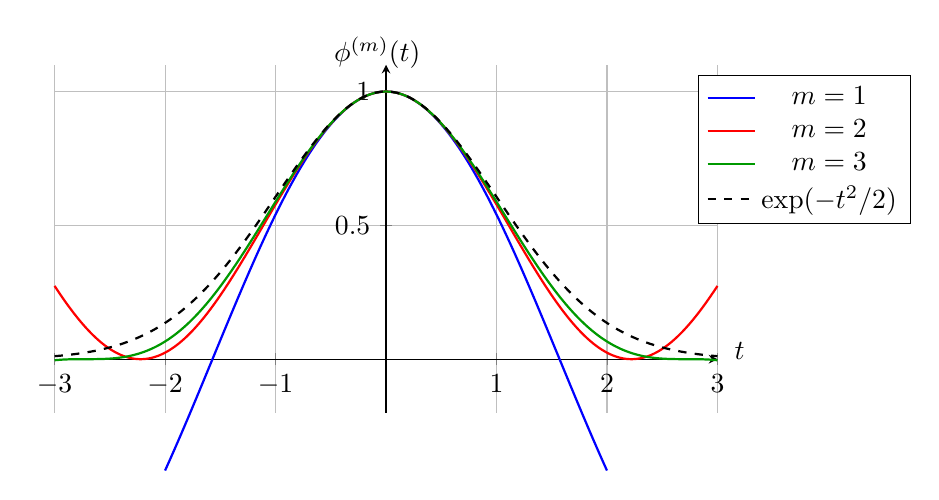
\begin{tikzpicture}
		\begin{axis}[
			width=10cm,
			height=6cm,
			xlabel={},
			ylabel={},
			legend style={at={(0.97,0.97)}, anchor=north west},
			domain=-3:3,
			ylabel style={
				yshift=10pt   % shift label up by 10pt
			},
			samples=400,
			ymin=-0.2, ymax=1.1,
			axis lines=middle,
			  clip=false,
			grid=both,
			]
		\addplot[thick, blue,domain=-2:2] {cos(x/sqrt(1) r)^1};
		\addlegendentry{$m=1$}
		\addplot[thick, red] {cos(x/sqrt(2) r)^2};
		\addlegendentry{$m=2$}
		\addplot[thick, green!60!black] {cos(x/sqrt(3) r)^3};
		\addlegendentry{$m=3$}
		\addplot[thick, dashed, black] {exp(-x^2/2)};
		\addlegendentry{$\exp(-t^2/2)$}
		\node[anchor=south, rotate=0] at (axis cs:-0.08,1.05) {$\phi^{(m)}(t)$};
		\node[anchor=north, rotate=0] at (axis cs: 3.2,0.1) {$t$};
		\end{axis}
	\end{tikzpicture}
	\caption{\Glspl{characteristicfunc} di somme normalizzate di \glspl{rv} \gls{iid} $x^{(\sampleidx)} \in \{-1,1\}$ 
		per $\sampleidx=1,\ldots,\samplesize$ comparate al limite Gaussiano.}
\end{figure}
		\\ 
		Si veda anche: \gls{rv}, \gls{gaussrv}.},
	first={teorema del limite centrale (TLC)},
	text={TLC}
}



\newglossaryentry{GaussProc}
{name={Processo Gaussiano (GP)},plural={GP},
  description={Un \index{Processo Gaussiano (GP)}GP è una collezione di \glspl{rv} 
  	$\{f(\featurevec)\}_{\featurevec \in \featurespace}$ in cui ciascuna \gls{rv} è indicizzata 
	da un vettore $\featurevec$ proveniente da un qualche spazio di input $\featurespace$, 
	tale che, per ogni sottoinsieme finito 
  	$\featurevec^{(1)}, \ldots, \featurevec^{(\samplesize)} \in \featurespace$, 
  	le corrispondenti \glspl{rv} $f(\featurevec^{(1)}, \ldots, \featurevec^{(\samplesize)}$ abbiano una 
	distribuzione gaussiana multivariata congiunta:
  	\[
  	\left( f(\featurevec^{(1)}, \ldots, \featurevec^{(\samplesize)} \right) \sim \mathcal{N}(\boldsymbol{\mu}, \mathbf{K}).
  	\]
  	Per uno spazio di input $\featurespace$ fissato, un GP è 
	completamente specificato (o parametrizzato) da 
  	\begin{itemize}
  		\item una \gls{function} di \gls{mean} $\mu(\featurevec) = \expect\{ f(\featurevec)\}$
  		\item e una \gls{function} di covarianza $\kernelmap{\featurevec}{\featurevec'}= \expect\{ \big(f(\featurevec)-\mu(\featurevec)\big) \big(f(\featurevec')-\mu(\featurevec')\big) \big\}$.
  	\end{itemize}
  	\text{Esempio:} Possiamo interpretare la distribuzione delle temperature in Finlandia (in uno specifico 
	istante nel tempo) come la \gls{realization} di un GP $f(\featurevec)$, dove ogni vettore di input 
	$\featurevec = (\text{lat}, \text{lon})$ 
  	rappresenta una posizione geografica. Le osservazioni di temperatura provenienti dalle stazioni 
	meteorologiche del \gls{fmi} forniscono 
  	\glspl{sample} di $f(\featurevec)$ in posizioni specifiche (si veda la Figura \ref{fig_gp_FMI_dict}). Un GP ci 
	consente di prevedere la temperatura nelle vicinanze delle stazioni del \gls{fmi} e di quantificare 
	l'\gls{uncertainty} di tali previsioni. 
  	\begin{figure}[H]
  	\begin{center}
  \begin{tikzpicture}
\begin{axis}[
	axis equal,
	hide axis,
	scale=1.2,
	xmin=17, xmax=32,
	ymin=55, ymax=71,
%	width=15cm,
%	height=20cm,
	clip=true
	]
	% --- Finland border (polyline) ---
	\addplot[
	color=black,
	thick
	] table [x=lon, y=lat, col sep=comma] {assets/finland_border.csv};
	% --- FMI sample stations ---
	\addplot[
	only marks,
	mark=*,
	mark options={fill=blue},
	color=black
	] table [x=lon, y=lat, col sep=comma] {assets/fmi_stations_subset.csv};
	% Draw manual axes
	\draw[->, thick] (axis cs:19,59) -- (axis cs:25.5,59) node[anchor=west] {lon};
	\draw[->, thick] (axis cs:19,59) -- (axis cs:19,65.5) node[anchor=south] {lat};
\end{axis}
\end{tikzpicture}
\vspace*{-15mm}
\end{center}
\caption{Possiamo interpretare la distribuzione della temperatura sul territorio finlandese come una 
	\gls{realization} di un GP indicizzato dalle coordinate geografiche e campionato presso le stazioni 
	meteorologiche \gls{fmi} (indicate dai punti blu). \label{fig_gp_FMI_dict}}
\end{figure}
Si veda anche: \gls{rv}, \gls{mean}, \gls{function}, \gls{realization}, \gls{fmi}, \gls{sample}, \gls{uncertainty}.}, 
first = {GP}, 
text = {GP}
}


\newglossaryentry{trustAI}
{name={intelligenza artificiale affidabile (IA affidabile)},
	description={Oltre all'\gls{compasp} e all'\gls{statasp}, un terzo aspetto progettuale fondamentale dei 
	metodi di \gls{ml} è la loro affidabilità\index{intelligenza artificiale affidabile (IA affidabile)} \cite{pfau2024engineeringtrustworthyaideveloper}. 
		L’Unione Europea ha individuato sette requisiti chiave  per un'
		\gls{ai} affidabile (che si basano tipicamente su metodi \gls{ml}) \cite{ALTAIEU}: 
	\begin{enumerate}[label=\arabic*)]
		\item Intervento e sorveglianza umani;
		\item \Gls{robustness} tecnica e sicurezza;
		\item Privacy e governance dei \gls{data};
		\item \Gls{transparency};
		\item Diversità, non discriminazione ed equità;
		\item Benessere sociale e ambientale;
		\item Accountability. 
	\end{enumerate}
		Si veda anche: \gls{compasp}, \gls{statasp}, \gls{ml}, \gls{ai}, \gls{robustness}, \gls{data}, \gls{transparency}.},
	first={intelligenza artificiale affidabile (IA affidabile)},
	text={IA affidabile}
}

\newglossaryentry{sqerrloss}
{name={funzione di perdita quadratica},
	description={La funzione di \gls{loss} quadratica \index{funzione di perdita quadratica}
	Quantifica l’errore di \gls{prediction} di una 
		\gls{hypothesis} $\hypothesis$ nel predire un'\gls{label} numerica $\truelabel \in \mathbb{R}$ 
		a partire dalle \glspl{feature} $\featurevec$ di un \gls{datapoint}. È definito come 
		\begin{equation} 
			\nonumber
			\lossfunc{(\featurevec,\truelabel)}{\hypothesis} \defeq \big(\truelabel - \underbrace{\hypothesis(\featurevec)}_{=\predictedlabel} \big)^{2}. 
		\end{equation} 
			\\ 
		Si veda anche: \gls{loss}, \gls{prediction}, \gls{hypothesis}, \gls{label}, \gls{feature}, \gls{datapoint}.},
	first={funzione di perdita quadratica},
	text={funzione di perdita quadratica}
}


 \newglossaryentry{projection}
 {name={proiezione}, 
       description={Si consideri\index{proiezione} un sottoinsieme  $\paramspace \subseteq \mathbb{R}^{\dimlocalmodel}$ dello \gls{euclidspace} $\dimlocalmodel$-dimensionale. Definiamo la proiezione  $\projection{\paramspace}{\weights}$
	   di un vettore $\weights \in \mathbb{R}^{\dimlocalmodel}$ su $\paramspace$ come
	   \begin{equation} 
   	   	\label{equ_def_proj_generic_dict}
  	    	\projection{\paramspace}{\weights} = \aargmin_{\weights' \in \paramspace} \normgeneric{\weights - \weights'}{2}. 
        	    \end{equation}
	    In altre parole, $\projection{\paramspace}{\weights}$ è il vettore in $\paramspace$ 
	    più vicino a $\weights$. La proiezione è ben definita solo per quei sottoinsiemi $\paramspace$ 
	    per i quali esiste il suddetto \gls{minimum} \cite{BoydConvexBook}.
		 			\\ 
	    Si veda anche: \gls{euclidspace}, \gls{minimum}.},
	first={proiezione},
	text={proiezione}
}


\newglossaryentry{projgd}
{name={projected gradient descent (projected GD)},
description={Consider an \gls{erm}-based method that uses a parametrized \gls{model} with  
\gls{paramspace} $\paramspace \subseteq \mathbb{R}^{\dimlocalmodel}$. Even if 
the \gls{objfunc} of \gls{erm} is \gls{smooth}, we cannot use basic \gls{gd}, as 
it does not take into account contraints on the optimization variable (i.e., the \gls{modelparams}). 
Projected\index{projected gradient descent (projected GD)} \gls{gd} 
extends basic \gls{gd} to handle constraints on the optimization variable (i.e., the \gls{modelparams}). 
A single iteration of projected \gls{gd} consists of first taking a \gls{gradstep} 
and then projecting the result back onto the \gls{paramspace}.
\begin{figure}[H]
	\begin{center}
		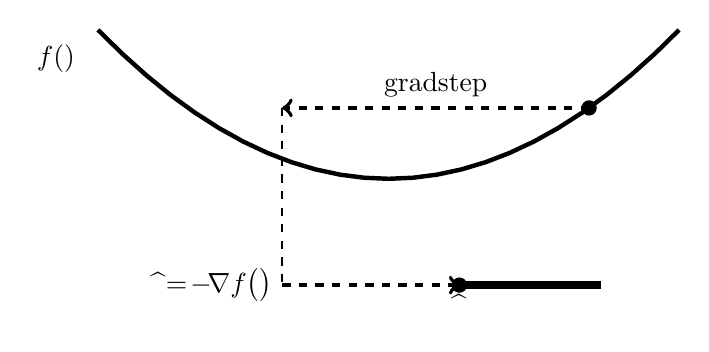
\begin{tikzpicture}[scale=0.9]
			\node [right] at (-5.1,1.7) {$f(\weights)$} ;
			\draw[ultra thick, domain=-4.1:4.1] plot (\x,  {(1/8)*\x*\x});
		%	\draw[dashed, thick, domain=1:3.6] plot (\x,  {\x - 1}) node[right] {$ f\big(\weights^{(\itercntr)}\big)\!+\!\big(\weights\!-\!\weights^{(\itercntr)}\big)^{T} \nabla f\big(\weights^{(\itercntr)}\big)$};
			\draw [fill] (2.83,1) circle [radius=0.1] node[right] {$\weights$};
			\draw[line width =0.5mm,dashed,->] (2.83,1) -- node[midway,above] {\gls{gradstep}} (-1.5,1);
			\draw[line width =0.2mm,dashed] (-1.5,1) --(-1.5,-1.5)  node [below, left]{$\widehat{\weights}=\weights\!-\!\lrate \nabla f\big(\weights\big)$} ;
			\draw[line width =0.5mm,dashed,->] (-1.5,-1.5)  -- node[midway,above] {} (1,-1.5) ; 
			\draw [fill] (1,-1.5) circle [radius=0.1] node[below] {$\projection{\paramspace}{\widehat{\weights}}$};
			\draw[line width=1mm] (1,-1.5) -- (3,-1.5) node[midway, above] {$\paramspace$};
		\end{tikzpicture}
		\vspace*{-5mm}
	\end{center}
	\caption{Projected \gls{gd} augments a basic \gls{gradstep} with a \gls{projection} back 
	onto the constraint set $\paramspace$.}
	\label{fig_projected_GD_dict}
\end{figure}
		See also: \gls{erm}, \gls{model}, \gls{paramspace}, \gls{objfunc}, \gls{smooth}, \gls{gd}, \gls{modelparams}, \gls{gradstep}, \gls{projection}.},
	first={projected gradient descent (projected GD)},
	text={projected GD}
}


\newglossaryentry{diffpriv}
{name={differential privacy (DP)},
  description={Consider\index{differential privacy (DP)} some \gls{ml} method $\algomap$ 
  	that reads in a \gls{dataset} (e.g., the \gls{trainset} 
  	used for \gls{erm}) and delivers some output $\algomap(\dataset)$. The output 
  	could be either the learned \gls{modelparams} or the \glspl{prediction} for specific \glspl{datapoint}. 
  	DP is a precise measure of \gls{privleakage} incurred by revealing the 
  	output. Roughly speaking, an \gls{ml} method is differentially private if the \gls{probdist} 
  	of the output $\algomap(\dataset)$ remains largely unchanged if the \gls{sensattr} 
  	of one \gls{datapoint} in the \gls{trainset} is changed. Note that DP 
  	builds on a \gls{probmodel} for an \gls{ml} method, i.e., we interpret its output $\algomap(\dataset)$ 
  	as the \gls{realization} of an \gls{rv}. The randomness in the output can be ensured 
  	by intentionally adding the \gls{realization} of an auxiliary \gls{rv} (i.e., adding noise) to 
  	the output of the \gls{ml} method.
				\\ 
	See also: \gls{privleakage}, \gls{sensattr}, \gls{privattack}, \gls{privfunnel}.}, 
  first={DP}, 
  text={DP} 
}

\newglossaryentry{robustness}
{name={robustezza},
	description={La robustezza\index{robustezza} è un requisito fondamentale per l'\gls{trustAI}. Essa si 
	riferisce alla proprietà di un sistema di \gls{ml} di mantenere prestazioni accettabili anche quando 
	sottoposto a diverse forme di perturbazioni. Tali perturbazioni possono riguardare le \glspl{feature} 
		di un singolo \gls{datapoint}, con l’obiettivo di manipolare la \gls{prediction} fornita da un \gls{model}
		di \gls{ml} addestrato. 
		La robustezza comprende inoltre la \gls{stability} dei metodi basati su \gls{erm} nei confronti delle 
		perturbazioni del \gls{trainset}. Tali perturbazioni possono manifestarsi nell’ambito di attacchi di 
		\gls{datapoisoning}.
		\\ 
		Si veda anche: \gls{trustAI}, \gls{ml}, \gls{feature}, \gls{datapoint}, \gls{prediction}, \gls{model}, \gls{stability}, \gls{erm}, \gls{trainset}, \gls{datapoisoning}, \gls{attack}.}, 
	first={robustezza}, 
	text={robustezza} 
}

\newglossaryentry{stability}
{name={stabilità},
	description={La stabilità\index{stabilità} è una proprietà desiderabile di un metodo di \gls{ml} $\algomap$ 
	che mappa un 
		\gls{dataset} $\dataset$ (ad esempio, un \gls{trainset}) in un output $\algomap(\dataset)$. L'output
		$\algomap(\dataset)$ può corrispondere ai \gls{modelparams} appresi o alla \gls{prediction} fornita 
		dal \gls{model} addestrato per uno specifico \gls{datapoint}. Intuitivamente, $\algomap$ è stabile se 
		piccole variazioni nel \gls{dataset} di input $\dataset$ comportano piccole variazioni nell’output 
		$\algomap(\dataset)$. Esistono diverse nozioni formali di stabilità che consentono di ottenere dei 
		vincoli sull’errore di \gls{generalization} o sul \gls{risk} del metodo (see \cite[Ch.~13]{ShalevMLBook}).
		Per favorire una comprensione intuitiva, si considerino i tre \glspl{dataset} rappresentati in Fig. 
		\ref{fig_three_data_stability_dict}, each 
		ciascuno dei quali è ugualmente probabile secondo la medesima \gls{probdist} generatrice dei 
		\gls{data}. Poiché i \gls{modelparams} ottimali sono determinati da tale \gls{probdist} sottostante, un 
		metodo di \gls{ml} accurato $\algomap$ dovrebbe restituire lo stesso output (od uno molto simile) 
		$\algomap(\dataset)$ 
		per tutti e tre i \glspl{dataset}. In altre parole, ogni $\algomap$ utile deve essere robusto rispetto alla 
		variabilità nelle \glspl{realization} dei \glspl{sample} provenienti dalla medesima \gls{probdist}, ossia 
		deve essere stabile.		
		\begin{figure}[H]
			\centering
			\begin{tikzpicture}
				\begin{axis}[
				%title={Stem Plots of 3 Datasets},
				    axis lines=none,
					xlabel={$\sampleidx$},
					ylabel={},
					legend pos=north west,
					ymin=0, ymax=10,
					xtick={1,2,3,4,5},
				%	ymajorgrids=true,
					grid style=dashed,
					every axis plot/.append style={very thick}
					]
					% Dataset 1
					\addplot+[only marks,mark=*] coordinates {
						(1,2) (2,4) (3,3) (4,5) (5,7)
					};
				%	\addlegendentry{$\dataset^{(*)}$}
					% Dataset 2
					\addplot+[only marks,mark=square*] coordinates {
						(1,3) (2,2) (3,6) (4,4) (5,5)
					};
				%	\addlegendentry{$\dataset^{(\square)}$}
					% Dataset 3
					\addplot+[only marks,mark=triangle*] coordinates {
						(1,5) (2,7) (3,4) (4,6) (5,3)
					};
				%	\addlegendentry{$\dataset^{(\triangle)}$}
				\end{axis}
			\end{tikzpicture}
			\caption{Tre \glspl{dataset} $\dataset^{(*)}$, $\dataset^{(\square)}$, and $\dataset^{(\triangle)}$, 
				ognuno campionato indipendentemente dalla stessa \gls{probdist}. Un metodo di \gls{ml} 
				stabile dovrebbe restituire output simili qualora fosse addestrato su uno qualsiasi di questi 
				\glspl{dataset}. \label{fig_three_data_stability_dict}}
		\end{figure}
		Si veda anche: \gls{ml}, \gls{dataset}, \gls{trainset}, \gls{modelparams}, \gls{prediction}, \gls{model}, \gls{datapoint}, \gls{generalization}, \gls{risk}, \gls{data}, \gls{probdist}, \gls{sample}, \gls{realization}.}, 
	first={stabilità}, 
	text={stabilità} 
}


\newglossaryentry{privprot}
{name={protezione della privacy},
     description={Si consideri\index{protezione della privacy} un metodo di \gls{ml} $\algomap$ che prende in 
     input un \gls{dataset} $\dataset$ e restituisce un output $\algomap(\dataset)$. Esso può corrispondere ai 
	 	\gls{modelparams} appresi $\widehat{\weights}$ oppure alla \gls{prediction} 
	 	$\learnthypothesis(\featurevec)$ ottenuta per uno specifico \gls{datapoint} con \glspl{feature} 
	 	$\featurevec$. Molte applicazioni di rilievo in \gls{ml} riguardano \glspl{datapoint} 
		che rappresentano individui. Ogni \ \gls{datapoint} è caratterizzato da \glspl{feature} $\featurevec$, 
		da un’eventuale \gls{label} $\truelabel$, e da un \gls{sensattr} $\sensattr$ (ad esempio, una diagnosi 
		medica recente). 
		In termini generali, la protezione della privacy implica che non sia possibile dedurre, dall’output 
		$\algomap(\dataset)$, 
		alcuno degli \glspl{sensattr} dei \glspl{datapoint} nel $\dataset$. Matematicamente, la protezione 
		della privacy richiede la non invertibilità della \gls{map} $\algomap(\dataset)$. Tuttavia, in generale il 
		solo fatto di rendere $\algomap(\dataset)$ non invertibile risulta spesso insufficiente per garantire la 
		protezione della privacy: è infatti necessario che $\algomap(\dataset)$ sia sufficientemente non 
		invertibile. 
					\\ 
		Si veda anche: \gls{ml}, \gls{dataset}, \gls{modelparams}, \gls{prediction}, \gls{datapoint}, \gls{feature}, \gls{label}, \gls{sensattr}, \gls{map}.}, 
	first={protezione della privacy}, 
	text={protezione della privacy} 
}


\newglossaryentry{privleakage}
{name={fuga di dati sensibili},
	description={Consider\index{privacy leakage} un’applicazione di \gls{ml} che elabora un 
		\gls{dataset} $\dataset$ e fornisce un qualche output, come le \glspl{prediction} 
		ottenute per nuovi \glspl{datapoint}. La fuga di dati sensibili si verifica se l’output 
		veicola dati su una \gls{feature} privata (o sensibile) di un \gls{datapoint} 
		(che potrebbe essere un individuo) del $\dataset$. Basandosi su un \gls{probmodel} 
		per la generazione dei \gls{data}, è possibile quantificare la fuga di dati mediante la 
		\gls{mutualinformation} 
		tra l’output e la \gls{feature} sensibile. Un’altra misura quantitativa è la \gls{diffpriv}. Le relazioni tra le 
		diverse misure sono state analizzate in letteratura (see \cite{InfThDiffPriv}). 
				\\ 
		Si veda anche: \gls{mutualinformation}, \gls{diffpriv}, \gls{privattack}, \gls{gdpr}. }, 
	first={fuga di dati sensibili}, 
	text={fuga di dati sensibili} 
}



\newglossaryentry{probmodel}
{
	name={modello probabilistico}, plural={modelli probabilistici},
	description={Un \gls{model} probabilistico\index{probabilistic model} interpreta i \glspl{datapoint} 
		come \glspl{realization} di \glspl{rv} con una \gls{probdist} congiunta. Tale \gls{probdist} congiunta coinvolge 
		tipicamente dei \glspl{parameter}che devono essere scelti manualmente oppure appresi mediante
metodi di inferenza statistica, come la stima di \gls{maxlikelihood} \cite{LC}.					
									\\ 
		Si veda anche: \gls{model}, \gls{datapoint}, \gls{realization}, \gls{rv}, \gls{probdist}, \gls{parameter}, \gls{maxlikelihood}. }, 
	first = {modello probabilistico}, text={modello probabilistico} 
}



\newglossaryentry{mean}
{name={media}, plural={medie},
	description={La \index{media} media di una \gls{rv} $\featurevec$, a 
 		valori in uno \gls{euclidspace} $\mathbb{R}^{\dimlocalmodel}$, è il suo 
 		\gls{expectation} $\expect\{\featurevec\}$. Essa è definita come l'integrale di Lebesgue  
 		di $\featurevec$ rispetto alla \gls{probdist} $P$ sottostante (si veda, ad esempio, 
		\cite{RudinBookPrinciplesMatheAnalysis} o \cite{BillingsleyProbMeasure}), ovvero,
		\[
			\expect\{\featurevec\} = \int_{\mathbb{R}^{\dimlocalmodel}} \featurevec \, \mathrm{d}P(\featurevec).
		\] 
		Talvolta è utile considerare la media come la soluzione del seguente problema 
		di minimizzazione del \gls{risk} \cite{BertsekasProb}:
		\[
			\expect\{\featurevec\} = \argmin_{\vc \in \mathbb{R}^{\nrfeatures}} 
			\expect \big\{\normgeneric{\featurevec - \vc}{2}^{2}\big \}.
		\] 
		Usiamo inoltre il termine per riferirci alla media di una sequenza finita
		$\vx^{(1)}, \ldots, \vx^{(\samplesize)} \in \mathbb{R}^{\dimlocalmodel}$. Tuttavia, 
		queste due definizioni sono sostanzialmente equivalenti. Infatti, è possibile utilizzare la sequenza
		$\vx^{(1)}, \ldots, \vx^{(\samplesize)} \in \mathbb{R}^{\dimlocalmodel}$ per costruire una
		\gls{rv} discreta $\widetilde{\vx}=\vx^{(I)}$, dove l'indice $I$ è scelto in modo uniforme 
		a caso dall'insieme $\{1,\ldots,\samplesize\}$. La media di $\widetilde{\vx}$ coincide  
		esattamente con la media $\frac{1}{\samplesize} \sum_{\sampleidx=1}^{\samplesize} \vx^{(\sampleidx)}$.
				\\ 
		Si veda anche: \gls{rv}, \gls{expectation}, \gls{probdist}.}, 
	first={media},
	text={media} 
}


\newglossaryentry{median}
{name={mediana}, 
 plural={mediane},
 description={Una\index{mediana} mediana $\med(x)$ di una \gls{rv} a valori reali $x$ 
 è un qualunque numero $m \in \mathbb{R}$ tale che $\prob{ x \leq m} \geq 1/2$ e $\prob{ x \geq m} \geq 1/2$ \cite{LC}. 
 \begin{figure}
	\begin{center}
	\begin{tikzpicture}
  \begin{axis}[
    axis lines=middle,
    xlabel={$m$},
    ylabel={},
    ymin=0, ymax=1.1,
    xmin=-2, xmax=6,
    xtick=\empty,
    ytick={0,1/2,1},
    domain=-2:6,
    samples=200,
    width=10cm,
    height=6cm,
    smooth,
    enlargelimits=true,
    clip=false
  ]
    % Shifted sigmoid CDF
	\addplot[thick, blue, name path=cdf] {1/(1 + exp(-(x - 1)))} node[pos=0.5, above, yshift=15pt] {$\prob{x \leq m}$};    % Vertical and horizontal ruler at F(x) = 0.5
    \draw[dashed, gray] (axis cs:1,0) -- (axis cs:1,0.5); % vertical
    \draw[dashed, gray] (axis cs:-2,0.5) -- (axis cs:1,0.5); % horizontal
    % Mark the median point
    \filldraw[red] (axis cs:1,0.5) circle (2pt);
  %  \node[below left] at (axis cs:1,0.5) {\footnotesize $(x{=}1,\ F(x){=}\tfrac{1}{2})$};
    % Label next to curve
  \end{axis}
\end{tikzpicture} 
\end{center}
 \end{figure}  
 Possiamo definire la mediana $\med(\dataset)$ 
 di un\gls{dataset} $\dataset = \{ x^{(1)}, \ldots, x^{(\samplesize)} \in \mathbb{R} \}$ 
 attraverso una specifica \gls{rv} $\tilde{x}$ naturalmente associata al $\dataset$. 
 In particolare, questa \gls{rv} è costruita come $\tilde{x} = x^{(I)}$, dove l'indice $I$ 
 è scelto in modo uniforme a caso dall’insieme $\{1,\ldots,\samplesize\}$, ossia $\prob{I = \sampleidx}=1/\samplesize$ per 
 ogni $\sampleidx=1,\ldots,\samplesize$. Se la \gls{rv} $x$ è integrabile, una mediana di $x$ 
 è la soluzione del seguente problema di ottimizzazione:
  $$\min_{x' \in \mathbb{R}} \expect{|x - x'|}.$$ 
 Analogamente alla \gls{mean}, anche la mediana di un \gls{dataset} $\dataset$ può essere utilizzata
 per stimare i \glspl{parameter} di un \gls{probmodel} sottostante. Rispetto 
 alla \gls{mean}, la mediana è meno influenzata dagli \glspl{outlier}. Ad esempio, 
 la median di un \gls{dataset} $\dataset$ con più di un \gls{datapoint} non varia 
 anche se si aumenta arbitrariamente il valore del massimo elemento del $\dataset$. Al contrario, 
 la \gls{mean} aumenterà anch’essa arbitrariamente.
 	\begin{figure}
		\centering
		\begin{tikzpicture}[scale=0.7, y=0.5cm, x=0.5cm]
			\begin{scope}
				\foreach \x/\y in {
					1/2, 4/3, 7/4
				} {
					\draw[dashed, gray] (\x, 0) -- (\x, \y);
					\filldraw[blue] (\x, \y) circle (2pt);
					\node[circle, inner sep=0pt] (ptA\x) at (\x, \y) {};
				}
				\draw[dashed, thick, darkgreen] (0.5, 3) -- (10.5, 3) node[right] {$\med(\dataset)$};
				\node at (5.5, -4) {(a) \Gls{dataset} originale $\dataset$.};
			\end{scope}
			\begin{scope}[xshift=12cm]
				\foreach \x/\y in {
					1/2, 4/3, 7/10
				} {
					\draw[dashed, gray] (\x, 0) -- (\x, \y);
					\filldraw[blue] (\x, \y) circle (2pt);
					\node[circle, inner sep=0pt] (ptB\x) at (\x, \y) {};
				}
				\draw[dashed, thick, darkgreen] (0.5, 3) -- (10.5, 3) node[right] {$\med\big(\widetilde{\dataset}\big)$};
				\node[above right=2pt and 2pt, red] at (ptB7) {outlier};
				\node at (5.5, -4) {(b) \Gls{dataset} rumoroso $\widetilde{\dataset}$ in cui è presente un \gls{outlier}.};
			\end{scope}
		\end{tikzpicture}
		\caption{La median è resistente alla presenza di \gls{outlier}.}
	\end{figure}
	\\ 
		Si veda anche: \gls{mean}, \gls{robustness}, \gls{outlier}.}, 
	first = {mediana}, 
	text={mediana} 
}



\newglossaryentry{variance}
{
	name={varianza},
	description={La\index{varianza} varianza di una \gls{rv} a valori reali $\feature$ è definita come il \gls{expectation} 
		$\expect\big\{ \big( x - \expect\{x \} \big)^{2} \big\}$ del quadrato della differenza tra $\feature$ 
		ed il suo \gls{expectation} $\expect\{x \}$. Estendiamo questa definizione alle \glspl{rv} vettoriali $\featurevec$ 
		come $\expect\big\{ \big\| \featurevec - \expect\{\featurevec \} \big\|_{2}^{2} \big\}$.
					\\ 
		Si veda anche: \gls{rv}, \gls{expectation}.} ,
	first={varianza},
	text={varianza} 
}

\newglossaryentry{nn}
{name={nearest neighbor (NN)},
	description={I metodi di Nearest Neighbor (ossia "ricerca del vicino più prossimo")\index{nearest neighbor (NN)} apprendono una \gls{hypothesis} 
		$\hypothesis: \featurespace \rightarrow \labelspace$ il cui valore di \gls{function} $\hypothesis(\featurevec)$ 
		è determinato unicamente dai Nearest Neighbors (vicini più prossimi) all’interno di uno specifico \gls{dataset}. Metodi differenti impiegano \glspl{metric} diverse per individuare i Nearest Neighbors. Se i \glspl{datapoint} 
		sono caratterizzati da \glspl{featurevec} numerici, possiamo utilizzare come \gls{metric} le loro distanze euclidee.
					\\ 
		Si veda anche: \gls{hypothesis}, \gls{function}, \gls{dataset}, \gls{metric}, \gls{datapoint}, \gls{featurevec}, \gls{neighbors}.},
	first={nearest neighbor (NN)},
	text={NN} 
}

\newglossaryentry{neighborhood}
{name={vicinato},
	description={Il\index{vicinato} vicinato di un nodo $\nodeidx \in \nodes$ è 
		il sottoinsieme dei nodi costituito dai \gls{neighbors} di $\nodeidx$.
				\\ 
		Si veda anche: \gls{neighbors}.},
	first={vicinato},
	text={vicinato} 
}

\newglossaryentry{neighbors}
{name={vicini},
	description={I\index{vicini} vicini di un nodo $\nodeidx \in \nodes$ 
		all'interno di un \gls{empgraph} sono quei nodi $\nodeidx' \in \nodes \setminus \{ \nodeidx\}$ 
		che sono connessi (tramite un arco) al nodo $\nodeidx$.
				\\ 
		Si veda anche: \gls{empgraph}.},
	first={vicini},
	text={vicini} 
}

\newglossaryentry{bias}
{name={bias},
	description={Si consideri\index{bias} un metodo di \gls{ml} che utilizza uno \gls{hypospace} parametrizzato $\hypospace$. 
		Esso apprende i \gls{modelparams} $\weights \in \mathbb{R}^{\dimlocalmodel}$ impiegando il \gls{dataset} $$\dataset=\big\{ \pair{\featurevec^{(\sampleidx)}}{\truelabel^{(\sampleidx)}} \big\}_{\sampleidx=1}^{\samplesize}.$$ 
		Per studiarne le proprietà, interpretiamo tipicamente i \glspl{datapoint} come \glspl{realization} 
		di \glspl{rv} \gls{iid}, ossia $$\truelabel^{(\sampleidx)} = \hypothesis^{(\overline{\weights})}\big( \featurevec^{(\sampleidx)} \big) + \bm{\varepsilon}^{(\sampleidx)}, \sampleidx=1, \ldots, \samplesize.$$ 
		Possiamo allora vedere il metodo di \gls{ml} come un estimatore $\widehat{\weights}$ 
		calcolato a partire da $\dataset$ (ad esempio risolvendo \gls{erm}). Il bias (al quadrato) della stima $\widehat{\weights}$ 
		si definisce quindi come $\biasterm^{2} \defeq \big\| \expect \{ \widehat{\weights}  \}- \overline{\weights}\big\|_{2}^{2}$.
					\\ 
		Si veda anche: \gls{ml}, \gls{hypospace}, \gls{modelparams}, \gls{dataset}, \gls{datapoint}, \gls{realization}, \gls{iid}, \gls{rv}, \gls{erm}.},
	first={bias},
	text={bias} 
}

\newglossaryentry{classification}
{name={classificazione},
	description={La classificazione\index{classificazione} consiste nell’assegnare un'\gls{label} 
	a valori discreti $\truelabel$ ad un dato \gls{datapoint}, basandosi esclusivamente sulle sue 
 		\glspl{feature} $\featurevec$. L'\gls{label} $\truelabel$ appartiene a un insieme finito,
		come ad esempio $\truelabel \in \{-1,1\}$ o $\truelabel \in \{1, \ldots, 19\}$, e rappresenta la categoria 
		cui il corrispondente \gls{datapoint} appartiene.
						\\ 
		Si veda anche: \gls{label}, \gls{datapoint}, \gls{feature}.},
	first={classificazione},
	text={classificazione} 
}


\newglossaryentry{privfunnel}
{name={privacy funnel},
	description={Il\index{privacy funnel} privacy funnel ("imbuto della privacy") è un metodo per apprendere \glspl{feature} 
		rispettose della privacy dei \glspl{datapoint} \cite{PrivacyFunnel}.
				\\ 
		Si veda anche: \gls{feature}, \gls{datapoint}.},
 	first={privacy funnel},
	text={privacy funnel} 
}



\newglossaryentry{condnr}
{name={numero di condizionamento},
	description={Il numero di condizionamento\index{numero di condizionamento} $\kappa(\mathbf{Q}) \geq 1$ di una 
	matrice definita positiva $\mathbf{Q} \in \mathbb{R}^{\featurelen \times \featurelen}$ è il rapporto 
		$\alpha /\beta  $ tra l'\gls{eigenvalue} massimo $\alpha$ e l'\gls{eigenvalue} minimo $\beta$ di 
		$\mathbf{Q}$. Il numero di condizionamento risulta utile per l’analisi dei metodi \gls{ml}. 
		La complessità computazionale dei \gls{gdmethods} per la \gls{linreg} dipende in modo cruciale dal numero di 	
		condizionamento della matrice $\mQ = \mX \mX^{T}$, dove $\mX$ è la \gls{featuremtx} 
		del \gls{trainset}. Pertanto, da un punto di vista computazionale, è preferibile adottare \glspl{feature} dei 
		\glspl{datapoint} tali che $\mQ$ presenti un numero di condizionamento prossimo a $1$.
					\\ 
		Si veda anche: \gls{eigenvalue}, \gls{ml}, \gls{gdmethods}, \gls{linreg}, \gls{featuremtx}, \gls{trainset}, \gls{feature}, \gls{datapoint}.},
	first={numero di condizionamento},
	text={numero di condizionamento} 
}

\newglossaryentry{classifier}
{name={classificatore},
	description={Un classificatore\index{classificatore} è una \gls{hypothesis} (ovvero, una \gls{map}) $\hypothesis(\featurevec)$ 
		utilizzata per prevedere un'\gls{label} che assume valori in uno \gls{labelspace} finito. Potremmo usare 
		direttamente il valore della \gls{function} $\hypothesis(\featurevec)$ come \gls{prediction} $\predictedlabel$ per 
		l'\gls{label}. Tuttavia, è consuetudine impiegare una \gls{map} $\hypothesis(\cdot)$ che fornisca una quantità 
		numerica. La \gls{prediction} si ottiene quindi mediante l’applicazione di una soglia decisionale (tresholding). 
		Ad esempio, in un problema di \gls{classification} binaria con uno \gls{labelspace} $\labelspace \in  \{ -1,1\}$, 
		si può utilizzare una \gls{map} \gls{hypothesis} reale $\hypothesis(\featurevec) \in \mathbb{R}$ 
		come classificatore. La \gls{prediction} $\predictedlabel$ si ottiene quindi applicando una soglia decisionale,  
		 \begin{equation} 
		 	\label{equ_def_threshold_bin_classifier_dict}
		 	\predictedlabel =1   \mbox{ for } \hypothesis(\featurevec)\!\geq\!0 \mbox{ and } 	\predictedlabel =-1  \mbox{ otherwise.}
	 		\end{equation}
 		Un classificatore può essere descritto tramite le sue \glspl{decisionregion} $\decreg{a}$, corrispondenti a ciascun 
		possibile valore di \gls{label} $a \in \labelspace$.
					\\ 
		Si veda anche: \gls{hypothesis}, \gls{map}, \gls{label}, \gls{labelspace}, \gls{function}, \gls{prediction}, \gls{classification}, \gls{decisionregion}. },
	first={classificatore},
	text={classificatore} 
}


\newglossaryentry{emprisk}
{name={rischio empirico},
  description={Il \gls{risk} empirico\index{rischio empirico} $\emprisk{\hypothesis}{\dataset}$ 
  	di un'\gls{hypothesis} su un \gls{dataset} $\dataset$ è la media della \gls{loss} sostenuta 
	da $\hypothesis$ quando viene applicata ai \glspl{datapoint} in $\dataset$.
				\\ 
		Si veda anche: \gls{risk}, \gls{hypothesis}, \gls{dataset}, \gls{loss}, \gls{datapoint}.},
  first={rischio empirico},
  text={rischio empirico} 
}

\newglossaryentry{nodedegree}
{name={grado nodale},
	description={Il grado\index{grado nodale} $\nodedegree{\nodeidx}$ di un nodo $\nodeidx \in \nodes$ 
		in un \gls{graph} non orientato è il numero dei suoi \gls{neighbors}, ovvero $\nodedegree{\nodeidx} \defeq \big|\neighbourhood{\nodeidx}\big|$.
					\\ 
		Si veda anche: \gls{graph}, \gls{neighbors}.},
	first={grado nodale},
	text={grado nodale} 
}

\newglossaryentry{graph}
{name={grafo},
	description={Un grafo\index{grafo} $\graph = \pair{\nodes}{\edges}$ è una struttura costituita da  
	un insieme di nodi $\nodes$ e da un insieme di archi $\edges$. Nella sua formulazione più generale, 
	un grafo è descritto da una \gls{map} che associa a ciascun arco $\edgeidx \in \edges$ una coppia di nodi 
	\cite{RockNetworks}. 
		Una famiglia rilevante di grafi è quella dei grafi semplici non orientati. Un grafo semplice 
		non orientato si ottiene identificando ciascun arco $\edgeidx \in \edges$ con due nodi distinti $\{\nodeidx,\nodeidx'\}$. 
		Weighted graphs also specify numeric \gls{weights} $\edgeweight_{\edgeidx}$ for each 
		edge $\edgeidx \in \edges$.
					\\ 
		Si veda anche: \gls{map}, \gls{weights}.},
	first={grafo},
	text={grafo} 
}

\newglossaryentry{uncertainty}
{name={incertezza},
	description={Nel contesto del \gls{ml},con il termine incertezza\index{incertezza} ci si riferisce alla presenza di 
	molteplici esiti plausibili o di diverse \glspl{explanation} basate sui \gls{data} a disposizione. Ad esempio, la
		\gls{prediction} $\hat{\hypothesis}(\featurevec)$ generata da un \gls{model} di \gls{ml} 
		$\hat{\hypothesis}$ addestrato riflette spesso un intervallo di valori possibili per la vera \gls{label} 
		di uno specifico \gls{datapoint}. 
	 	Quanto più è ampio tale intervallo, tanto maggiore risulta l’incertezza associata. La teoria della \gls{probability} 
	 	ci permette di rappresentare, quantificare e ragionare sull’incertezza in modo matematicamente rigoroso.					\\ 
		Si veda anche: \gls{probmodel}, \gls{risk}, \gls{entropy}, \gls{variance}. },
	first={incertezza},
	text={incertezza}
}

\newglossaryentry{ucb}
{name={upper confidence bound (UCB)},
	description={Si consideri\index{upper confidence bound (UCB)} un'applicazione di \gls{ml} 
		che richiede di selezionare, in ogni istante temporale $\iteridx$, un'azione $\action_{\iteridx}$ 
		da un insieme finito di alternative  $\actionset$. L’utilità derivante dalla selezione dell’azione $\action_{\iteridx}$ 
		è quantificata da un segnale numerico di \gls{reward} $\reward^{(\action_{\iteridx})}$. 
		Un \gls{probmodel} ampiamente utilizzato per questo tipo di problema  
		è l'impostazione del \gls{mab} \gls{stochastic} \cite{Bubeck2012}. In questo \gls{model}, 
		la \gls{reward} $\reward^{(\action)}$ è considerata come la \gls{realization} di una \gls{rv} 
		con \gls{mean} ignota $\mu^{(\action)}$. Idealmente, sceglieremmo sempre l’azione con il più 
		alto valore atteso per la \gls{reward} $\mu^{(\action)}$, ma tali 
		\glspl{mean} sono sconosciute e devono essere stimate dai \gls{data} osservati. Il semplice 
		fatto di scegliere l’azione con la stima più elevata  $\widehat{\mu}^{(\action)}$ può condurre a esiti subottimali a 
		causa dell’\gls{uncertainty}. La strategia Upper Confidence Bound ("limite superiore di confidenza")
		affronta tale questione selezionando le azioni non solo in base alle stime delle loro \glspl{mean}, ma 
		anche integrando un termine che riflette l'\gls{uncertainty} di queste stime — privilegiando pertanto le azioni 
		caratterizzate sia da una potenziale elevata \gls{reward} sia da una significativa \gls{uncertainty}. 
		In \cite{Bubeck2012} sono stabilite garanzie teoriche per le prestazioni delle strategie UCB, 
		tra cui limiti logaritmici sul \gls{regret}..
					\\ 
		Si veda anche: \gls{ml}, \gls{reward}, \gls{probmodel}, \gls{stochastic}, \gls{mab}, \gls{model}, \gls{realization}, \gls{rv}, \gls{mean}, \gls{data}, \gls{uncertainty}, \gls{regret}.},
	first={upper confidence bound (UCB)},
	text={UCB} 
}

\newglossaryentry{mab}
{name={multi-armed bandit (MAB)},
	description={Un problema MAB\index{multi-armed bandit (MAB)}(Bandito Multibraccia) descrive uno scenario di decisioni 
	ripetute in cui, a ogni istante $\iteridx$, un agente deve selezionare una fra le azioni disponibili (denominate “braccia”) 
	appartenenti a un insieme finito $\actionset$. 
	Ogni braccio $\action\in\actionset$ fornisce una \gls{stochastic} \gls{reward} $\reward^{(\action)}$, 
	estratta da una \gls{probdist} ignota con \gls{mean} $\mu^{(\action)}$.
		L'obiettivo dell'agente è massimizzare nel tempo la \gls{reward} cumulativa, bilanciando strategicamente 
		l’esplorazione (ovvero la raccolta di informazioni sui bracci incerti) e l’utilizzo (ovvero la selezione dei bracci noti 
		per le loro buone prestazioni).Questo equilibrio è quantificato dalla nozione di \gls{regret}, che misura il divario di 
		prestazioni tra la strategia dell’apprendente e la strategia ottimale che seleziona sempre il miglior braccio.
		I problemi MAB costituiscono un \gls{model} fondamentale nell'\gls{onlinelearning}, nel reinforcement learning e 
		nella progettazione sperimentale sequenziale \cite{Bubeck2012}.
					\\ 
		Si veda anche: \gls{stochastic}, \gls{reward}, \gls{probdist}, \gls{mean}, \gls{regret}, \gls{model}.},
	first={MAB},
	text={MAB}
}



\newglossaryentry{optimism in the face of uncertainty}
{name={ottimismo di fronte all’incertezza},
	description={\I metodi di \gls{ml}\index{optimism in the face of uncertainty} apprendono i  \gls{modelparams} $\weights$ 
		in base a un criterio di prestazione $\bar{f}(\weights)$. Tuttavia, di norma non possono accedere 
		direttamente a $\bar{f}(\weights)$, ma si basano su una stima (o approssimazione) $f(\weights)$ di $\bar{f}(\weights)$. 
		A titolo esemplificativo, i metodi basati su \gls{erm} utilizzano la \gls{loss} media su uno specifico 
		\gls{dataset} (vale a dire, il \gls{trainset}) come stima del \gls{risk} di una \gls{hypothesis}.		
		Utilizzando un \gls{probmodel}, è possibile costruire un intervallo di confidenza
		$\big[ l^{(\weights)},  u^{(\weights)} \big]$ per ogni scelta $\weights$ dei \gls{modelparams}. 
		Una costruzione semplice è $l^{(\weights)} \defeq f(\weights) - \sigma/2$, $u^{(\weights)} \defeq f(\weights)+ \sigma/2$, 
	    	with $\sigma$ being a measure of the (expected) deviation of $f(\weights)$ from $\bar{f}(\weights)$.
		Si possono formulare altre costruzioni per quest'intervallo, purché garantiscano che 
		$\bar{f}(\weights) \in\big[ l^{(\weights)},  u^{(\weights)} \big]$ 
		con una \gls{probability} sufficientemente elevata. Un ottimista seleziona i \gls{modelparams} in base al valore
		 $\tilde{f}(\weights) \defeq  l^{(\weights)}$ più favorevole, ma ancora plausibile,
		del criterio di performance. Due esempi di metodi \gls{ml} che utilizzano una tale costruzione ottimistica 
		di una \gls{objfunc} sono \gls{srm} \cite[Ch. 11]{ShalevMLBook} e i metodi di \gls{ucb}  
		per i processi decisionali sequenziali \cite[Sec. 2.2]{Bubeck2012}. 
		\begin{figure}[H]
				\begin{center}
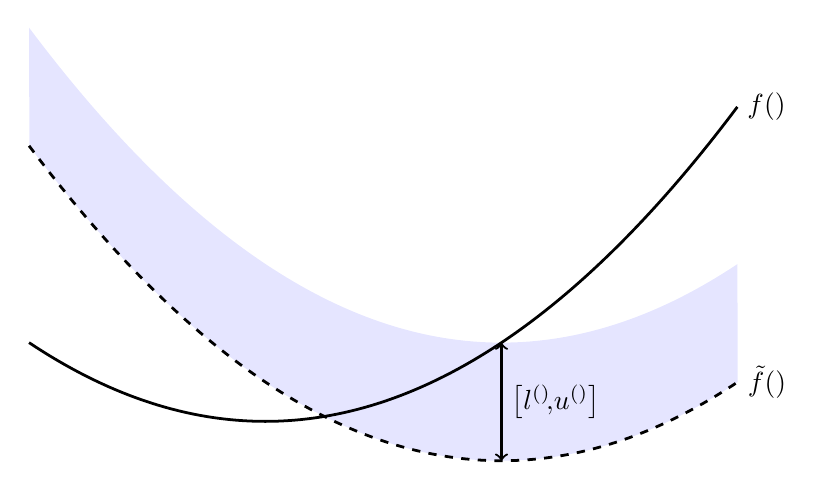
\begin{tikzpicture}[x=3cm, y=1cm]
  % Filled band around the quadratic curve with different boundary curves
\fill[blue!10] 
(-1, 5) -- plot[domain=-2:1, samples=100] ({\x+1}, {\x*\x + 1}) -- 
plot[domain=1:-2, samples=100] ({\x+1}, {\x*\x - 0.5}) -- cycle;
  \node[anchor=west] at (2, 4) {$f(\weights)$};
  \draw[line width=1, domain=-2:1, samples=100,dashed] plot  ({\x+1}, {\x*\x -0.5}) node[right] {$\tilde{f}(\weights)$};
   \draw[line width=1, domain=-1:2, samples=100] plot ({\x}, {\x*\x});
  \draw[<->, thick] (1, -0.5) -- (1, 1) node[midway, right] {$\big[ l^{(\weights)}\!,\!u^{(\weights)} \big]$};
\end{tikzpicture}
\caption{I metodi di \gls{ml} apprendono \gls{modelparams} $\weights$ mediante una stima di $f(\weights)$  
	rispetto al criterio di prestazione ultimo $\bar{f}(\weights)$. Usando un \gls{probmodel}, è possibile utilizzare $f(\weights)$  
	per costruire intervalli di confidenza  $\big[ l^{(\weights)},  u^{(\weights)} \big]$ che contengano $\bar{f}(\weights)$  
	con elevata probabilità. La miglior misura di prestazione plausibile per unascelta specifica $\weights$ di \gls{modelparams} 
	è definita da $\tilde{f}(\weights) \defeq l^{(\weights)}$.} 
	\end{center}
		\end{figure}
		Si veda anche: \gls{ml}, \gls{modelparams}, \gls{erm}, \gls{loss}, \gls{dataset}, \gls{trainset}, \gls{risk}, \gls{hypothesis}, \gls{probmodel}, \gls{probability}, \gls{objfunc}, \gls{srm}, \gls{ucb}.},
	first={ottimismo di fronte all’incertezza},
	text={ottimismo di fronte all’incertezza} 
}
\newglossaryentry{empgraph}
{name={federated learning network (FL network)},
	description={A federated network\index{federated learning network (FL network)} is an undirected weighted \gls{graph} whose 
		nodes represent \gls{data} generators that aim to train a local (or personalized) \gls{model}. 
		Each node in a federated network represents some \gls{device} capable of collecting a \gls{localdataset} 
		and, in turn, train a \gls{localmodel}. 
	    \Gls{fl} methods learn a local \gls{hypothesis} $\localhypothesis{\nodeidx}$, for 
	    each node $\nodeidx \in \nodes$, such that it incurs small \gls{loss} on the \gls{localdataset}s.},first={federated learning network (FL network)},text={FL network} 
}

\newglossaryentry{norm}
{name={norma},
	description={A norm\index{norm} è una funzione che associa a ciascun elemento (vettore) 
	di uno spazio vettoriale lineare un numero reale non negativo. Tale funzione deve essere omogenea e definita, e deve soddisfare la disuguaglianza triangolare \cite{HornMatAnalysis}. },
	first={norma},text={norma} 
}

\newglossaryentry{explanation}
{name={explanation},
	description={One approach to make \gls{ml} methods transparent is to provide an 
		explanation\index{explanation} along with the \gls{prediction} delivered by an 
		\gls{ml} method. Explanations can take on many different forms. An explanation 
		could be some natural text or some quantitative measure for the importance 
		of individual \gls{feature}s of a \gls{datapoint} \cite{Molnar2019}. We can also 
		use visual forms of explanations, such as intensity plots for image \gls{classification} \cite{GradCamPaper}.},
	first={explanation},text={explanation} 
}

\newglossaryentry{risk}
{name={risk},
	description={Consider\index{risk} a \gls{hypothesis} $\hypothesis$ used to predict the \gls{label} 
		$\truelabel$ of a \gls{datapoint} based on its \gls{feature}s $\featurevec$. We measure 
		the quality of a particular \gls{prediction} using a \gls{lossfunc} $\lossfunc{(\featurevec,\truelabel)}{\hypothesis}$. 
		If we interpret \gls{datapoint}s as the \gls{realization}s of \gls{iid} \gls{rv}s, 
		also the $\lossfunc{(\featurevec,\truelabel)}{\hypothesis}$ becomes the \gls{realization} 
		of an \gls{rv}. The \gls{iidasspt} allows us to define the risk of a \gls{hypothesis} 
		as the expected \gls{loss} $\expect \big\{\lossfunc{(\featurevec,\truelabel)}{\hypothesis} \big\}$. 
		Note that the risk of $\hypothesis$ depends on both the specific choice for the \gls{lossfunc} and the 
		\gls{probdist} of the \gls{datapoint}s.},
	first={risk},text={risk} 
}

\newglossaryentry{actfun}
{name={activation function},
	description={Each\index{activation function} artificial neuron within an \gls{ann} is 
		assigned an activation function $\actfun(\cdot)$ that maps a weighted combination of 
		the neuron inputs $\feature_{1},\ldots,\feature_{\nrfeatures}$ to a single output 
		value $a = \actfun\big(\weight_{1} \feature_{1}+\ldots+\weight_{\nrfeatures} \feature_{\nrfeatures} \big)$. 
		Note that each neuron is parametrized by the \gls{weights} $\weight_{1},\ldots,\weight_{\nrfeatures}$.},
first={activation function},text={activation function} 
}

\newglossaryentry{distributedalgorithm}
{name={distributed algorithm},
	description={A\index{distributed algorithm} distributed \gls{algorithm} is an \gls{algorithm} designed for 
		a special type of computer: a collection of interconnected computing devices (or nodes). 
		These devices communicate and coordinate their local computations by exchanging 
		messages over a network \cite{IntroDistAlg,ParallelDistrBook}. Unlike a classical \gls{algorithm}, 
		which is implemented on a single \gls{device}, a distributed \gls{algorithm} is 
		executed concurrently on multiple \gls{device}s with computational capabilities. 
		Similar to a classical \gls{algorithm}, a distributed \gls{algorithm} can be modeled as a 
		set of potential executions. However, each execution in the distributed setting involves 
		both local computations and message-passing events. A generic execution might look as 
		follows:
		\[
		\begin{array}{l}
			\text{Node 1: } {\rm input}_1, s_1^{(1)}, s_2^{(1)}, \ldots, s_{T_1}^{(1)}, {\rm output}_1; \\
			\text{Node 2: } {\rm input}_2, s_1^{(2)}, s_2^{(2)}, \ldots, s_{T_2}^{(2)}, {\rm output}_2; \\
			\quad \vdots \\
			\text{Node N: } {\rm input}_N, s_1^{(N)}, s_2^{(N)}, \ldots, s_{T_N}^{(N)}, {\rm output}_N.
		\end{array}
		\]
		Each \gls{device} $\nodeidx$ starts from its own local input and performs a sequence of 
		intermediate computations $s_{\iteridx}^{(\nodeidx)}$ at discrete time instants $\iteridx = 1, \dots, T_\nodeidx$. 
		These computations may depend on both: the previous local computations at the \gls{device} 
		and messages received from other \gls{device}s. One important application of distributed 
		\gls{algorithm}s is in \gls{fl} where a network of \gls{device}s collaboratively train a personal \gls{model} 
		for each \gls{device}. 
		},
	first={distributed algorithm}, text={distributed algorithm}
}


\newglossaryentry{algorithm}
{name={algorithm},
  description={An\index{algorithm} algorithm is a precise, step-by-step specification for 
  	how to produce an output from a given input within a finite number of computational steps \cite{Cormen:2022aa}. 
    For example, an algorithm for training a \gls{linmodel} explicitly describes how to 
	transform a given \gls{trainset} into \gls{modelparams} through a sequence of \gls{gradstep}s. 
    This informal characterization can be formalized rigorously via different mathematical \gls{model}s \cite{Sipser2013}. 
    One very simple \gls{model} of an algorithm is a collection of possible executions. Each execution is a sequence:
    $${\rm input},s_1,s_2,\ldots,s_T,{\rm output}$$ 
    that respects the constraints inherent to the computer executing the algorithm.
	Algorithms may be deterministic, where each input results uniquely in a single execution,
	or randomized, where executions can vary probabilistically. Randomized algorithms 
	can thus be analyzed by modeling execution sequences as outcomes of random experiments, 
	viewing the algorithm as a stochastic process \cite{RandomizedAlgos,BertsekasProb,Gallager13}.
	Crucially, an algorithm encompasses more than just a mapping from input to output; it also includes 
	the intermediate computational steps $s_1,\ldots,s_T$. 
	%. In \textbf{online algorithms}, these intermediate computational steps  can dynamically incorporate additional input data as the execution progresses.
	},
	first={algorithm},text={algorithm} 
}

\newglossaryentry{onlinealgorithm}
{name={online algorithm},
	description={An\index{online algorithm} online \gls{algorithm} processes input \gls{data} incrementally, 
		receiving \gls{data} items sequentially and making decisions or producing outputs (or decisions) immediately 
		without having access to the entire input in advance \cite{HazanOCO,PredictionLearningGames}. 
		Unlike an offline \gls{algorithm}, which has the entire input available from the start, an online \gls{algorithm} 
		must handle uncertainty about future inputs and cannot revise past decisions. Similar to an 
		offline \gls{algorithm}, an online \gls{algorithm} can be modeled formally as a collection of possible 
		executions. However, the execution sequence for an online \gls{algorithm} has a distinct structure:
		$${\rm init},s_1,{\rm out}_{1},{\rm in}_{2},s_2,{\rm out}_{2},\ldots,{\rm in}_{T},s_T,{\rm out}_{T}.$$ 
		Each execution begins from an initial state (\(\text{init}\)) and proceeds through alternating computational steps, 
		outputs (or decisions), and inputs. Specifically, at step \(\iteridx\), the \gls{algorithm} performs a computational step 
		\(s_{\iteridx}\), generates an output \(\text{out}_{\iteridx}\), and then subsequently 
		receives the next input \(\text{in}_{\iteridx+1}\). A notable example of an online \gls{algorithm} in \gls{ml} is 
		\gls{onlineGD} (online gradient descent), which incrementally updates \gls{modelparams} as new \gls{datapoint}s 
		arrive.
	},
	first={online algorithm},text={online algorithm} 
}



%\newglossaryentry{transparency}
%{name={transparency},
%	description={Transparency\index{transparency} is a key requirement for 
%		trustworthy \gls{ai} \cite{HLEGTrustworhtyAI}. In the context of ML methods, 
%		such as \gls{erm}-based methods, transparency is mainly used synonymously 
%		for \gls{explainability} \cite{gallese2023ai,JunXML2020}. However, in the wide 
%		context of \gls{ai} systems, transparency also includes providing information 
%		about limitations and reliability of the \gls{ai} system. As a point in case, \gls{logreg} provides a 
%		quantitative measure of the reliability of a \gls{classification} in the form of the value $|\hypothesis(\featurevec)|$. 
%		Transparency also includes the user interface, by requiring to clearly indicate when a user is 
%		interaction with an \gls{ai} system. Another component of transparency is the documentation 
%		of the system’s purpose, design choices, and intended use cases \cite{Shahriari2017,DatasheetData2021,10.1145/3287560.3287596}. },
%	first={transparency},text={transparency} 
%}

\newglossaryentry{transparency}
{name={transparency},
	description={Transparency\index{transparency} is a fundamental requirement for 
		\gls{trustAI} \cite{HLEGTrustworhtyAI}. In the context of \gls{ml} 
		methods, transparency is often used interchangeably with \gls{explainability} 
		\cite{gallese2023ai,JunXML2020}. However, in the broader scope of \gls{ai} 
		systems, transparency extends beyond \gls{explainability} and includes providing information 
		about the system’s limitations, reliability, and intended use. 
		In medical diagnosis systems, transparency requires disclosing the confidence level 
		for the \gls{prediction}s delivered by a trained \gls{model}. In credit scoring, 
		\gls{ai}-based lending decisions should be accompanied by explanations of 
		contributing factors, such as income level or credit history. These explanations 
		allow humans (e.g., a loan applicant) to understand and contest automated decisions. 
		Some \gls{ml} methods inherently offer transparency. For example, \gls{logreg} 
		provides a quantitative measure of \gls{classification} reliability through the value $|\hypothesis(\featurevec)|$. 
		\Gls{decisiontree}s are another example, as they allow human-readable decision rules \cite{rudin2019stop}.
		Transparency also requires a clear indication when a user is engaging with an \gls{ai} system. 
		For example, \gls{ai}-powered chatbots should notify users that they are interacting with an 
		automated system rather than a human. Furthermore, transparency encompasses comprehensive 
		documentation detailing the purpose and design choices underlying the \gls{ai} system. 
		For instance, \gls{model} datasheets \cite{DatasheetData2021} and \gls{ai} system cards \cite{10.1145/3287560.3287596} 
		help practitioners understand the intended use cases and limitations of an \gls{ai} system \cite{Shahriari2017}.},
	first={transparency}, text={transparency} 
}



\newglossaryentry{sensattr}
{name={sensitive attribute},
	description={\gls{ml}\index{sensitive attribute} revolves around learning a \gls{hypothesis} map that allows 
		us to predict the \gls{label} of a \gls{datapoint} from its \gls{feature}s. In some 
		applications, we must ensure that the output delivered by an \gls{ml} system does 
		not allow us to infer sensitive attributes of a \gls{datapoint}. Which part 
		of a \gls{datapoint} is considered a sensitive attribute is a design 
		choice that varies across different application domains.},
	first={sensitive attribute},text={sensitive attribute} 
}


\newglossaryentry{sbm}
{name={stochastic block model (SBM)},
	description={The\index{stochastic block model (SBM)} stochastic block \gls{model} is a 
		probabilistic generative \gls{model} for an undirected \gls{graph} $\graph = \big( \nodes, \edges \big)$ 
		with a given set of nodes $\nodes$ \cite{AbbeSBM2018}. In its most basic variant, 
		the stochastic block \gls{model} generates a \gls{graph} by first randomly assigning each node $\nodeidx \in \nodes$ to 
		a \gls{cluster} index $\clusteridx_{\nodeidx} \in \{1,\ldots,\nrcluster\}$. A pair of different nodes in the 
		\gls{graph} is connected by an edge with \gls{probability} $p_{\nodeidx,\nodeidx'}$ that depends 
		solely on the \gls{label}s $\clusteridx_{\nodeidx}, \clusteridx_{\nodeidx'}$. 
		The presence of edges between different pairs of 
		nodes is statistically independent. },
	first={stochastic block model (SBM)},text={SBM} 
}

\newglossaryentry{deepnet}
{name={deep net},
	description={A\index{deep net} deep net is an \gls{ann} with a (relatively) large number of 
	hidden layers. Deep learning is an umbrella term for \gls{ml} methods that use a deep 
	net as their \gls{model} \cite{Goodfellow-et-al-2016}.},
	first={deep net},text={deep net} 
}

\newcommand{\gaussiancenter}{3}

\newglossaryentry{baseline}
{name={baseline},
    description={Consider\index{baseline} some \gls{ml} method that produces a learned 
    	\gls{hypothesis} (or trained \gls{model}) $\learnthypothesis \in \hypospace$. We evaluate the quality of a trained \gls{model} 
    by computing the average \gls{loss} on a \gls{testset}. But how can we assess 
    whether the resulting \gls{testset} performance is sufficiently good? How can we 
    determine if the trained \gls{model} performs close to optimal and there is little point 
    in investing more resources (for \gls{data} collection or computation) to improve it? 
    To this end, it is useful to have a reference (or baseline) level against which 
    we can compare the performance of the trained \gls{model}. Such a reference value 
    might be obtained from human performance, e.g., the misclassification rate of dermatologists 
    who diagnose cancer from visual inspection of skin \cite{SkinHumanAI}. Another source for a baseline is an existing, 
    but for some reason unsuitable, \gls{ml} method. For example, the existing \gls{ml} method 
    might be computationally too expensive for the intended \gls{ml} application. 
    Nevertheless, its \gls{testset} error can still serve as a baseline. Another, somewhat more principled, 
    approach to constructing a baseline is via a \gls{probmodel}. In many cases, given a \gls{probmodel} $p(\featurevec,\truelabel)$,  
    we can precisely determine the \gls{minimum} achievable \gls{risk} among any hypotheses
    (not even required to belong to the \gls{hypospace} $\hypospace$) \cite{LC}. 
    This \gls{minimum} achievable \gls{risk} (referred to as the \gls{bayesrisk}) is the \gls{risk} 
    of the \gls{bayesestimator} for the \gls{label} $\truelabel$ of a \gls{datapoint}, given
    its \gls{feature}s $\featurevec$. Note that, for a given choice of \gls{lossfunc}, the 
    \gls{bayesestimator} (if it exists) is completely determined by the \gls{probdist} $p(\featurevec,\truelabel)$ \cite[Ch. 4]{LC}. 
    However, computing the \gls{bayesestimator} and \gls{bayesrisk} presents two 
    main challenges:
    \begin{enumerate}[label=\arabic*)]
    	\item The \gls{probdist} $p(\featurevec,\truelabel)$ is unknown and 
    needs to be estimated.
    	\item Even if $p(\featurevec,\truelabel)$ is known, 
    it can be computationally too expensive to compute the \gls{bayesrisk} exactly \cite{cooper1990computational}. 
   \end{enumerate}
A widely used \gls{probmodel} is the \gls{mvndist} $\pair{\featurevec}{\truelabel} \sim \mathcal{N}({\bm \mu},{\bm \Sigma})$ 
for \gls{datapoint}s characterized by numeric \gls{feature}s and \gls{label}s.
Here, for the \gls{sqerrloss}, the \gls{bayesestimator} is given by the posterior 
\gls{mean} $\mu_{\truelabel|\featurevec}$ of the \gls{label} $\truelabel$, given the 
\gls{feature}s $\featurevec$ \cite{LC,GrayProbBook}. The corresponding \gls{bayesrisk} 
is given by the posterior \gls{variance} 
$\sigma^{2}_{\truelabel|\featurevec}$ (see Figure \ref{fig_post_baseline_dict}).
	\begin{figure}[H]
		\begin{center}
		\begin{tikzpicture}
			% Axes
			\draw[->] (-1,0) -- (7,0) node[right] {$\truelabel$}; % x-axis
			% Gaussian distribution centered at \gaussiancenter with variance 1
			\draw[thick,domain=-1:7,smooth,variable=\x] 
			  plot ({\x}, {2*exp(-0.5*((\x-\gaussiancenter)^2))});
			% Dashed line indicating the mean of the Gaussian
			\draw[dashed] (\gaussiancenter,0) -- (\gaussiancenter,2.5);
			\node[anchor=south] at ([yshift=-5pt] \gaussiancenter,2.5) {\small $\mu_{\truelabel|\featurevec}$};
			% Double arrow indicating the variance
			\draw[<->,thick] (\gaussiancenter-1,1) -- (\gaussiancenter+1,1.0);
			\node[anchor=west] at ([yshift=2pt] \gaussiancenter,1.2) {\small $\sigma_{\truelabel|\featurevec}$};
			% Posterior variance label
			%\node[anchor=south east] at (\gaussiancenter-0.5,1.8) {\small Posterior Variance};
			% x-axis marks with crosses
			  % x-axis marks with crosses
  			\foreach \x in {0.5} {
				\node[red] at (\x, 0) {\bf \large $\times$};
 			 }
  % h(x) label for the first cross
  			\node[anchor=north] at (0.5,-0.2) {\small $\learnthypothesis(\featurevec)$};
		  \end{tikzpicture}
		\end{center}
		\caption{If the \gls{feature}s and the \gls{label} of a \gls{datapoint} are drawn from a \gls{mvndist}, we 
		can achieve the \gls{minimum} \gls{risk} (under \gls{sqerrloss}) by using the \gls{bayesestimator} $\mu_{\truelabel|\featurevec}$ 
		to predict the \gls{label} $\truelabel$ of a \gls{datapoint} with \gls{feature}s $\featurevec$. The corresponding 
		\gls{minimum} \gls{risk} is given by the posterior \gls{variance} $\sigma^{2}_{\truelabel|\featurevec}$. We can use 
		this quantity as a baseline for the average \gls{loss} of a trained \gls{model} $\learnthypothesis$. \label{fig_post_baseline_dict}}
	\end{figure}},
    first={baseline},text={baseline}
}

\newglossaryentry{spectrogram}
{name={spectrogram},
	description={
		A\index{spectrogram} spectrogram represents the time-frequency distribution of the energy of a time signal $x(t)$.  
		Intuitively, it quantifies the amount of signal energy present within a specific time segment 
		$[t_{1},t_{2}] \subseteq \mathbb{R}$ and frequency interval $[f_{1},f_{2}]\subseteq \mathbb{R}$. 
		Formally, the spectrogram of a signal is defined as the squared magnitude of its 
		short-time Fourier transform (STFT) \cite{cohen1995time}.
        Figure \ref{fig:spectrogram_dict} depicts a time signal along with its spectrogram. 
	\begin{figure}[H]
		\centering
		\includegraphics[width=0.8\textwidth]{assets/spectrogram.png}
		\caption{Left: A time signal consisting of two modulated Gaussian pulses. Right: An intensity 
		plot of the spectrogram.
		\label{fig:spectrogram_dict}}
	\end{figure}
        The intensity plot of its spectrogram can serve as an image of a signal. A 
		simple recipe for audio signal \gls{classification} is to feed this signal image 
		into \gls{deepnet}s originally developed for image \gls{classification} and object detection \cite{Li:2022aa}. 
		It is worth noting that, beyond the spectrogram, several alternative representations exist 
		for the time-frequency distribution of signal energy \cite{TimeFrequencyAnalysisBoashash,MallatBook}. 
		}, 
	first={spectrogram},text={spectrogram} 
}

\newglossaryentry{graphclustering}
{name={graph clustering},
	description={\Gls{graph} \gls{clustering}\index{graph clustering} aims at 
		\gls{clustering} \gls{datapoint}s that are represented as the nodes 
		of a \gls{graph} $\graph$. The edges of $\graph$ represent 
		pairwise similarities between \gls{datapoint}s. Sometimes we
		can quantify the extend of these similarities by an \gls{edgeweight} \cite{Luxburg2007,FlowSpecClustering2021}. }, 
	first={graph clustering},text={graph clustering} 
}

\newglossaryentry{specclustering}
{name={spectral clustering},
	description={Spectral \gls{clustering}\index{spectral clustering} is a particular instance of 
		\gls{graphclustering}, i.e., it clusters \gls{datapoint}s 
		represented as the nodes $\nodeidx=1,\ldots,\nrnodes$ of a \gls{graph} $\graph$. 
		Spectral \gls{clustering} uses the \gls{eigenvector}s of the \gls{LapMat} $\LapMat{\graph}$ 
		to construct \gls{featurevec}s $\featurevec^{(\nodeidx)} \in \mathbb{R}^{\nrfeatures}$ 
		for each node (i.e., for each \gls{datapoint}) $\nodeidx=1,\ldots,\nrnodes$. We can feed these \gls{featurevec}s 
		into \gls{euclidspace}-based \gls{clustering} methods, such as \gls{kmeans} 
		or \gls{softclustering} via \gls{gmm}. Roughly speaking, the \gls{featurevec}s of nodes 
		belonging to a well-connected subset (or \gls{cluster}) of nodes in $\graph$ are located 
		nearby in the \gls{euclidspace} $\mathbb{R}^{\nrfeatures}$ (see Figure \ref{fig_lap_mtx_specclustering_dict}). 
		\begin{figure}[H]
			\begin{center}
				\begin{minipage}{0.4\textwidth}
			\begin{tikzpicture}
				% Define the style for filled nodes
				\begin{scope}[every node/.style={circle, fill=black, inner sep=0pt, minimum size=0.3cm}]
					% Define nodes
					\node (1) at (0,0) {};
					\node (2) [below left=of 1, xshift=-0.2cm, yshift=-1cm] {};
					\node (3) [below right=of 1, xshift=0.2cm, yshift=-1cm] {};
					\node (4) [below=of 1, yshift=0.5cm] {}; % Isolated node
				\end{scope}
				% Draw edges
				\draw (1) -- (2);
				\draw (1) -- (3);
				% Add labels (separate from filled nodes)
				\node[above=0.2cm] at (1) {$\nodeidx=1$};
				\node[left=0.3cm] at (2) {$2$};
				\node[right=0.3cm] at (3) {$3$};
				\node[below=0.2cm] at (4) {$4$};
			\end{tikzpicture}
				\end{minipage} 
				\hspace*{5mm}
				\begin{minipage}{0.4\textwidth}
					\begin{equation} 
						\LapMat{\graph}\!=\!
						\begin{pmatrix} 
							2 & -1 & -1 & 0 \\ 
							-1 & 1 & 0 & 0 \\  
							-1 & 0 & 1 & 0 \\ 
							0 & 0 & 0 & 0 
						\end{pmatrix}\!=\!\mathbf{V} {\bm \Lambda} \mathbf{V}^{T}  
						\nonumber
					\end{equation} 
				\end{minipage}
				\vspace*{20mm}\\
				  \begin{minipage}{0.4\textwidth}
				\begin{tikzpicture}[scale=3]
%					% Axes
					\draw[->] (-0.2, 0) -- (1.2, 0) node[right] {$v^{(1)}_{\nodeidx}$};
					\draw[->] (0, -0.2) -- (0, 1.2) node[above] {$v^{(2)}_{\nodeidx}$};
%					
%					% Tailored tick marks and labels
%					\draw (0,0) node[below left] {$0$};
%					\draw (1/sqrt(3), 0) node[below] {$\frac{1}{\sqrt{3}}$} -- ++(0,0.05);
%					\draw (0, 1) node[left] {$1$} -- ++(0.05,0);
%					
%					 Data points
					\filldraw[blue] (0.577, 0) circle (0.03cm) node[above right] {$\nodeidx=1,2,3$};
					\filldraw[blue] (0.577, 0) circle (0.03cm); % Second point overlaps
					\filldraw[blue] (0.577, 0) circle (0.03cm); % Third point overlaps
					\filldraw[red] (0, 1) circle (0.03cm) node[above right] {$4$};
%					% Grid for reference
%					\draw[dashed, gray] (1/sqrt(3), 0) -- (1/sqrt(3), 1);
%					\draw[dashed, gray] (0, 1) -- (1, 1);
				\end{tikzpicture}
				\end{minipage} 
    		\begin{minipage}{0.4\textwidth}
										\begin{align}
											& \mathbf{V} = \big( \vv^{(1)},\vv^{(2)},\vv^{(3)},\vv^{(4)} \big) \nonumber \\
											&	\mathbf{v}^{(1)}\!=\!\frac{1}{\sqrt{3}} \begin{pmatrix} 1 \\ 1 \\ 1 \\ 0 \end{pmatrix}, \,
												\mathbf{v}^{(2)}\!=\!\begin{pmatrix} 0 \\ 0 \\ 0 \\ 1 \end{pmatrix} \nonumber 
												\end{align}
				\end{minipage} 
				\caption{\label{fig_lap_mtx_specclustering_dict} {\bf Top.} Left: An undirected \gls{graph} 
					$\graph$ with four nodes $\nodeidx=1,2,3,4$, each representing a \gls{datapoint}. Right: The \gls{LapMat} 
					$\LapMat{\graph}  \in \mathbb{R}^{4 \times 4}$ and its \gls{evd}. 
					{\bf Bottom.} Left: A \gls{scatterplot} of \gls{datapoint}s using the \gls{featurevec}s 
					$\featurevec^{(\nodeidx)} = \big( v^{(1)}_{\nodeidx},v^{(2)}_{\nodeidx} \big)^{T}$. 
					Right: Two \gls{eigenvector}s $\vv^{(1)},\vv^{(2)} \in \mathbb{R}^{\nrfeatures}$ 
					corresponding to the \gls{eigenvalue} $\lambda=0$ of the \gls{LapMat} $\LapMat{\graph}$. 
					} 
			\end{center}
		\end{figure}
	\newpage}, 
	first={spectral clustering},text={spectral clustering} 
}

\newglossaryentry{flowbasedclustering}
{name={flow-based clustering},
	description={Flow-based \gls{clustering}\index{flow-based clustering} groups the nodes 
		of an undirected \gls{graph} by applying \gls{kmeans} \gls{clustering} to node-wise 
		\gls{featurevec}s. These \gls{featurevec}s are built from network flows between 
		carefully selected sources and destination nodes \cite{FlowSpecClustering2021}. }, 
	first={flow-based clustering},text={flow-based clustering} 
}



\newglossaryentry{esterr}
{name={estimation error},
	description={Consider\index{estimation error} \gls{datapoint}s, each with \gls{featurevec} $\featurevec$ and \gls{label} 
		$\truelabel$. In some applications, we can model the relation between the \gls{featurevec} and the \gls{label}
		of a \gls{datapoint} as $\truelabel = \bar{\hypothesis}(\featurevec) + \varepsilon$. Here, we 
		use some true underlying \gls{hypothesis} $\bar{\hypothesis}$ and a noise term $\varepsilon$ 
		which summarizes any modeling or labeling errors. The estimation error incurred by an \gls{ml} 
		method that learns a \gls{hypothesis} $\widehat{\hypothesis}$, e.g., using \gls{erm}, is defined as 
		$\widehat{\hypothesis}(\featurevec) - \bar{\hypothesis}(\featurevec)$, for some \gls{featurevec}. 
		For a parametric \gls{hypospace}, which consists of \gls{hypothesis} maps determined by 
		\gls{modelparams} $\weights$, we can define the estimation error as $\Delta \weights = \widehat{\weights} - \overline{\weights}$ \cite{kay,hastie01statisticallearning}.},
	first={estimation error},text={estimation error} 
}


\newglossaryentry{dob}
{name={degree of belonging},
	description={Degree of belonging\index{degree of belonging} is a number that indicates the extent to which a \gls{datapoint} 
		belongs to a \gls{cluster} \cite[Ch. 8]{MLBasics}. The degree of belonging can be 
		interpreted as a soft \gls{cluster} assignment. \Gls{softclustering} methods can 
		encode the degree of belonging by a real number in the interval $[0,1]$. 
		\Gls{hardclustering} is obtained as the extreme case when the degree of belonging 
		only takes on values $0$ or $1$.}, first={degree of belonging},text={degree of belonging} 
}

\newglossaryentry{msee}
{name={mean squared estimation error (MSEE)},
	description={Consider\index{mean squared estimation error (MSEE)} an \gls{ml} method that 
		learns \gls{modelparams} $\widehat{\weights}$ based on some \gls{dataset} $\dataset$. 
		If we interpret the \gls{datapoint}s in $\dataset$ as \gls{iid} \gls{realization}s of an \gls{rv} $\datapoint$, 
		we define the \gls{esterr} $\Delta \weights \defeq \widehat{\weight} - \overline{\weights}$. 
		Here, $\overline{\weights}$ denotes the true \gls{modelparams} of the \gls{probdist} 
		of $\datapoint$. The \gls{mean} squared \gls{esterr} is 
		defined as the \gls{expectation} $\expect \big\{ \big\| \Delta \weights \big\|^{2} \big\}$ of the 
		squared Euclidean \gls{norm} of the \gls{esterr} \cite{LC,kay}.},
	first={mean squared estimation error (MSEE)},text={MSEE} 
}

\newglossaryentry{gtvmin}
{name={generalized total variation minimization (GTVMin)},
	description={GTVMin\index{generalized total variation minimization (GTVMin)} is an instance of \gls{rerm} 
		using the \gls{gtv} of local \gls{modelparams} as a \gls{regularizer} \cite{ClusteredFLTVMinTSP}.
					\\ 
		See also: \gls{rerm}, \gls{gtv}, \gls{regularizer}.},
	first={generalized total variation minimization (GTVMin)},text={GTVMin} 
}

\newglossaryentry{regression}
{name={regressione},
	description={I problemi di regressione\index{regressione} riguardano la 
		\gls{prediction} di un'\gls{label} numerica esclusivamente a partire dalle \glspl{feature} di un \gls{datapoint} \cite[Ch. 2]{MLBasics}.
					\\ 
		Si veda anche: \gls{prediction}, \gls{label}, \gls{feature}, \gls{datapoint}.},
	first={regressione},text={regressione} 
}

\newglossaryentry{acc}
{name={accuracy},
	description={Consider\index{accuracy} \glspl{datapoint} characterized by \glspl{feature} $\featurevec \in \featurespace$ and 
		a categorical \gls{label} $\truelabel$ which takes on values from a finite \gls{labelspace} $\labelspace$. The 
		accuracy of a \gls{hypothesis} $\hypothesis: \featurespace \rightarrow \labelspace$, when applied 
		to the \glspl{datapoint} in a \gls{dataset} $\dataset = \big\{ \big(\featurevec^{(1)}, \truelabel^{(1)} \big), \ldots, \big(\featurevec^{(\samplesize)},\truelabel^{(\samplesize)}\big) \big\}$, 
		is then defined as $1 - (1/\samplesize)\sum_{\sampleidx=1}^{\samplesize} \lossfunczo{\big(\featurevec^{(\sampleidx)},\truelabel^{(\sampleidx)}\big)}{\hypothesis}$ using the \gls{zerooneloss} $\lossfunczo{\cdot}{\cdot}$.
					\\ 
		See also: \gls{loss}, \gls{zerooneloss}, \gls{metric}.},
	first={accuracy},
	text={accuracy} 
}






\newglossaryentry{expert}
{name={expert},
	description={\gls{ml}\index{expert} aims to learn a \gls{hypothesis} $\hypothesis$ that accurately predicts the \gls{label} 
		of a \gls{datapoint} based on its \gls{feature}s. We measure the \gls{prediction} error using 
		some \gls{lossfunc}. Ideally, we want to find a \gls{hypothesis} that incurs minimal \gls{loss} 
		on any \gls{datapoint}. We can make this informal goal precise via the \gls{iidasspt} 
		and by using the \gls{bayesrisk} as the \gls{baseline} for the (average) \gls{loss} of a \gls{hypothesis}. 
		An alternative approach to obtaining a \gls{baseline} is to use the \gls{hypothesis} $\hypothesis'$ learned 
		by an existing \gls{ml} method. We refer to this \gls{hypothesis} $\hypothesis'$ as an expert \cite{PredictionLearningGames}. \Gls{regret} minimization methods learn a \gls{hypothesis}
		that incurs a \gls{loss} comparable to the best expert \cite{PredictionLearningGames,HazanOCO}.},
	first={expert},text={expert} 
}

\newglossaryentry{nfl}
{name={networked federated learning (NFL)},
	description={Networked \gls{fl}\index{networked federated learning (NFL)} refers 
		to methods that learn personalized \gls{model}s in a distributed fashion. These methods learn from \gls{localdataset}s 
		that are related by an intrinsic network structure.},
 first={networked federated learning (NFL)},text={NFL} 
}




\newglossaryentry{regret}
{name={regret},
	description={The regret\index{regret} of a \gls{hypothesis} $\hypothesis$ relative to 
		another \gls{hypothesis} $\hypothesis'$, which serves as a \gls{baseline}, 
		is the difference between the \gls{loss} incurred by $\hypothesis$ and the \gls{loss} 
		incurred by $\hypothesis'$ \cite{PredictionLearningGames}. 
		The \gls{baseline} \gls{hypothesis} $\hypothesis'$ is also referred to as an \gls{expert}.},
	first={regret},text={regret} 
}

\newglossaryentry{strcvx}
{name={strongly convex},
	description={A\index{strongly convex} continuously \gls{differentiable} real-valued 
		function $f(\featurevec)$ is strongly \gls{convex} with coefficient $\sigma$ if $f(\vy) \geq f(\vx) + \nabla f(\vx)^{T} (\vy - \vx) + (\sigma/2) \normgeneric{\vy - \vx}{2}^{2}$ \cite{nesterov04},\cite[Sec. B.1.1]{CvxAlgBertsekas}.},
	first={strongly convex},text={strongly convex} 
}

\newglossaryentry{differentiable}
{name={differenziabile},
	description={Una\index{differenziabile} funzione a valori reali $f: \mathbb{R}^{\featuredim} \rightarrow \mathbb{R}$ 
		si dice differenziabile se, ad ogni punto, può essere approssimata localmente da una funzione 
		lineare. L'approssimazione lineare locale nel punto $\mathbf{x}$ è determinata  
		dal \gls{gradient} $\nabla f ( \mathbf{x})$ \cite{RudinBookPrinciplesMatheAnalysis}.
		\\ 
		Si veda anche: \gls{gradient}.},
	first={differenziabile},text={differenziabile} 
}

\newglossaryentry{gradient}
{name={gradiente},
	description={Per\index{gradiente} funzione a valori reali $f: \mathbb{R}^{\featuredim} \rightarrow \mathbb{R}: \weights \mapsto f(\weights)$, 
	se esiste un vettore $\vg$ tale che $\lim_{\weights \rightarrow \weights'} \frac{f(\weights) - \big(f(\weights')+ \vg^{T} (\weights- \weights') \big) }{\| \weights-\weights'\|}=0$ 
	esso viene detto gradiente di $f$ in $\weights'$. Se esiste, il gradiente è unico e viene 
	denotato con $\nabla f(\weights')$ oppure con $\nabla f(\weights)\big|_{\weights'}$ \cite{RudinBookPrinciplesMatheAnalysis}.},
	first={gradiente},text={gradiente} 
}

\newglossaryentry{subgradient}
{name={subgradient},
description={For\index{subgradient} a real-valued function $f: \mathbb{R}^{\featuredim} \rightarrow \mathbb{R}: \weights \mapsto f(\weights)$, 
		a vector $\va$ such that $f(\weights) \geq  f(\weights') +\big(\weights-\weights' \big)^{T} \va$ is 
		referred to as a subgradient of $f$ at $\weights'$ \cite{BertCvxAnalOpt,BertsekasNonLinProgr}.},
	first={subgradient},text={subgradient} 
}

\newglossaryentry{fedavg}
{name={federated averaging (FedAvg)},
	description={FedAvg\index{federated averaging (FedAvg)} refers to an iterative \gls{fl} \gls{algorithm} that alternates between separately training \gls{localmodel}s and combining the updated local \gls{modelparams}. The training of \gls{localmodel}s 
		is implemented via several \gls{stochGD} steps \cite{pmlr-v54-mcmahan17a}.}, 
		first = {FedAvg}, text={FedAvg} 
}

\newglossaryentry{fedprox}
{name={FedProx},
	description={FedProx\index{FedProx} refers to an iterative \gls{fl} \gls{algorithm} that alternates between separately training \gls{localmodel}s and combining the updated local \gls{modelparams}. In contrast to \gls{fedavg}, which uses 
		\gls{stochGD} to train \gls{localmodel}s, FedProx uses a \gls{proxop} for the training \cite{FedProx2020}.}, 
	first = {FedProx}, text={FedProx} 
}

\newglossaryentry{relu}
{name={rectified linear unit (ReLU)},
	description={The\index{rectified linear unit (ReLU)} ReLU is 
		a popular choice for the \gls{actfun} of a neuron within an \gls{ann}. It is defined 
		as $\actfun(z) = \max\{0,z\}$, with $z$ being the weighted input of the artificial 
		neuron.}, first = {rectified linear unit (ReLU)}, text={ReLU} 
}

\newglossaryentry{hypothesis}
{name={ipotesi},
	description={Una\index{hypothesis} ipotesi è una mappa (o funzione) $\hypothesis: \featurespace \rightarrow \labelspace$ dallo 
		\gls{featurespace} $\featurespace$ allo \gls{labelspace} $\labelspace$. 
		Dato un \gls{datapoint} con \glspl{feature} $\featurevec$, utilizziamo una funzione ipotesi $\hypothesis$
		per stimare (o approssimare) l' \gls{label} $\truelabel$ mediante la \gls{prediction}  
		$\hat{\truelabel} = \hypothesis(\featurevec)$. Il \gls{ml} si occupa essenzialmente di apprendere (o individuare) 
		una funzione ipotesi $\hypothesis$ tale che $\truelabel \approx \hypothesis(\featurevec)$ 
		per qualsiasi \gls{datapoint} (avente \glspl{feature} $\featurevec$ ed \gls{label} $\truelabel$).},
	first={ipotesi},text={ipotesi}  
}



\newglossaryentry{vcdim}
{name={Vapnik–Chervonenkis dimension (VC dimension)},
	description={The\index{Vapnik–Chervonenkis dimension (VC dimension)} VC dimension of an infinite \gls{hypospace} is a widely-used measure 
		for its size. We refer to the literature (see \cite{ShalevMLBook}) for a precise definition of VC dimension 
		as well as a discussion of its basic properties and use in \gls{ml}.},
	first={Vapnik–Chervonenkis dimension (VC dimension)},text={VC dimension}  
}

\newglossaryentry{effdim}
{name={dimensione effettiva},
	description={La\index{dimensione effettiva} dimensione effettiva $\effdim{\hypospace}$ di  
		uno \gls{hypospace} infinito $\hypospace$ è una misura della sua grandezza. In termini approssimativi, la dimensione effettiva 
		corrisponde al numero effettivo di \gls{modelparams} indipendenti e regolabili.
		Tali \glspl{parameter} possono essere, ad esempio, i coefficienti impiegati in una \gls{linearmap} oppure i \gls{weights} e i 
		termini di bias di una \gls{ann}.		
					\\ 
		Si veda anche: \gls{hypospace}, \gls{modelparams}, \gls{ann}.},
	first={dimensione effettiva},text={dimensione effettiva}  
}

\newglossaryentry{labelspace}
{name={spazio delle etichette},
	description={Si consideri\index{label space} un'applicazione di \gls{ml} che coinvolge \glspl{datapoint} caratterizzati da 
	\glspl{feature} e \glspl{label}. Lo spazio delle \glspl{label} è costituito da tutti i possibili valori che l'\gls{label} 
		di un \gls{datapoint} può assumere. I metodi di \gls{regression}, il cui obiettivo è predire \glspl{label} numeriche, 
		 utilizzano spesso lo spazio delle \glspl{label} $\labelspace = \mathbb{R}$. I metodi di \gls{classification} binaria usano uno 
		 spazio delle \glspl{label} costituito da due elementi distinti, ad esempio $\labelspace =\{-1,1\}$, $\labelspace=\{0,1\}$, 
		oppure $\labelspace = \{ \mbox{``immagine di un gatto''}, \mbox{``non un immagine di un gatto''} \}$.
					\\ 
		Si veda anche: \gls{ml}, \gls{datapoint}, \gls{feature}, \gls{label}, \gls{regression}, \gls{classification}.}, first={spazio delle etichette},text={spazio delle etichette}  
}

\newglossaryentry{prediction}
{name={previsione},plural={previsioni}
	description={Una\index{previsione} previsione è una stima o un'approssimazione di una certa quantità di interesse.
		Il \gls{ml} ruota attorno all'apprendimento o all'identificazione di una funzione \gls{hypothesis} $\hypothesis$ 
		che riceve in input le \glspl{feature} $\featurevec$ di un \gls{datapoint} e restituisce una previsione 
		$\widehat{\truelabel} \defeq \hypothesis(\featurevec)$ della sua \gls{label} $\truelabel$. },
	first={previsione},text={previsione}  
}


\newglossaryentry{histogram}
{name={histogram},
	description={Consider\index{histogram} a \gls{dataset} $\dataset$ that consists of $\samplesize$ \glspl{datapoint} 
		$\datapoint^{(1)},\ldots,\datapoint^{(\samplesize)}$, each of them belonging to some 
		cell $[-U,U] \times \ldots \times [-U,U] \subseteq \mathbb{R}^{\featuredim}$ with side 
		length $U$. We partition this cell evenly into smaller elementary cells with side 
		length $\Delta$. The histogram of $\dataset$ assigns each elementary cell to 
		the corresponding fraction of \glspl{datapoint} in $\dataset$ that fall into this 
		elementary cell. A visual example of such a histogram is provided in Fig.~\ref{fig:histogram}.\\
		\begin{figure}[H]
		\centering
		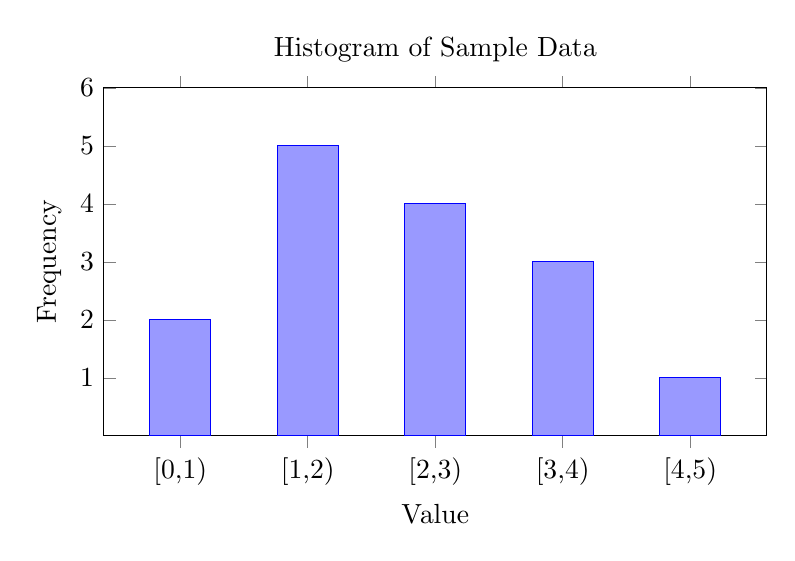
\begin{tikzpicture}
		\pgfplotsset{compat=1.18}
		\begin{axis}[
		    ybar,
		    ymin=0,
		    ymax=6,
		    bar width=22pt,
		    width=10cm,
		    height=6cm,
		    xlabel={Value},
		    ylabel={Frequency},
		    ytick={1,2,3,4,5,6},
		    xtick={1,2,3,4,5},
		    xticklabels={{[0,1)}, {[1,2)}, {[2,3)}, {[3,4)}, {[4,5)}},
		    enlarge x limits=0.15,
		    title={Histogram of Sample Data}
			]
		\addplot+[fill=blue!40] coordinates {(1,2) (2,5) (3,4) (4,3) (5,1)};
		\end{axis}
		\end{tikzpicture}
		\caption{A histogram representing the frequency of \glspl{datapoint} falling within discrete value ranges (i.e., bins). Each bar height shows the count of \gls{sample}s in the corresponding interval.}
		\label{fig:histogram}
		\end{figure}
		See also: \gls{dataset}, \gls{datapoint}, \gls{sample}.
	},
	first={histogram},text={histogram}  
}

\newglossaryentry{bootstrap}
{name={bootstrap},
	description={For\index{bootstrap} the analysis of \gls{ml} methods, it is often useful to interpret 
		a given set of \gls{datapoint}s $\dataset = \big\{ \datapoint^{(1)},\ldots,\datapoint^{(\samplesize)}\big\}$ 
		as \gls{realization}s of \gls{iid} \gls{rv}s with a common \gls{probdist} $p(\datapoint)$. In general, we 
		do not know $p(\datapoint)$ exactly, but we need to estimate it. The bootstrap uses the 
		histogram of $\dataset$ as an estimator for the underlying \gls{probdist} $p(\datapoint)$. 
	},
	first={bootstrap},text={bootstrap}  
}

\newglossaryentry{featurespace}
{name={feature space},
	description={
		The\index{feature space} \gls{feature} space of a given \gls{ml} application or method is 
		constituted by all potential values that the \gls{featurevec} of a \gls{datapoint} can 
		take on. A widely used choice for the \gls{feature} space is the \gls{euclidspace} $\mathbb{R}^{\featuredim}$, 
		with the dimension $\featurelen$ being the number of individual \gls{feature}s of a \gls{datapoint}.},
	first={feature space},text={feature space}  
}


\newglossaryentry{missingdata}
{name={missing data},
	description={Consider\index{missing data} a \gls{dataset} constituted by \gls{datapoint}s collected via 
		some physical \gls{device}. Due to imperfections and failures, some of the \gls{feature} 
		or \gls{label} values of \gls{datapoint}s might be corrupted or simply missing. 
		\Gls{data} imputation aims at estimating these missing values \cite{Abayomi2008DiagnosticsFM}. 
		We can interpret \gls{data} imputation as an \gls{ml} problem where the \gls{label} of a \gls{datapoint} is 
		the value of the corrupted \gls{feature}. },
	first={missing data},text={missing data}  
}


\newglossaryentry{psd}
{name={positive semi-definite (psd)},
	description=
	{A\index{positive semi-definite (psd)} (real-valued) symmetric matrix $\mQ = \mQ^{T} \in \mathbb{R}^{\featuredim \times \featuredim}$ 
	 is referred to as psd if $\featurevec^{T} \mQ \featurevec \geq 0$ for every vector $\featurevec \in \mathbb{R}^{\featuredim}$. 
	 The property of being psd can be extended from matrices to (real-valued) 
	 symmetric \gls{kernel} maps $\kernel: \featurespace \times \featurespace \rightarrow \mathbb{R}$ 
	 (with $\kernel(\featurevec,\featurevec') = \kernel(\featurevec',\featurevec)$)
	 as follows: For any finite set of \gls{featurevec}s $\featurevec^{(1)},\dots,\featurevec^{(\samplesize)}$, 
	 the resulting matrix $\mQ \in \mathbb{R}^{\samplesize \times \samplesize}$ with 
	entries $Q_{\sampleidx,\sampleidx'} = \kernelmap{\featurevec^{(\sampleidx)}}{\featurevec^{(\sampleidx')}}$ 
	is psd \cite{LearningKernelsBook}.},
	first={positive semi-definite (psd)},text={psd}  
}

\newglossaryentry{feature}
{name={caratteristica}, plural={caratteristiche},
	description={Una \index{caratteristica} caratteristica di un \gls{datapoint} è una delle sue proprietà 
		che può essere misurata o calcolata facilmente senza la necessità di supervisione umana. Per esempio, se un \gls{datapoint} 
		è un'immagine digitale (memorizzata, ad esempio, come file \texttt{.jpeg} file), è possibile allora utilizzare le intensità dei canali rosso, 
		verde e blu dei pixel come caratteristiche.Sinonimi del termine feature, specifici del dominio, includono: "covariata", "variabile esplicativa", 
		"variabile indipendente", "variabile di input", "predittore" o "regressore".\cite{Gujarati2021}, \cite{Dodge2003}, \cite{Everitt2022}. 
		}, first={caratteristica}, firstplural={caratteristiche}, text={caratteristica}  
}

\newglossaryentry{featurevec}
{name={vettore delle caratteristiche}, plural = {vettori delle caratteristiche},
	description={Il vettore delle \glspl{feature} si riferisce a\index{vettore delle caratteristiche} un vettore $\vx = \big(x_{1},\ldots,x_{\nrfeatures}\big)^{T}$ 
	i cui elementi sono singole \glspl{feature} $x_{1},\ldots,x_{\nrfeatures}$. Molti metodi di \gls{ml}  
	utilizzano vettori delle \glspl{feature} appartenenti ad uno \gls{euclidspace} di dimensione finita $\mathbb{R}^{\nrfeatures}$. 
	Tuttavia, per alcuni metodi di \gls{ml}, risulta preferibile utilizzare vettori delle \glspl{feature} che risiedono
	 in uno spazio vettoriale di dimensione infinita (si veda, ad esempio, \gls{kernelmethod}). 
		}, 
		first={vettore delle caratteristiche},text={vettore delle caratteristiche}  
}


\newglossaryentry{label}
{name={etichetta}, plural={etichette},
	description={Un'\index{etichetta} informazione o una quantità di livello superiore associata a un \gls{datapoint}.
		Ad esempio, se il \gls{datapoint} è un'immagine, l'etichetta potrebbe indicare se l'immagine contiene o meno un gatto.
		Sinonimi di etichetta, comunemente utilizzati in ambiti specifici, 
		includono variabile di risposta, variabile di output, label e target. \cite{Gujarati2021}, \cite{Dodge2003}, \cite{Everitt2022}.
 },
	first={etichetta},text={etichetta}  
}


\newglossaryentry{data}
{name={dati},
	 description={Con dati\index{dati} ci si riferisce ad oggetti che veicolano informazione. Tali 
	 	oggetti possono essere entità fisiche concrete (come persone o animali), 
		oppure concetti astratti (come i numeri). Spesso si utilizzano rappresentazioni 
		(o approssimazioni) dei dati originari che risultano più convenienti ai fini dell’elaborazione.
	 	Queste approssimazioni si basano su diversi modelli di dati, 
		tra cui il modello relazionale rappresenta uno dei più comunemente adottati. \cite{codd1970relational}.}, 
	text={dati}
}

\newglossaryentry{dataset}
{name={dataset},
	description={A\index{dataset} dataset refers to a collection of \gls{datapoint}s. These 
		\gls{datapoint}s carry information about some quantity of interest (or \gls{label}) within 
		a \gls{ml} application. \gls{ml} methods use datasets for \gls{model} training (e.g., via \gls{erm})
		and \gls{model} \gls{validation}. Note that our notion of a dataset is very flexible as 
		it allows for very different types of \gls{datapoint}s. Indeed, \gls{datapoint}s can be concrete 
		physical objects (such as humans or animals) or abstract objects (such as numbers). 
		As a case in point, Figure\ \ref{fig_cows_dataset} depicts a dataset that consists of cows as 
		\gls{datapoint}s. 
		\begin{figure}[H]
				\begin{center}
		\label{fig:cowsintheswissalps}
		\includegraphics[width=0.5\textwidth]{assets/Cows_in_the_Swiss_Alps}
		  \end{center}
		\caption{\label{fig_cows_dataset}“Cows in the Swiss Alps” by User:Huhu Uet is licensed under [CC BY-SA 4.0](https://creativecommons.org/licenses/by-sa/4.0/)}
	  \end{figure}
       Quite often, an \gls{ml} engineer does not have direct access to a dataset. Indeed, accessing the 
       dataset in Figure\ \ref{fig:cowsintheswissalps} would require to visit the cow herd in the Alps. Instead, 
       we need to use an approximation (or representation) of the dataset which is more convenient 
       to work with. Different mathematical models have been developed for the representation (or approximation) 
       of datasets \cite{silberschatz2019database}, \cite{abiteboul1995foundations}, \cite{hoberman2009data}, \cite{ramakrishnan2002database}. 
       One of the most widely adopted data \gls{model} is the relational model, which organizes \gls{data} 
       as a table (or relation) \cite{codd1970relational}, \cite{silberschatz2019database}.
		A table consists of rows and columns:
		\begin{itemize} 
		\item Each row of the table represents a single \gls{datapoint}.
		\item Each column of the table corresponds to a specific attribute of the \gls{datapoint}. 
		\gls{ml} methods can use attributes as \gls{feature}s and \gls{label}s of the \gls{datapoint}.
		\end{itemize}
		For example, Table \ref{tab:cowdata} shows a representation of the dataset in Figure\ \ref{fig_cows_dataset}. 
		In the relational \gls{model}, the order of rows is irrelevant, and each attribute (i.e., column) must be 
		precisely defined with a domain, which specifies the set of possible values. In \gls{ml} applications, 
		these attribute domains become the \gls{featurespace} and the \gls{labelspace}.
		\begin{table}[H]
			\centering
			\begin{tabular}{lcccc}
				\hline
				\textbf{Name} & \textbf{Weight} & \textbf{Age} & \textbf{Height} & \textbf{Stomach temp} \\
				\hline
				Zenzi & 100 & 4 & 100 & 25 \\
				Berta & 140 & 3 & 130 & 23 \\
				Resi  & 120 & 4 & 120 & 31 \\
				\hline
			\end{tabular}
			\caption{A relation (or table) that represents the dataset in Figure\ \ref{fig:cowsintheswissalps}.}
			\label{tab:cowdata}
		\end{table}
 While the relational model is useful for the study of many \gls{ml} applications, it may be 
 insufficient regarding the requirements for \gls{trustAI}. Modern 
 approaches like datasheets for datasets provide more comprehensive 
 documentation, including details about the dataset’s collection process, intended 
 use, and other contextual information \cite{DatasheetData2021}.},first={dataset},text={dataset}  
}

\newglossaryentry{predictor}
{name={predictor},
	description={A\index{predictor} predictor is a real-valued \gls{hypothesis} map. 
		Given a \gls{datapoint} with \gls{feature}s $\featurevec$, the value 
		$\hypothesis(\featurevec) \in \mathbb{R}$ is used as a \gls{prediction} for the true 
		numeric \gls{label} $\truelabel \in \mathbb{R}$ of the \gls{datapoint}. },first={predictor},text={predictor}  
}

\newglossaryentry{labeled datapoint}
{name={labeled datapoint},
 description={A\index{labeled datapoint} \gls{datapoint} whose \gls{label} is known or has been determined 
 	by some means which might require human labor.},
 first={labeled datapoint},text={labeled datapoint}  
}

\newglossaryentry{rv}
{name={variabile aleatoria}, plural={variabili aleatorie},
 description={Una variabile aleatoria\index{variabile aleatoria} è una \gls{function} che mappa da uno
 	\gls{probspace} $\mathcal{P}$ ad uno spazio dei valori \cite{BillingsleyProbMeasure}, \cite{GrayProbBook}. 
 	Lo \gls{probspace} è costituito da eventi elementari ed è dotato di una misura di \gls{probability} 
 	che assegna \gls{probability} a sottoinsiemi di $\mathcal{P}$. 
 	Diverse tipologie di variabili aleatorie includono:  
 	\begin{itemize} 
 	\item {variabili aleatorie binarie}, che mappano ciascun evento elementare ad un elemento di un insieme binario (ad esempio, $\{-1,1\}$ oppure $\{\text{cat}, \text{no cat}\}$); 
 	\item {variabili aleatorie a valori reali}, che assumono valori nei numeri reali $\mathbb{R}$;  
 	\item {variabili aleatorie a valori vettoriali}, che associano eventi elementari allo \gls{euclidspace} $\mathbb{R}^{\featuredim}$.  
 	\end{itemize} 
 	La teoria della \gls{probability} utilizza il concetto di spazi misurabili per definire in modo rigoroso 
	e studiare le proprietà di collezioni (anche numerose) di variabili aleatorie \cite{BillingsleyProbMeasure}.
			\\
		Si veda anche: \gls{function}, \gls{probspace}, \gls{probability}, \gls{euclidspace}.}, first={variabile aleatoria}, firstplural={variabili aleatorie}, text={variabile aleatoria}  }
 
 \newglossaryentry{probspace}{
 	name={spazio di probabilità}, plural={spazi di probabilità}
 	description={Uno\index{spazio di probabilità} spazio di \gls{probability} è un 
 		\gls{model} matematico di un processo fisico (un esperimento aleatorio) con esito incerto. 
 	   Formalmente, uno spazio di \gls{probability} $\mathcal{P}$ è una terna $(\Omega, \mathcal{F}, P)$ dove:
 		\begin{itemize} 
 		\item  $\Omega$ è lo spazio campionario, che contiene tutti i possibili esiti elementari di un esperimento aleatorio;
 		\item  $\mathcal{F}$ è una sigma-algebra, ovvero una collezione di sottoinsiemi di $\Omega$ (detti eventi) che soddisfa
		determinate proprietà di chiusura rispetto alle operazioni insiemistiche;
 		\item $P$ è una misura di \gls{probability}, cioè una funzione che assegna una \gls{probability} $P(\mathcal{A}) \in [0,1]$ 
 		a ciascun evento $\mathcal{A} \in \mathcal{F}$. Tale funzione deve soddisfare $P(\Omega) = 1$ e 	$
 		P\left(\bigcup_{i=1}^{\infty} \mathcal{A}_i\right) = \sum_{i=1}^{\infty} P(\mathcal{A}_i)$ per ogni 
		successione numerabile di eventi a due a due disgiunti $\mathcal{A}_1, \mathcal{A}_2, \dots$ in $\mathcal{F}$.
 		\end{itemize}
 		Gli spazi di \gls{probability} rappresentano il fondamento teorico per la definizione delle \glspl{rv} e per trattare l’incertezza 
		all’interno delle applicazioni di \gls{ml} \cite{BillingsleyProbMeasure,GrayProbBook,ross2013first}.},  
 	first={spazio di probabilità}, 
 	text={spazio di probabilità}
 }
 
	
\newglossaryentry{realization}
{name={realizzazione}, plural={realizzazioni},
	description={Si consideri\index{realizzazione} una \gls{rv} $x$ che associa a 
	ciascun elemento (ossia, esito o evento elementare) $\omega \in \mathcal{P}$ di uno \gls{probspace} $\mathcal{P}$ 
	ad un elemento $a$ di uno spazio misurabile $\mathcal{N}$ \cite{RudinBookPrinciplesMatheAnalysis}, \cite{HalmosMeasure}, \cite{BillingsleyProbMeasure}. 
	Una realizzazione di $x$ è un qualunque elemento $a' \in \mathcal{N}$ per il quale si ha 
	$x(\omega') = a'$ per qualche $\omega' \in \mathcal{P}$.
			\\
		Si veda anche: \gls{rv}, \gls{probspace}.}, first={realizzazione}, firstplural={realizzazioni},text={realizzazione}  }

\newglossaryentry{trainset}
{name={insieme di addestramento}, plural={insiemi di addestramento},
description={Un\index{insieme di addestramento} insieme di addestramento è un \gls{dataset} $\dataset$ che consiste di alcuni \glspl{datapoint} utilizzati nell'ambito della \gls{erm} 
	per apprendere un'\gls{hypothesis} $\learnthypothesis$. La \gls{loss} media di $\learnthypothesis$ sull' 
	insieme di addestramento è indicata come \gls{trainerr}. Il confronto tra l'\gls{trainerr} e l' 
	\gls{valerr} di $\learnthypothesis$ consente di diagnosticare il metodo di \gls{ml} e fornisce indicazioni su come migliorare  
	l'\gls{valerr} (ad esempio, usando uno \gls{hypospace} diverso o raccogliendo un numero maggiore di \glspl{datapoint}) \cite[Sec. 6.6]{MLBasics}.
			\\
		Si veda anche: \gls{dataset}, \gls{datapoint}, \gls{erm}, \gls{hypothesis}, \gls{loss}, \gls{trainerr}, \gls{valerr}, \gls{ml}, \gls{hypospace}.},first={insieme di addestramento},text={insieme di addestramento}  
}

\newglossaryentry{netmodel}
{name={networked model},
  description={A\index{networked model} networked \gls{model} over an \gls{empgraph} $\graph = \pair{\nodes}{\edges}$ assigns 
   a \gls{localmodel} (i.e., a \gls{hypospace}) to each node $\nodeidx \in \nodes$ of the \gls{empgraph} $\graph$.}, 
   first={networked model},text={networked model}  
}

\newglossaryentry{batch}
{name={batch},
 description={In\index{batch} the context of \gls{stochGD}, a batch refers to a randomly 
	chosen subset of the overall \gls{trainset}. We use the \glspl{datapoint} in this subset 
	to estimate the \gls{gradient} of \gls{trainerr} and, in turn, to update the \gls{modelparams}.
			\\
		See also: \gls{stochGD}, \gls{trainset}, \gls{datapoint}, \gls{gradient}, \gls{trainerr}, \gls{modelparams}.}, 
 first={batch},
 firstplural={batches}, 
 plural={batches}, 
 text={batch}  
}

\newglossaryentry{netdata}
{name={networked data},
	description={Networked\index{networked data} \gls{data} consists of \glspl{localdataset} 
	that are related by some notion of pairwise similarity. We can represent networked 
	\gls{data} using a \gls{graph} whose nodes carry \glspl{localdataset} and edges encode 
	pairwise similarities. One example of networked \gls{data} arises in \gls{fl} applications 
	where \glspl{localdataset} are generated by spatially distributed \glspl{device}.
			\\
		See also: \gls{data}, \gls{localdataset}, \gls{graph}, \gls{fl}, \gls{device}.}, 
	first={networked data},
	text={networked data}  
}

\newglossaryentry{trainerr}
{
	name={errore di addestramento},
	description={La\index{errore di addestramento} \gls{loss} media di una \gls{hypothesis} nel 
		predire le \glspl{label} di un \glspl{datapoint} in un \gls{trainset}. 
		Talvolta, con il termine errore di addestramento ci si riferisce anche alla minima \gls{loss} 
		media ottenuta da una soluzione del problema di \gls{erm}.
				\\
		Si veda anche: \gls{loss}, \gls{hypothesis}, \gls{label}, \gls{datapoint}, \gls{trainset}, \gls{erm}.},
		first={errore di addestramento},text={errore di addestramento}  
}

\newglossaryentry{datapoint}
{name={punto dati}, plural={punti dati},
description={Si definisce \index{punto dati} punto \gls{data} qualsiasi oggetto che contiene o veicola informazione \cite{coverthomas}. Possono essere punti \gls{data}  
		studenti, segnali radio, alberi, foreste, immagini, \gls{rv}s, numeri reali o proteine. I punti \gls{data} si caratterizzano 
		utilizzando due tipologie di proprietà. Un tipo di proprietà sono le \glspl{feature}. \Glspl{feature} sono proprietà di un 
		punto \gls{data} che possono essere misurate o calcolate in modo automatico. 
		Un secondo tipo di proprietà viene definita \gls{label}. L' \gls{label} di 
		un punto \gls{data} rappresenta un'informazione di livello superiore (o una quantità di interesse). 
		A differenza delle \glspl{feature}, la determinazione dell’ \gls{label} di un punto \gls{data} trichiede tipicamente l’intervento di esperti umani (esperti del dominio). 
		In termini generali, l’obiettivo del \gls{ml} è quello di prevedere 
		l' \gls{label} di un punto \gls{data} basandosi esclusivamente sulle sue \glspl{feature}. 
				\\
		See also: \gls{data}, \gls{rv}, \gls{feature}, \gls{label}, \gls{ml}.
		}, first={punto dati},text={punto dati}  
}


\newglossaryentry{valerr}
{name={errore di validazione}, plural={errori di validazione},
 description={Si consideri\index{errore di validazione} una \gls{hypothesis} $\learnthypothesis$ ottenuta 
 mediante un qualche metodo di \gls{ml}, ad esempio utilizzando la \gls{erm} su un \gls{trainset}. La \gls{loss} media
 	di $\learnthypothesis$ su un \gls{valset}, distinto dal \gls{trainset}, è detta
 	errore di \gls{validation}.
			\\
		Si veda anche: \gls{hypothesis}, \gls{ml}, \gls{erm}, \gls{trainset}, \gls{loss}, \gls{valset}, \gls{validation}.},
		first={errore di validazione},text={errore di validazione}  
}

\newglossaryentry{validation} 
{name={validazione},
	description={Si consideri\index{validation} una \gls{hypothesis} $\learnthypothesis$ appresa mediante 
	qualche metodo di \gls{ml},ad esempio risolvendo un problema di \gls{erm} su un \gls{trainset} $\dataset$. 
		La validazione si riferisce alla pratica di valutare la \gls{loss} associata alla 
		\gls{hypothesis} $\learnthypothesis$ su un insieme di
		\glspl{datapoint} che non appartengono all'\gls{trainset} $\dataset$.
				\\
		Si veda anche: \gls{hypothesis}, \gls{ml}, \gls{erm}, \gls{trainset}, \gls{loss}, \gls{datapoint}. },first={validazione},text={validazione}  
}

\newglossaryentry{quadfunc}
{name={quadratic function},
	description={A\index{quadratic function} \gls{function} $f: \mathbb{R}^{\nrfeatures} \rightarrow \mathbb{R}$ of the form 
	$$f(\weights) =  \weights^{T} \mathbf{Q} \mathbf{w} + \mathbf{q}^{T} \weights+a,$$ with 
	some matrix $\mQ \in \mathbb{R}^{\nrfeatures \times \nrfeatures}$, vector $\vq \in \mathbb{R}^{\nrfeatures}$, 
	and scalar $a \in \mathbb{R}$.
	\\
	See also: \gls{function}. },first={quadratic function},text={quadratic function}  
}

\newglossaryentry{valset}
{name={insieme di validazione},
  description={Un\index{insieme di validazione} insieme di \glspl{datapoint} utilizzato per stimare 
  il \gls{risk} di una \gls{hypothesis} $\learnthypothesis$ appresa mediante un metodo di 
  	\gls{ml} (ad esempio, risolvendo il problema di \gls{erm}). La \gls{loss} media di $\learnthypothesis$ 
  	sull'insieme di \gls{validation} è indicata come \gls{valerr} e può essere utilizzata per diagnosticare un metodo di 
  	\gls{ml} (si veda \cite[Sec. 6.6]{MLBasics}). Il confronto tra \gls{trainerr} 
  	e \gls{valerr} può fornire indicazioni utili per il miglioramento del metodo di \gls{ml} (come ad esempio l'impiego di un 
	diverso \gls{hypospace}).
			\\
		Si veda anche: \gls{datapoint}, \gls{risk}, \gls{hypothesis}, \gls{ml}, \gls{erm}, \gls{loss}, \gls{validation}, \gls{valerr}, \gls{trainerr}, \gls{hypospace}.},first={insieme di validazione},text={insieme di validazione}  
}

\newglossaryentry{testset}
{name={test set},
	description={A\index{test set} set of \glspl{datapoint} that have  
		been used neither to train a \gls{model} (e.g., via \gls{erm}) nor in a \gls{valset} 
		to choose between different \glspl{model}.
				\\
		See also: \gls{datapoint}, \gls{model}, \gls{erm}, \gls{valset}.},first={test set},text={test set}  
}


\newglossaryentry{modelsel}
{name={model selection},
	description={In\index{model selection} \gls{ml}, \gls{model} selection refers to the 
		process of choosing between different candidate \gls{model}s. In its most 
		basic form, \gls{model} selection amounts to: 1) training each candidate \gls{model}; 
		2) computing the \gls{valerr} for each trained \gls{model}; and 3) choosing the \gls{model} 
		with the smallest \gls{valerr} \cite[Ch. 6]{MLBasics}. },first={model selection},text={model selection}  
}





\newglossaryentry{linclass}{name={linear classifier}, description={
	    Consider\index{linear classifier} \gls{datapoint}s characterized by numeric \gls{feature}s $\featurevec \in \mathbb{R}^{\nrfeatures}$ 
	    and a \gls{label} $\truelabel \in \labelspace$ from some finite \gls{labelspace} $\labelspace$. 
		A linear \gls{classifier} is characterized by having \gls{decisionregion}s that are 
		separated by hyperplanes in $\mathbb{R}^{\featuredim}$ \cite[Ch. 2]{MLBasics}.},first={linear classifier},text={linear classifier} }

\newglossaryentry{erm}{name={empirical risk minimization (ERM)}, description={\Gls{emprisk} minimization\index{empirical risk minimization (ERM)} is the optimization problem of finding 
		a \gls{hypothesis} (out of a \gls{model}) with the \gls{minimum} average \gls{loss} (or \gls{emprisk}) on a given \gls{dataset} 
		$\dataset$ (i.e., the \gls{trainset}). Many \gls{ml} methods are obtained from 
		\gls{emprisk} via specific design choices for the \gls{dataset}, \gls{model}, and \gls{loss} \cite[Ch. 3]{MLBasics}.},
	first={empirical risk minimization (ERM)},text={ERM} }

\newglossaryentry{multilabelclass}{name={multi-label classification}, description={Multi-\gls{label} 
		\gls{classification}\index{multi-label classification} problems and methods use \gls{datapoint}s 
		that are characterized by several \gls{label}s. As an example, consider a \gls{datapoint} 
		representing a picture with two \gls{label}s. One \gls{label} indicates the presence of a human 
		in this picture and another \gls{label} indicates the presence of a car.},
	    first={multi-label classification},text={multi-label classification} }


\newglossaryentry{ssl}{name={semi-supervised learning (SSL)}, description={SSL\index{semi-supervised learning (SSL)} 
		methods use unlabeled datapoints to support the learning of a \gls{hypothesis} 
		from \gls{labeled datapoint}s \cite{SemiSupervisedBook}. This approach is particularly useful 
		for \gls{ml} applications that offer a large amount of unlabeled datapoints, but only a limited 
		number of \gls{labeled datapoint}s.}, 
		first={semi-supervised learning (SSL)},text={SSL} }
	
	
\newglossaryentry{objfunc}{name={objective function}, description={An\index{objective function} 
		objective function is a map that assigns each value of an optimization variable, such 
		as the \gls{modelparams} $\weights$ of a \gls{hypothesis} $\hypothesis^{(\weights)}$, to 
		an objective value $f(\weights)$. The objective value $f(\weights)$ could be the 
		\gls{risk} or the \gls{emprisk} of a \gls{hypothesis} $\hypothesis^{(\weights)}$.},first={objective function},text={objective function} }
	
\newglossaryentry{regularizer}{name={regularizer}, description={A regularizer\index{regularizer} 
		assigns each \gls{hypothesis} $\hypothesis$ from a \gls{hypospace} $\hypospace$ a quantitative 
		measure $\regularizer{\hypothesis}$ for how much its \gls{prediction} error on a \gls{trainset} might 
		differ from its \gls{prediction} errors on \gls{datapoint}s outside the \gls{trainset}. \Gls{ridgeregression} 
		uses the regularizer $\regularizer{\hypothesis} \defeq \normgeneric{\weights}{2}^{2}$ for linear \gls{hypothesis} maps $\hypothesis^{(\weights)}(\featurevec) \defeq \weights^{T} \featurevec$ \cite[Ch. 3]{MLBasics}. 
		\Gls{lasso} uses the regularizer $\regularizer{\hypothesis} \defeq \normgeneric{\weights}{1}$ 
		for linear \gls{hypothesis} maps $\hypothesis^{(\weights)}(\featurevec) \defeq \weights^{T} \featurevec$ \cite[Ch. 3]{MLBasics}. },first={regularizer},text={regularizer} }


\newglossaryentry{regularization}{name={regularization}, description={
		A\index{regularization} key challenge of modern \gls{ml} applications is that they often 
		use large \gls{model}s, which have an \gls{effdim} in the order of billions. 
		Training a high-dimensional \gls{model} using basic \gls{erm}-based methods
		is prone to \gls{overfitting}: the learned \gls{hypothesis} performs well on the \gls{trainset} 
		but poorly outside the \gls{trainset}. Regularization refers to modifications of a given instance 
		of \gls{erm} in order to avoid \gls{overfitting}, i.e., to ensure that the learned \gls{hypothesis} performs 
		not much worse outside the \gls{trainset}. There are three routes for implementing 
		regularization: 
		\begin{enumerate}[label=\arabic*)]
			\item {\Gls{model} pruning:} We prune the original \gls{model} $\hypospace$ to obtain a 
			smaller \gls{model} $\hypospace'$. For a parametric \gls{model}, the pruning can be 
			implemented via constraints on the \gls{modelparams} (such as $w_{1} \in [0.4,0.6]$ for 
			the weight of \gls{feature} $x_{1}$ in \gls{linreg}).
			\item {\Gls{loss} penalization:} We modify the \gls{objfunc} of \gls{erm} by adding a 
			penalty term to the \gls{trainerr}. The penalty term estimates how much larger the expected \gls{loss} (or \gls{risk}) 
			is compared to the average \gls{loss} on the \gls{trainset}. 
			\item {\Gls{dataaug}:} We can enlarge the \gls{trainset} $\dataset$ by adding 
			perturbed copies of the original \gls{datapoint}s in $\dataset$. One example for such 
			a perturbation is to add the \gls{realization} of an \gls{rv} to the \gls{featurevec} 
			of a \gls{datapoint}. 
		\end{enumerate} 
		Figure \ref{fig_equiv_dataaug_penal_dict} illustrates the above three routes to regularization. 
		These routes are closely related and sometimes fully equivalent: \gls{dataaug} using \gls{gaussrv}s 
		to perturb the \gls{featurevec}s in the \gls{trainset} of \gls{linreg} 
		has the same effect as adding the penalty 
		$\lambda \normgeneric{\weights}{2}^2$ to the \gls{trainerr} (which is nothing but \gls{ridgeregression}). 
        The decision on which route to use for regularization can be based on the 
        available computational infrastructure. For example, it might be much easier to 
        implement \gls{dataaug} than \gls{model} pruning. 
		\begin{figure}[H]
			\begin{center} 
				\begin{tikzpicture}[scale = 1]
					% Axes
					\draw[->, very thick] (0,0.5) -- (7.7,0.5) node[right] {\gls{feature} $\feature$};       % X-axis
					\draw[->, very thick] (0.5,0) -- (0.5,4.2) node[above] {\gls{label} $\truelabel$};   % Y-axis
					\draw[color=black, thick, dashed, domain = -1: 6.2, variable = \x]  plot ({\x},{\x*0.4 + 2.0}) ;     
					\draw[color=black, thick, dashed, domain = -1: 6.2, variable = \x]  plot ({\x},{\x*0.6 + 2.0}) ;     
					            % Add a lasso around the two dashed lines
	          % Ellipse around the two dashed lines
					\draw[blue, thick] (5, 4.5) ellipse [x radius=0.2cm, y radius=1cm];
					\node at (5, 5.8) [text=black, font=\small] {$\{ \hypothesis: \hypothesis(x)\!=\!w_{1}x\!+\!w_{0}; w_{1} \in [0.4,0.6]\}$};
					\node at (6.7,4.5) {$\hypothesis(\feature)$};    
					\coordinate (l1)   at (1.2, 2.48);
					\coordinate (l2) at (1.4, 2.56);
					\coordinate (l3)   at (1.7,  2.68);
					\coordinate (l4)   at (2.2, 2.2*0.4+2.0);
					\coordinate (l5) at (2.4, 2.4*0.4+2.0);
					\coordinate (l6)   at (2.7,  2.7*0.4+2.0);
					\coordinate (l7)   at (3.9,  3.9*0.4+2.0);
					\coordinate (l8) at (4.2, 4.2*0.4+2.0);
					\coordinate (l9)   at (4.5,  4.5*0.4+2.0);
					\coordinate (n1)   at (1.2, 1.8);
					\coordinate (n2) at (1.4, 1.8);
					\coordinate (n3)   at (1.7,  1.8);
					\coordinate (n4)   at (2.2, 3.8);
					\coordinate (n5) at (2.4, 3.8);
					\coordinate (n6)   at (2.7,  3.8);
					% augemented data point obtained by perturbing feature, not touching label value 
					\coordinate (n7)   at (3.9, 2.6);
					\coordinate (n8) at (4.2, 2.6);
					\coordinate (n9)   at (4.5,  2.6);
					\node at (n1)  [circle,draw,fill=red,minimum size=6pt,scale=0.6, name=c1] {};
					\node at (n2)  [circle,draw,fill=blue,minimum size=6pt, scale=0.6, name=c2] {};
					\node at (n3)  [circle,draw,fill=red,minimum size=6pt,scale=0.6,  name=c3] {};
					\node at (n4)  [circle,draw,fill=red,minimum size=12pt, scale=0.6, name=c4] {};  
					\node at (n5)  [circle,draw,fill=blue,minimum size=12pt,scale=0.6,  name=c5] {};
					\node at (n6)  [circle,draw,fill=red,minimum size=12pt, scale=0.6, name=c6] {};  
					\node at (n7)  [circle,draw,fill=red,minimum size=12pt,scale=0.6,  name=c7] {};
					\node at (n8)  [circle,draw,fill=blue,minimum size=12pt, scale=0.6, name=c8] {};
					\node at (n9)  [circle,draw,fill=red,minimum size=12pt, scale=0.6, name=c9] {};
					\draw [<->] ($ (n7) + (0,-0.3) $)  --  ($ (n9) + (0,-0.3) $) node [pos=0.4, below] {$\sqrt{\regparam}$}; ; 
					\draw[<->, color=red, thick] (l1) -- (c1);  
					\draw[<->, color=blue, thick] (l2) -- (c2);  
					\draw[<->, color=red, thick] (l3) -- (c3);  
					\draw[<->, color=red, thick] (l4) -- (c4);  
					\draw[<->, color=blue, thick] (l5) -- (c5);  
					\draw[<->, color=red, thick] (l6) -- (c6);  
					\draw[<->, color=red, thick] (l7) -- (c7);  
					\draw[<->, color=blue, thick] (l8) -- (c8);  
					\draw[<->, color=red, thick] (l9) -- (c9);  
					\draw[fill=blue] (6.2, 3.7)  circle (0.1cm) node [black,xshift=2.3cm] {original \gls{trainset} $\dataset$};
					\draw[fill=red] (6.2, 3.2)  circle (0.1cm) node [black,xshift=1.3cm] {augmented};
					\node at (4.6,1.2)  [minimum size=12pt, font=\fontsize{12}{0}\selectfont, text=blue] {$\frac{1}{\samplesize} \sum_{\sampleidx=1}^\samplesize \lossfunc{\pair{\featurevec^{(\sampleidx)}}{ \truelabel^{(\sampleidx)}}}{\hypothesis}$};
					\node at (7.8,1.2)  [minimum size=12pt, font=\fontsize{12}{0}\selectfont, text=red] {$+\regparam \regularizer{\hypothesis}$};
				\end{tikzpicture}
				\caption{Three approaches to regularization: 1) \gls{dataaug}; 2) \gls{loss} penalization; and 3) \gls{model} 
				pruning (via constraints on \gls{modelparams}). \label{fig_equiv_dataaug_penal_dict} }
			\end{center}
		\end{figure} 
		\newpage
		},first={regularization},text={regularization} }
	

\newglossaryentry{rerm}{
	name={regularized empirical risk minimization (RERM)}, 
	description={Basic \gls{erm} learns a \gls{hypothesis} (or trains a \gls{model}) $\hypothesis \in \hypospace$ 
		based solely on the \gls{emprisk} $\emprisk{\hypothesis}{\dataset}$ incurred on a \gls{trainset} $\dataset$. 
		To make \gls{erm} less prone to \gls{overfitting}, we can implement \gls{regularization} by 
		including a (scaled) \gls{regularizer} $\regularizer{\hypothesis}$ in the learning objective. 
		This leads to regularized empirical risk minimization (RERM)\index{regularized empirical risk minimization (RERM)}, 
		\begin{equation}
			\label{equ_def_rerm}
			\learnthypothesis \in \argmin_{\hypothesis \in \hypospace} \emprisk{\hypothesis}{\dataset} + \regparam \regularizer{\hypothesis}.
		\end{equation}
		The parameter $\regparam \geq 0$ controls the \gls{regularization} strength. 
		For $\regparam = 0$, we recover standard \gls{erm} without \gls{regularization}. As $\regparam$ increases, the 
		learned \gls{hypothesis} is increasingly biased toward small values of $\regularizer{\hypothesis}$. 
		The component $\regparam \regularizer{\hypothesis}$ in the \gls{objfunc} of \eqref{equ_def_rerm} 
		can be intuitively understood as a surrogate for the increased average \gls{loss} that may 
		occur when predicting \gls{label}s for \gls{datapoint}s outside the \gls{trainset}. This intuition  
		can be made precise in various ways. For example, consider a \gls{linmodel} trained using \gls{sqerrloss} 
		and the \gls{regularizer} $\regularizer{\hypothesis} = \normgeneric{\weights}{2}^{2}$. 
		In this setting, $\regparam \regularizer{\hypothesis}$ corresponds to the expected increase in \gls{loss} 
		caused by adding \gls{gaussrv}s to the \gls{featurevec}s in the \gls{trainset} 
		\cite[Ch. 3]{MLBasics}.
		A principled construction for the \gls{regularizer} $\regularizer{\hypothesis}$ 
		arises from approximate upper bounds on the generalization error. The resulting 
		RERM instance is known as \gls{srm} \cite[Sec. 7.2]{ShalevShwartz2009}.
	}, 
	first={regularized empirical risk minimization (RERM)},
	text={RERM} 
}


\newglossaryentry{generalization}{name={generalization}, 
	description={Many\index{generalization} current \gls{ml} (and \gls{ai}) systems 
		are based on \gls{erm}: At their core, they train a \gls{model} (i.e., learn a \gls{hypothesis} 
		$\learnthypothesis \in \hypospace$) by minimizing the average \gls{loss} (or \gls{emprisk}) on some 
		\gls{datapoint}s $\vz^{(1)},\ldots,\vz^{(\samplesize)}$, which serve as a \gls{trainset} $\trainset$. 
		Generalization refers to an \gls{ml} method's ability to perform well outside the \gls{trainset}. 
		Any mathematical theory of generalization needs some mathematical concept for the 
		"outside the \gls{trainset}." For example, statistical learning theory uses a 
		\gls{probmodel} such as the \gls{iidasspt} for \gls{data} generation: the \gls{datapoint}s in 
		the \gls{trainset} are \gls{iid} \gls{realization}s of some underlying \gls{probdist} $p(\vz)$. 
		A \gls{probmodel} allows us to explore the outside of the \gls{trainset} by 
		drawing additional \gls{iid} \gls{realization}s from $p(\vz)$. Moreover, using the \gls{iidasspt} 
		allows us to define the \gls{risk} of a trained \gls{model} $\learnthypothesis \in \hypospace$ as 
		the expected \gls{loss} $\risk{\learnthypothesis}$. What is more, we can use concentration 
		bounds or convergence results for sequences of \gls{iid} \gls{rv}s to bound the deviation 
		between the \gls{emprisk} $\emprisk{\learnthypothesis}{\trainset}$ of a trained \gls{model} and 
		its \gls{risk} \cite{ShalevMLBook}. It is possible to study generalization also without using 
		\gls{probmodel}s. For example, we could use (deterministic) 
	    perturbations of the \gls{datapoint}s in the \gls{trainset} to study its outside. 
	    In general, we would like the trained \gls{model} to be robust, i.e., its \gls{prediction}s 
	    should not change too much for small perturbations of a \gls{datapoint}. Consider a trained \gls{model} for detecting 
	    an object in a smartphone snapshot. The detection result should not change if we mask a 
	    small number of randomly chosen pixels in the image \cite{OnePixelAttack}. 
		  \begin{figure}[H]
		                   	\centering
		                   	\begin{tikzpicture}[scale=0.8]
 % Filled ellipsoid to represent p(z)
							   \draw[lightblue, fill=lightblue, opacity=0.5] (3, 2) ellipse (6cm and 2cm);
% Label for p(z)
								\node[black] at (6, 3) {$p(z)$};
		                   		% Data points
		                   		\fill[blue] (1, 3) circle (4pt) node[below, xshift=0pt, yshift=0pt] {$\datapoint^{(1)}$};
		                   		\fill[blue] (5, 1) circle (4pt) node[below] {$\datapoint^{(2)}$};
		                   		% Shifted copies for datapoint^{(1)}
		                   		\fill[blue] (1.6, 3) circle (3pt);
		                   		\fill[blue] (0.4, 3) circle (3pt);
		                   		\draw[<->, thin] (1, 3) -- (1.6, 3);
		                   		\draw[<->, thin] (1, 3) -- (0.4, 3);
		                   		% Shifted copies for datapoint^{(2)}
		                   		\fill[blue] (5.6, 1) circle (3pt);
		                   		\fill[blue] (4.4, 1) circle (3pt);
		                   		\draw[<->, thin] (5, 1) -- (5.6, 1);
		                   		\draw[<->, thin] (5, 1) -- (4.4, 1);
		                   		% Polynomial curve
		                   		\draw[black, thick, domain=0:6, smooth] plot (\x, {- 1*\x + 5});
		                   		% Label for polynomial
		                   		\node[black] at (3, 2.5) [right] {$\learnthypothesis$};
		                   	\end{tikzpicture}
		                   	\caption{Two \gls{datapoint}s $\datapoint^{(1)},\datapoint^{(2)}$ that are used as a \gls{trainset} 
		                   		to learn a \gls{hypothesis} $\learnthypothesis$ via \gls{erm}. We can evaluate $\learnthypothesis$ 
		                   		outside $\trainset$ either by an \gls{iidasspt} with some underlying \gls{probdist} $p(\datapoint)$ 
		                   		or by perturbing the \gls{datapoint}s.}
		                   	\label{fig:polynomial_fit_dict}
		                   \end{figure}
		                   \newpage
		},
	first={generalization},text={generalization} }

	
\newglossaryentry{gtv}{name={generalized total variation (GTV)}, description={GTV is a\index{generalized total variation (GTV)} 
		measure of the variation of trained \gls{localmodel}s $\localhypothesis{\nodeidx}$ 
		(or their \gls{modelparams} $\localparams{\nodeidx}$) assigned to the nodes $\nodeidx=1,\ldots,\nrnodes$ 
		of an undirected weighted \gls{graph} $\graph$ with edges $\edges$. Given a measure $\discrepancy{\hypothesis}{\hypothesis'}$ 
		for the \gls{discrepancy} between \gls{hypothesis} maps $\hypothesis,\hypothesis'$, the GTV is 
		\begin{equation} 
			\nonumber
			\sum_{\edge{\nodeidx}{\nodeidx'}\in \edges} \edgeweight_{\nodeidx,\nodeidx'} 
			\discrepancy{\localhypothesis{\nodeidx}}{\localhypothesis{\nodeidx'}}.
		\end{equation}
		Here, $\edgeweight_{\nodeidx,\nodeidx'}>0$ denotes the weight of the undirected edge $\edge{\nodeidx}{\nodeidx'}\in \edges$.
		},first={GTV},text={GTV} }
	
\newglossaryentry{srm}{
	name={structural risk minimization (SRM)},
	description={Structural\index{structural risk minimization (SRM)} risk minimization (SRM) is an 
		instance of \gls{rerm}, which which the \gls{model} $\hypospace$ can be expressed 
		as a countable union of  sub-models: $\hypospace = \bigcup_{n=1}^{\infty} \hypospace^{(n)}$. 
		Each sub-model $\hypospace^{(n)}$ permits the derivation of an approximate upper bound 
		on the generalization error incurred when applying \gls{erm} to train $\hypospace^{(n)}$. 
		These individual bounds—one for each sub-model—are then combined to form a \gls{regularizer} 
		used in the \gls{rerm} objective. 
        These approximate upper bounds (one for each $\hypospace^{(n)}$) are then combined 
		to construct a \gls{regularizer} for \gls{rerm} \cite[Sec.\ 7.2]{ShalevMLBook}.},
		text={SRM}
 }
 
 \newglossaryentry{rlm}{
 	name={regularized loss minimization (RLM)},
 	description={See\index{regularized loss minimization (RLM)} \gls{rerm}.},
 	text={RLM}
 }
 

\newglossaryentry{datapoisoning}{name={data poisoning}, description={\Gls{data}\index{data poisoning} 
		poisoning refers to the intentional manipulation (or fabrication) of \gls{datapoint}s to 
		steer the training of an \gls{ml} \gls{model} \cite{Liu2021,PoisonGAN}. The protection against 
		\gls{data} poisoning is particularly important in distributed \gls{ml} applications where \gls{dataset}s are decentralized.},first={data poisoning},text={data poisoning} }
	
	
\newglossaryentry{backdoor}{name={backdoor}, description={A\index{backdoor} backdoor attack refers 
		to the intentional manipulation of the training process underlying an \gls{ml} method. This manipulation 
		can be implemented by perturbing the \gls{trainset} (\gls{data} poisoning) or the 
		optimization \gls{algorithm} used by an \gls{erm}-based method. The goal of a 
		backdoor attack is to nudge the learned \gls{hypothesis} $\learnthypothesis$ 
		towards specific \gls{prediction}s for a certain range of \gls{feature} values. This range of \gls{feature} 
		values serves as a key (or trigger) to unlock a backdoor in the sense of 
		delivering anomalous \gls{prediction}s. The key $\featurevec$ and the corresponding 
		anomalous \gls{prediction} $\learnthypothesis(\featurevec)$ are only known to the attacker.},
	first={backdoor},text={backdoor} }


\newglossaryentry{clustasspt}{name={clustering assumption}, description={The\index{clustering assumption} 
		\gls{clustering} assumption postulates that \gls{datapoint}s in a \gls{dataset} form a (small) number of 
		groups or clusters. \Gls{datapoint}s in the same \gls{cluster} are more similar to each 
		other than those outside the \gls{cluster} \cite{SemiSupervisedBook}. We obtain different 
		\gls{clustering} methods by using different notions of similarity between \gls{datapoint}s.},first={clustering assumption},text={clustering assumption} }
	
\newglossaryentry{dosattack}{name={denial-of-service attack}, description={A\index{denial-of-service attack} 
		denial-of-service attack aims (e.g., via \gls{datapoisoning}) to steer the training of a \gls{model} 
		such that it performs poorly for typical \gls{datapoint}s.},
	first={denial-of-service attack},text={denial-of-service attack} }

\newglossaryentry{netexpfam}{name={networked exponential families (nExpFam)}, 
	description={A\index{networked exponential families (nExpFam)} collection of exponential 
		families, each of them assigned to a node of an \gls{empgraph}. The \gls{modelparams} are coupled 
	   via the network structure by requiring them to have a small \gls{gtv} \cite{JungNetExp2020}. },first={networked exponential family (nExpFam)},text={nExpFam} }
	 


\newglossaryentry{scatterplot}{name={diagramma a dispersione}, description={Una\index{diagramma a dispersione} 
		tecnica di visualizzazione che rappresenta i \glspl{datapoint} su un piano bidimensionale utilizzando degli indicatori.
		La Figura \ref{fig_scatterplot_temp_FMI_dict} mostra un esempio di diagramma a dispersione.  
		\begin{figure}[H]
			\begin{center}
				\begin{tikzpicture}[scale=1]
					\tikzset{x=2cm,y=2cm,every path/.style={>=latex},node style/.style={circle,draw}}
					\begin{axis}[axis x line=none,
						axis y line=none,
						ylabel near ticks,
						xlabel near ticks,
						enlarge y limits=true,
						xmin=-5, xmax=30,
						ymin=-5, ymax=30,
						width=6cm, height=6cm ]
						\addplot[only marks] table [x=mintmp, y=maxtmp, col sep = semicolon] {assets/FMIData1.csv};
						\node at (axis cs:26,2) [anchor=west] {$\feature$};
						\node at (axis cs:0,30) [anchor=west] {$\truelabel$};
						\draw[->] (axis cs:-5,0) -- (axis cs:30,0);
						\draw[->] (axis cs:0,-5) -- (axis cs:0,30);
					\end{axis}
				\end{tikzpicture}
				\vspace*{-10mm}
			\end{center}
			\caption{Un diagramma a dispersione con indicatori circolari, in cui i \glspl{datapoint} rappresentano le condizioni 
			meteorologiche giornaliere in Finlandia.
				Ogni \gls{datapoint} ë caratterizzato dalla sua temperatura \gls{minimum} diurna $\feature$ 
				come \gls{feature} e dalla sua temperatura \gls{maximum} diurna $\truelabel$ come \gls{label}. 
				Le temperature sono state misurate presso la stazione meteorologica \gls{fmi} di Helsinki Kaisaniemi, 
				nel periodo compreso tra il 1.9.2024 e il 28.10.2024.}
			\label{fig_scatterplot_temp_FMI_dict}
			\vspace*{-3mm}
			\end{figure}
		Un diagramma a dispersione può rendere possibile l’ispezione visiva dei \glspl{datapoint}, i quali sono, per loro natura, 
		rappresentati dai \glspl{featurevec} in spazi ad alta dimensionalità.\\
		Si veda anche: \gls{datapoint}, \gls{minimum}, \gls{feature}, \gls{maximum}, \gls{label}, \gls{fmi}, \gls{featurevec}, \gls{dimred}.
		},first={diagramma a dispersione},plural={diagrammi a dispersione},text={diagramma a dispersione} }


\newglossaryentry{stepsize}{name={step size}, description={
		See\index{step size} \gls{learnrate}.}, 
	first={step size},text={step size} }

\newglossaryentry{learnrate}{name={learning rate}, description={Consider\index{learning rate} 
		an iterative \gls{ml} method for finding or learning a useful \gls{hypothesis} $\hypothesis \in \hypospace$. 
		Such an iterative method repeats similar computational (update) steps that adjust or 
		modify the current \gls{hypothesis} to obtain an improved \gls{hypothesis}. One 
		well-known example of such an iterative learning method is \gls{gd} and its variants, \gls{stochGD} and 
		\gls{projgd}. A key parameter of an iterative method is the learning rate. 
		The learning rate controls the extent to which the current \gls{hypothesis} 
		can be modified during a single iteration. A well-known example of such a parameter 
		is the \gls{stepsize} used in \gls{gd} \cite[Ch. 5]{MLBasics}.},
	first={learning rate},text={learning rate} }

\newglossaryentry{featuremap}{name={feature map}, description={\Gls{feature} map refers to a\index{feature map} map 
		that transforms the original \gls{feature}s of a \gls{datapoint} into new \gls{feature}s. The 
		so-obtained new \gls{feature}s might be preferable over the original \gls{feature}s for 
		several reasons. For example, the arrangement of \gls{datapoint}s might become 
		simpler (or more linear) in the new \gls{featurespace}, allowing the use of \gls{linmodel}s 
		in the new \gls{feature}s. This idea is a main driver for the development of \gls{kernelmethod}s \cite{LearningKernelsBook}. 
		Moreover, the hidden layers of a \gls{deepnet} can be interpreted as a trainable \gls{feature} map 
		followed by a \gls{linmodel} in the form of the output layer. Another reason for learning a \gls{feature} map
		could be that learning a small number of new \gls{feature}s helps to avoid \gls{overfitting} and 
		ensures \gls{interpretability} \cite{Ribeiro2016}. The special case of a \gls{feature} map delivering 
		two numeric \gls{feature}s is particularly useful for \gls{data} visualization. Indeed, we can depict 
		\gls{datapoint}s in a \gls{scatterplot} by using two \gls{feature}s as the coordinates of a \gls{datapoint}.},
	first={feature map},text={feature map} }
	
 
  \newglossaryentry{lasso}{name={least absolute shrinkage and selection operator (Lasso)}, 
	description={The Lasso\index{least absolute shrinkage and selection operator (Lasso)} is an 
		instance of \gls{srm}. It learns the \gls{weights} $\weights$ of a linear map 
		$\hypothesis(\featurevec) = \weights^{T} \featurevec$ based on a \gls{trainset}. 
		Lasso is obtained from \gls{linreg} by adding the scaled $\ell_{1}$-\gls{norm} 
		$\regparam \normgeneric{\weights}{1}$ to the average \gls{sqerrloss} incurred on the \gls{trainset}. 
	},
	first={Lasso},text={Lasso} }
 
 \newglossaryentry{simgraph}{name={similarity graph}, 
 	description={Some\index{similarity graph} \gls{ml} applications generate \gls{datapoint}s that 
 		are related by a domain-specific notion of similarity. These similarities can be 
 		represented conveniently using a similarity \gls{graph} $\graph = \big(\nodes \defeq \{1,\ldots,\samplesize\},\edges\big)$. 
 		The node $\sampleidx \in \nodes$ represents the $\sampleidx$-th \gls{datapoint}. Two 
 		nodes are connected by an undirected edge if the corresponding \gls{datapoint}s are similar. 
 	},
 	first={similarity graph},text={similarity graph} }
 
 
 \newglossaryentry{kld}{name={Kullback-Leibler divergence (KL divergence)}, 
 	description={
 		 The\index{Kullback-Leibler divergence (KL divergence)} KL divergence is a quantitative 
 		 measure of how much one \gls{probdist} is different from another \gls{probdist} \cite{coverthomas}.  
 	},
 	first={Kullback-Leibler divergence (KL divergence)},text={KL divergence} }

\newglossaryentry{LapMat}{
	name={Laplacian matrix},
	description={The\index{Laplacian matrix} structure of a \gls{graph} $\graph$, with 
		nodes $\nodeidx=1,\ldots,\nrnodes$, can be analyzed using the properties of 
		special matrices that are associated with $\graph$. One such matrix is the 
		\gls{graph} Laplacian matrix $\mL^{(\graph)} \in \mathbb{R}^{\nrnodes \times \nrnodes}$, 
		which is defined for an undirected and weighted \gls{graph} \cite{Luxburg2007,Ng2001}. 
		It is defined element-wise as (see Figure \ref{fig_lap_mtx_dict})
	\begin{equation}
		\LapMatEntry{\graph}{\nodeidx}{\nodeidx'} \defeq \begin{cases} - \edgeweight_{\nodeidx,\nodeidx'} & \mbox{ for } \nodeidx\neq \nodeidx', \edge{\nodeidx}{\nodeidx'}\!\in\!\edges, \\ 
			\sum_{\nodeidx'' \neq \nodeidx} \edgeweight_{\nodeidx,\nodeidx''} & \mbox{ for } \nodeidx = \nodeidx', \\ 
							0 & \mbox{ else.} \end{cases}
	 \end{equation}
  Here, $\edgeweight_{\nodeidx,\nodeidx'}$ denotes the \gls{edgeweight} of an edge $\edge{\nodeidx}{\nodeidx'} \in \edges$. 
  \begin{figure}[H]
  	\begin{center}
    \begin{minipage}{0.45\textwidth}
	\begin{tikzpicture}
%	 				% 		% Left part - Graph
	 	 		\begin{scope}[every node/.style={circle, draw, minimum size=1cm}]
	 					 			\node (1) at (0,0) {1};
	 					 			\node (2) [below left=of 1] {2};
	 					 			\node (3) [below right=of 1] {3};
	 					 		   \draw (1) -- (2);
	 					 			\draw (1) -- (3);
	 					 		\end{scope}
	 				 	\end{tikzpicture}
	 			 	\end{minipage} 
	 			 	\hspace*{-15mm}
 		 		\begin{minipage}{0.45\textwidth}
	 			 	 \begin{equation} 
	 				 		 \LapMat{\graph} = \begin{pmatrix} 2 & -1& -1 \\ -1& 1 & 0 \\  -1 & 0 & 1 \end{pmatrix}  
	 				 		 \nonumber
	 				 		 \end{equation} 
	 			 \end{minipage}
	 	 \caption{\label{fig_lap_mtx_dict} Left: Some undirected \gls{graph} $\graph$ with three nodes $\nodeidx=1,2,3$. 
	 		 	Right: The Laplacian matrix $\LapMat{\graph}  \in \mathbb{R}^{3 \times 3}$ of $\graph$.} 
	 		 	\end{center}
	 		\end{figure}
	%		
	},
	first={Laplacian matrix},
	text={Laplacian matrix}
}

\newglossaryentry{cfwmaxmin}{name ={Courant–Fischer–Weyl min-max characterization}, 
description={Consider\index{Courant–Fischer–Weyl min-max characterization} a \gls{psd} 
	matrix $\mQ \in \mathbb{R}^{\nrfeatures \times \nrfeatures}$ with 
	\gls{evd} (or spectral decomposition), 
	$$ \mQ = \sum_{\featureidx=1}^{\nrfeatures} \eigval{\featureidx} \vu^{(\featureidx)} \big(  \vu^{(\featureidx)}  \big)^{T}.$$ 
	Here, we use the ordered (in increasing fashion) \gls{eigenvalue}s 
	\begin{equation}
		\nonumber
	%	\label{equ_def_order_eigvals_LapMat}  
		 \eigval{1}  \leq  \ldots \leq \eigval{\nrnodes}. 
	\end{equation}
	The Courant–Fischer–Weyl min-max characterization \cite[Th. 8.1.2]{GolubVanLoanBook} 
	represents the \gls{eigenvalue}s of $\mQ$ as the solutions to certain optimization problems.}, 
first = {Courant–Fischer–Weyl min-max characterization (CFW)}, text={CFW}}

\newglossaryentry{kernel}{name={kernel}, 
	description={Consider\index{kernel} \gls{datapoint}s characterized by a \gls{featurevec} $\featurevec \in \featurespace$ 
	with a generic \gls{featurespace} $\featurespace$. A (real-valued) kernel $\kernel: \featurespace \times \featurespace \rightarrow \mathbb{R}$ 
	assigns each pair of \gls{featurevec}s $\featurevec, \featurevec' \in \featurespace$ a real number $\kernelmap{\featurevec}{\featurevec'}$. 
	The value $\kernelmap{\featurevec}{\featurevec'}$ is often interpreted as a measure for the similarity between $\featurevec$ 
	and $\featurevec'$. \Gls{kernelmethod}s use a kernel to transform the \gls{featurevec} $\featurevec$ to a new \gls{featurevec} $\vz = \kernelmap{\featurevec}{\cdot}$. 
         This new \gls{featurevec} belongs to a linear \gls{featurespace} $\featurespace'$ which is (in general)  
          different from the original \gls{featurespace} $\featurespace$. The \gls{featurespace} $\featurespace'$ has 
          a specific mathematical structure, i.e., it is a reproducing kernel \gls{hilbertspace} \cite{LampertNowKernel,LearningKernelsBook}.
          },
	first={kernel},text={kernel} }
	
\newglossaryentry{kernelmethod}{name={kernel method}, 
	description={A\index{kernel method} \gls{kernel} method is an \gls{ml} method that uses a 
	\gls{kernel} $\kernel$ to map the original (raw) \gls{featurevec} $\featurevec$ of a 
	\gls{datapoint} to a new (transformed) \gls{featurevec} $\vz = \kernelmap{\featurevec}{\cdot}$ \cite{LampertNowKernel,LearningKernelsBook}.
	The motivation for transforming the \gls{featurevec}s is that, by using a suitable \gls{kernel}, 
	the \gls{datapoint}s have a "more pleasant" geometry in the transformed \gls{featurespace}. 
	For example, in a binary \gls{classification} problem, using transformed \gls{featurevec}s $\vz$ might 
	allow us to use \gls{linmodel}s, even if the \gls{datapoint}s are not linearly 
	separable in the original \gls{featurespace} (see Figure \ref{fig_linsep_kernel_dict}). 
	\begin{figure}[H]
\begin{center}
 \begin{tikzpicture}[auto,scale=0.6]
        % Left rectangle (\featurespace)
       % \draw [thick] (-9,-3) rectangle (-2,4) node [anchor=east,above] {$\featurespace$};
        \draw [thick] (-6,2) circle (0.1cm) node[anchor=west] {\hspace*{0mm}$\featurevec^{(5)}$};
       \draw [thick] (-8,1.6) circle (0.1cm) node[anchor=west] {\hspace*{0mm}$\featurevec^{(4)}$};
        \draw [thick] (-7.4,-1.7) circle (0.1cm) node[anchor=west] {\hspace*{0mm}$\featurevec^{(3)}$};
        \draw [thick] (-6,-1.9) circle (0.1cm) node[anchor=west] {\hspace*{0mm}$\featurevec^{(2)}$};
        \draw [thick] (-6.5,0.0) rectangle ++(0.1cm,0.1cm) node[anchor=west,above] {\hspace*{0mm}$\featurevec^{(1)}$};
%
%        % Right rectangle (\featurespace')
      % \draw [thick] (0,-4) rectangle (7,3) node [anchor=east,above] {$\featurespace'$};
        \draw [thick] (4,0) circle (0.1cm) node[anchor=north] {\hspace*{0mm}$\vz^{(5)}$};
        \draw [thick] (5,0) circle (0.1cm) node[anchor=north] {\hspace*{0mm}$\vz^{(4)}$};
        \draw [thick] (6,0) circle (0.1cm) node[anchor=north] {\hspace*{0mm}$\vz^{(3)}$};
        \draw [thick] (7,0) circle (0.1cm) node[anchor=north] {\hspace*{0mm}$\vz^{(2)}$};
        \draw [thick] (2,0) rectangle ++(0.1cm,0.1cm) node[anchor=west,above] {\hspace*{0mm}$\vz^{(1)}$};
%
%        % Arrow from left rectangle to right rectangle
       \draw[->,bend left=30] (-3,0) to node[midway,above] {$\vz = \kernelmap{\featurevec}{\cdot}$} (1,0);
    \end{tikzpicture}
\end{center}
\caption{
Five \gls{datapoint}s characterized by \gls{featurevec}s $\featurevec^{(\sampleidx)}$ 
and \gls{label}s $\truelabel^{(\sampleidx)} \in \{ \circ, \square \}$, for $\sampleidx=1,\ldots,5$. 
With these \gls{featurevec}s, there is no way to separate the two classes 
by a straight line (representing the \gls{decisionboundary} of a \gls{linclass}). 
In contrast, the transformed \gls{featurevec}s $\vz^{(\sampleidx)} = \kernelmap{\featurevec^{(\sampleidx)}}{\cdot}$ 
allow us to separate the \gls{datapoint}s using a \gls{linclass}.  \label{fig_linsep_kernel_dict}}
\end{figure}
},first={kernel method},text={kernel method} }
	

\newglossaryentry{cm}{name={confusion matrix}, 
	description={Consider\index{confusion matrix} \gls{datapoint}s characterized by \gls{feature}s $\featurevec$ 
		and \gls{label} $\truelabel$ having values from the finite \gls{labelspace} $\labelspace = \{1,\ldots,\nrcluster\}$. 
		The confusion matrix is a $\nrcluster \times \nrcluster$ matrix with rows representing different values $\clusteridx$ 
		of the true label of a \gls{datapoint}. The columns of a confusion matrix correspond to different values 
		$\clusteridx'$ delivered by a hypothesis $\hypothesis(\featurevec)$. The $(\clusteridx,\clusteridx')$-th entry of 
		the confusion matrix is the fraction of \gls{datapoint}s with the \gls{label} $\truelabel\!=\! \clusteridx$ and the 
		\gls{prediction} $\hat{\truelabel}\!=\!\clusteridx'$ assigned by the \gls{hypothesis} $\hypothesis$.},
	first={confusion matrix},text={confusion matrix} }


\newglossaryentry{featuremtx}{name={feature matrix}, 
	description={Consider\index{feature matrix} a \gls{dataset} $\dataset$ 
		with $\samplesize$ \gls{datapoint}s with \gls{featurevec}s $\featurevec^{(1)},\ldots,\featurevec^{(\samplesize)} \in \mathbb{R}^{\nrfeatures}$. It is convenient to 
		collect the individual \gls{featurevec}s into a \gls{feature} 
		matrix $\mX \defeq \big(\featurevec^{(1)},\ldots,\featurevec^{(\samplesize)}\big)^{T}$ 
		of size $\samplesize \times \nrfeatures$.},
	first={feature matrix},text={feature matrix} }

\newglossaryentry{dbscan}{name={density-based spatial clustering of applications with noise (DBSCAN)}, 
	description={DBSCAN\index{density-based spatial clustering of applications with noise (DBSCAN)} refers to a \gls{clustering} \gls{algorithm} for \gls{datapoint}s that are characterized by numeric \gls{featurevec}s. 
		Like \gls{kmeans} and \gls{softclustering} via \gls{gmm}, also DBSCAN uses the Euclidean 
		distances between \gls{featurevec}s to determine the \gls{cluster}s. However, in contrast to \gls{kmeans} 
		and \gls{gmm}, DBSCAN uses a different notion of similarity between \gls{datapoint}s. 
		DBSCAN considers two \gls{datapoint}s as similar if they are connected 
		via a sequence (path) of close-by intermediate \gls{datapoint}s. Thus, DBSCAN might consider 
		two \gls{datapoint}s as similar (and therefore belonging to the same cluster) even if 
		their \gls{featurevec}s have a large Euclidean distance.},
	first={density-based spatial clustering of applications with noise (DBSCAN)},text={DBSCAN} }

\newglossaryentry{fl}{name={federated learning (FL)}, description={FL\index{federated learning (FL)} 
		is an umbrella term for \gls{ml} methods that train \gls{model}s in a collaborative 
		fashion using decentralized \gls{data} and computation.},first={federated learning (FL)},text={FL} }
	
\newglossaryentry{cfl}{name={clustered federated learning (CFL)}, description={
		Clustered\index{clustered federated learning (CFL)} \gls{fl} assumes that \gls{localdataset}s 
		are naturally grouped into \gls{cluster}s. The \gls{localdataset}s belonging to the 
		same \gls{cluster} have similar statistical properties. Clustered \gls{fl} aggregates \gls{localdataset}s 
		in the same \gls{cluster} to obtain a \gls{trainset} for the training of a \gls{cluster}-specific 
		\gls{model}. \Gls{gtvmin} facilitates this clustering implicitly by enforcing approximate 
		similarity of \gls{modelparams} across well-connected subsets of the \gls{empgraph}.},
	first={clustered federated learning (CFL)},text={CFL} }

\newglossaryentry{iid}{name={independent and identically distributed (i.i.d.)}, description={It\index{independent and identically distributed (i.i.d.)} can be useful to 
		interpret \gls{datapoint}s $\datapoint^{(1)},\ldots,\datapoint^{(\samplesize)}$ 
		as \gls{realization}s of i.i.d. \gls{rv}s with 
		a common \gls{probdist}. If these \gls{rv}s are continuous-valued, their joint \gls{pdf} is $p\big(\datapoint^{(1)},\ldots,\datapoint^{(\samplesize)} \big) = \prod_{\sampleidx=1}^{\samplesize} p \big(\datapoint^{(\sampleidx)}\big)$, with $p(\datapoint)$ being the common 
		marginal \gls{pdf} of the underlying \gls{rv}s.},
	first={independent and identically distributed (i.i.d.)},text={{i.i.d.}} }


\newglossaryentry{outlier}{name={outlier}, description={Many\index{outlier} \gls{ml} methods 
		are motivated by the \gls{iidasspt}, which interprets \gls{datapoint}s as \gls{realization}s of 
		\gls{iid} \gls{rv}s with a common \gls{probdist}. The \gls{iidasspt} is useful for applications  
		where the statistical properties of the \gls{data} generation process are stationary (or time-invariant) \cite{Brockwell91}. 
		However, in some applications the \gls{data} consists of a majority of regular \gls{datapoint}s 
		that conform with an \gls{iidasspt} as well as a small number of \gls{datapoint}s that have fundamentally different 
        statistical properties compared to the regular \gls{datapoint}s. We refer to a \gls{datapoint} that 
        substantially deviates from the statistical properties of most \gls{datapoint}s as an 
        outlier. Different methods for outlier detection use different measures for this deviation. 
        Stastistical learning theory studies fundamental limits on the ability to mitigate outliers reliably \cite{doi:10.1137/0222052,10.1214/20-AOS1961}.},
	          first={outlier},text={outlier} }

\newglossaryentry{decisionregion}{name={decision region}, description={Consider\index{decision region} 
		a \gls{hypothesis} map $\hypothesis$ that delivers values from a finite set $\labelspace$. 
		For each \gls{label} value (category) $a \in \labelspace$, the \gls{hypothesis} $\hypothesis$ 
		determines a subset of \gls{feature} values $\featurevec \in \featurespace$ that result 
		in the same output $\hypothesis(\featurevec)=a$. We refer to this subset as a decision 
		region of the \gls{hypothesis} $\hypothesis$.},first={decision region},text={decision region} }

\newglossaryentry{decisionboundary}{name={decision boundary}, description={Consider\index{decision boundary} a 
		\gls{hypothesis} map $\hypothesis$ that reads in a \gls{feature} vector 
		$\featurevec \in \mathbb{R}^{\featuredim}$ and delivers a value from a finite set $\labelspace$. 
		The decision boundary of $\hypothesis$ is the set of vectors $\featurevec \in \mathbb{R}^{\featuredim}$ 
		that lie between different \gls{decisionregion}s. More precisely, a 
		vector $\featurevec$ belongs to the decision boundary if and only 
		if each \gls{neighborhood} $\{ \featurevec': \| \featurevec - \featurevec' \| \leq \varepsilon \}$, 
		for any $\varepsilon >0$, contains at least two vectors with different function values.},first={decision boundary},text={decision boundary} }


\newglossaryentry{euclidspace}{name={Euclidean space}, description={The\index{Euclidean space} 
		Euclidean space $\mathbb{R}^{\featuredim}$ of dimension $\featuredim \in \mathbb{N}$ consists 
		of vectors $\featurevec= \big(\feature_{1},\ldots,\feature_{\featurelen}\big)$, with $\featuredim$ 
		real-valued entries $\feature_{1},\ldots,\feature_{\featuredim} \in \mathbb{R}$. Such an Euclidean 
		space is equipped with a geometric structure defined by the inner product 
		$\featurevec^{T} \featurevec' = \sum_{\featureidx=1}^{\featuredim} \feature_{\featureidx} \feature'_{\featureidx}$ 
		between any two vectors $\featurevec,\featurevec' \in \mathbb{R}^{\featuredim}$ \cite{RudinBookPrinciplesMatheAnalysis}.},first={Euclidean space},text={Euclidean space} }

\newglossaryentry{eerm}{name={explainable empirical risk minimization (EERM)}, description={Explainable \gls{erm} is an\index{explainable empirical risk minimization (EERM)} 
		instance of \gls{srm} that adds a \gls{regularization} term to the 
		average \gls{loss} in the \gls{objfunc} of \gls{erm}. 
		The \gls{regularization} term is chosen to favor \gls{hypothesis} maps that are intrinsically 
		explainable for a specific user. This user is characterized by their \gls{prediction}s provided 
		for the \gls{datapoint}s in a \gls{trainset} \cite{Zhang:2024aa}.},first={explainable empirical risk minimization (EERM)},text={EERM} }
	
	
\newglossaryentry{kmeans}{name={$k$-means}, description={The\index{$k$-means} $k$-\gls{mean}s \gls{algorithm} 
		is a \gls{hardclustering} method which assigns each \gls{datapoint} of a \gls{dataset} 
		to precisely one of $k$ different \gls{cluster}s. The method alternates between updating 
		the \gls{cluster} assignments (to the \gls{cluster} with the nearest \gls{mean}) and, given the 
		updated \gls{cluster} assignments, re-calculating the \gls{cluster} \gls{mean}s \cite[Ch. 8]{MLBasics}.},first={$k$-means},text={$k$-means} }


\newglossaryentry{xml}{name={explainable machine learning (explainable ML)}, description={Explainable\index{explainable machine learning (explainable ML)} 
		\gls{ml} methods aim at complementing each \gls{prediction} with an \gls{explanation} of 
		how the \gls{prediction} has been obtained. The construction of an explicit \gls{explanation} 
		might not be necessary if the \gls{ml} method uses a sufficiently simple (or interpretable) \gls{model} \cite{rudin2019stop}.},first={explainable ML},text={explainable ML} }

\newglossaryentry{fmi}{name={Finnish Meteorological Institute (FMI)}, description={The\index{Finnish Meteorological Institute (FMI)}
		FMI is a government agency responsible for gathering 
		and reporting weather \gls{data} in Finland.},first={Finnish Meteorological Institute (FMI)},text={FMI} }
	
\newglossaryentry{samplemean}{name={sample mean}, description={The\index{sample mean} \gls{sample} \gls{mean} 
			$\vm \in \mathbb{R}^{\nrfeatures}$ for a given \gls{dataset}, with \gls{featurevec}s $\featurevec^{(1)},\ldots,\featurevec^{(\samplesize)} \in \mathbb{R}^{\nrfeatures}$, 
			is defined as 
			$$\vm = (1/\samplesize) \sum_{\sampleidx=1}^{\samplesize} \featurevec^{(\sampleidx)}.$$ 
		},
		first={sample mean},text={sample mean} }
	
\newglossaryentry{samplecovmtx}{name={sample covariance matrix}, description={The\index{sample covariance matrix} 
		sample \gls{covmtx} $\widehat{\bf \Sigma} \in \mathbb{R}^{\nrfeatures \times \nrfeatures}$ 
		for a given set of \gls{featurevec}s $\featurevec^{(1)},\ldots,\featurevec^{(\samplesize)} \in \mathbb{R}^{\nrfeatures}$ is defined as 
		$$\widehat{\bf \Sigma} = (1/\samplesize) \sum_{\sampleidx=1}^{\samplesize} (\featurevec^{(\sampleidx)}\!-\!\widehat{\vm}) (\featurevec^{(\sampleidx)}\!-\!\widehat{\vm})^{T}.$$ 
		Here, we use the \gls{samplemean} $\widehat{\vm}$. 
	},
	first={sample covariance matrix},text={sample covariance matrix} }

\newglossaryentry{covmtx}
{name={matrice di covarianza}, 
	description={La\index{matrice di covarianza} matrice di covarianza di una \gls{rv} $\vx \in \mathbb{R}^{\featuredim}$ 
		è definita come $\expect \bigg \{ \big( \vx - \expect \big\{ \vx \big\} \big)  \big(\vx - \expect \big\{ \vx \big\} \big)^{T} \bigg\}$.
				\\
		Si veda anche: \gls{rv}.},
	first={matrice di covarianza},
	text={matrice di covarianza} 
}
	
\newglossaryentry{highdimregime}
{name={regime ad alta dimensionalità}, 
 description={Il\index{regime ad alta dimensionalità} 
		regime ad alta dimensionalità nella \gls{erm} si manifesrta quando la \gls{effdim} del \gls{model} 
		risulta superiore alla \gls{samplesize}, ovvero al numero di \glspl{datapoint} etichettati presenti nel \gls{trainset}. 
		Ad esempio, i  metodi di \gls{linreg} operano in tale regime ogni volta che il numero $\featuredim$ di \glspl{feature} 
		impiegate per descrivere i \glspl{datapoint} supera il numero di \glspl{datapoint} presenti nel \gls{trainset}. 
		Un ulteriore esempio di metodi di \gls{ml} che operano in tale regime è costituito dalle grandi \glspl{ann}, le quali  
		presentano un numeo di \gls{weights} (e termini di bias) i gran lunga superiore al numero totale di \glspl{datapoint} 
		nel \gls{trainset}. 
		La statistica ad alta dimensionalità costituisce un filone recente della teoria della \gls{probability},che studia il comportamento 
		dei metodi di  \gls{ml} nel regime ad alta dimensionalità \cite{Wain2019}, \cite{BuhlGeerBook}.
				\\
		Si veda anche: \gls{erm}, \gls{effdim}, \gls{overfitting}, \gls{regularization}.},
   first={regime ad alta dimensionalità},
   text={regime ad alta dimensionalità} 
}

\newglossaryentry{covariance}
{name={covarianza}, 
 description={La\index{covarianza} covarianza tra due 
 	\glspl{rv} a valori reali $x$ e $y$, definita su uno \gls{probspace} comune, misura la loro dipendenza 
 	lineare. È definita come 
			$$
			\cov{x}{y} = \expect\big\{ \big(x - \expect\{ x\} \big)\big(y - \expect\{y\} \big)\big\}.
			$$
	Una covarianza positiva indica che $x$ and $y$ tendono ad aumentare insieme, 
	mentre una covarianza negativa suggerisce che una delle due variabili tende ad aumentare quando l’altra diminuisce.
	Se $\cov{x}{y} = 0$, le \glspl{rv} si dicono non correlate, sebbene non necessariamente statisticamente indipendenti. Si veda 
	la Figura \ref{fig:covariance-examples_dict} per rappresentazioni grafiche.
		\begin{figure}
		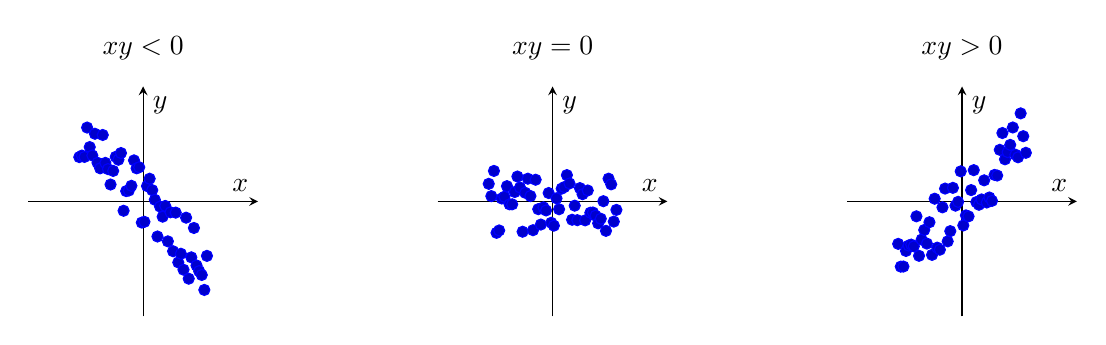
\begin{tikzpicture}
		 % Negative covariance
		\begin{scope}[shift={(0,0)}]
			\begin{axis}[
				width=4.5cm, height=4.5cm,
						 title={$\cov{x}{y} <0$},
				xlabel={$x$}, ylabel={$y$},
				xmin=-3, xmax=3, ymin=-3, ymax=3,
				xtick=\empty, ytick=\empty,
				axis lines=middle, enlargelimits
				]
				\addplot+[only marks, mark=*, samples=50, domain=-2:2] 
				({x}, {-x + rand});
			\end{axis}
		\end{scope}
		% Zero covariance
		\begin{scope}[shift={(5.2cm,0)}]
			\begin{axis}[
				width=4.5cm, height=4.5cm,
				 title={$\cov{x}{y} =0$}, xlabel={$x$}, ylabel={$y$},
				xmin=-3, xmax=3, ymin=-3, ymax=3,
				xtick=\empty, ytick=\empty,
				axis lines=middle, enlargelimits
				]
				\addplot+[only marks, mark=*, samples=50, domain=-2:2] 
				({x}, {rand});
			\end{axis}
		\end{scope}
		% Positive covariance
		\begin{scope}[shift={(10.4cm,0)}]
			\begin{axis}[
				width=4.5cm, height=4.5cm,
				 title={$\cov{x}{y} > 0$},
				xlabel={$x$}, ylabel={$y$},
				xmin=-3, xmax=3, ymin=-3, ymax=3,
				xtick=\empty, ytick=\empty,
				axis lines=middle, enlargelimits
				]
				\addplot+[only marks, mark=*, samples=50, domain=-2:2] 
				({x}, {x + rand});
			\end{axis}
		\end{scope}
		\end{tikzpicture}
			\caption{\Glspl{scatterplot} che mostrano \glspl{realization} ottenute da tre diversi \glspl{probmodel} per due 
				\glspl{rv} con diversi valori di covarianza: negativa (a sinistra), nulla (al centro) e positiva (a destra).}
			\label{fig:covariance-examples_dict}
		\end{figure}
		},
	first={covarianza},
	text={covarianza} 
}

\newglossaryentry{gmm}{name={Gaussian mixture model (GMM)}, description={A GMM\index{Gaussian mixture model (GMM)} 
		is a particular type of \gls{probmodel} for a numeric vector $\featurevec$ (e.g., 
		the \gls{feature}s of a \gls{datapoint}). Within a GMM, the vector $\featurevec$ is drawn from a randomly 
		selected \gls{mvndist} $p^{(\clusteridx)} = \mvnormal{\meanvec{\clusteridx}}{\covmtx{\clusteridx}}$ with 
		$\clusteridx = I$. The index $I \in \{1,\ldots,\nrcluster\}$ is an \gls{rv} with probabilities $\prob{I=\clusteridx} = p_{\clusteridx}$.
	     Note that a GMM is parametrized by the probability $p_{\clusteridx}$, the 
		\gls{mean} vector $\clustermean{\clusteridx}$, and the \gls{covmtx} $\bf\Sigma^{(\clusteridx)}$ for each $\clusteridx=1,\ldots,\nrcluster$. 
		GMMs are widely used for \gls{clustering}, density estimation, and as a generative \gls{model}. 
	 },first={Gaussian mixture model (GMM)},text={GMM} }
 
\newglossaryentry{maxlikelihood}{name={maximum likelihood}, description={
		Consider\index{maximum likelihood} \gls{datapoint}s $\dataset=\big\{ \datapoint^{(1)}, \ldots, \datapoint^{(\samplesize)} \}$ 
		that are interpreted as the \gls{realization}s of \gls{iid} \gls{rv}s with a common \gls{probdist} $\prob{\datapoint; \weights}$ which 
		depends on the \gls{modelparams} $\weights \in \mathcal{W} \subseteq \mathbb{R}^{n}$. 
		\Gls{maximum} likelihood methods learn \gls{modelparams} $\weights$ by maximizing 
		the probability (density) $\prob{\dataset; \weights} = \prod_{\sampleidx=1}^{\samplesize} \prob{\datapoint^{(\sampleidx)}; \weights}$ 
		of the observed \gls{dataset}. Thus, the \gls{maximum} likelihood estimator is a 
		solution to the optimization problem $\max_{\weights \in \mathcal{W}} \prob{\dataset; \weights}$.
	},first={maximum likelihood},text={maximum likelihood}}



\newglossaryentry{em}{name={expectation-maximization (EM)}, description={
		\index{expectation-maximization (EM)} 
		Consider a \gls{probmodel} $\prob{\datapoint; \weights}$ for the \gls{datapoint}s $\dataset$ generated in some 
		\gls{ml} application. The \gls{maxlikelihood} estimator for the \gls{modelparams} $\weights$ is obtained by maximizing 
		$\prob{\dataset; \weights}$. However, the resulting optimization problem might be computationally 
		challenging. \Gls{expectation}-maximization approximates the \gls{maxlikelihood} estimator by introducing a latent 
		\gls{rv} $\vz$ such that maximizing $\prob{\dataset,\vz; \weights}$ would be easier \cite{BishopBook,hastie01statisticallearning,GraphModExpFamVarInfWainJor}. Since we 
		do not observe $\vz$, we need to estimate it from the observed \gls{dataset} $\dataset$ 
		using a conditional \gls{expectation}. The resulting estimate $\widehat{\vz}$ is then used to 
		compute a new estimate $\widehat{\weights}$ by solving $\max_{\weights} \prob{\dataset, \widehat{\vz}; \weights}$. 
		The crux is that the conditional \gls{expectation} $\widehat{\vz}$ depends on the \gls{modelparams} $\widehat{\weights}$, 
		which we have updated based on $\widehat{\vz}$. Thus, we have to re-calculate $\widehat{\vz}$, 
		which, in turn, results in a new choice $\widehat{\weights}$ for the \gls{modelparams}. In practice, 
		we repeat the computation of the conditional \gls{expectation} (i.e., the E-step) and the update 
		of the \gls{modelparams} (i.e., the M-step) until some \gls{stopcrit} is met. 
  },first={EM},text={EM}}

\newglossaryentry{ppca}{name={probabilistic principal component analysis (PPCA)}, description={Probabilistic\index{probabilistic principal component analysis (PPCA)} \gls{pca} 
		extends basic \gls{pca} by using a \gls{probmodel} for \gls{datapoint}s. The \gls{probmodel} of probabilistic \gls{pca} 
		reduces the task of dimensionality reduction to an estimation problem that can be solved using \gls{em} 
		methods.},first={probabilistic principal component analysis (PPCA)},text={PPCA}}
	
\newglossaryentry{polyreg}{name={polynomial regression}, description={Polynomial\index{polynomial regression} 
		\gls{regression} aims at learning a polynomial \gls{hypothesis} map to predict a numeric \gls{label} based
		 on the numeric \gls{feature}s of a \gls{datapoint}. For \gls{datapoint}s characterized by a single 
		 numeric \gls{feature}, polynomial \gls{regression} uses the \gls{hypospace} 
			$\hypospace^{(\rm poly)}_{\nrfeatures} \defeq \{ \hypothesis(x) = \sum_{\featureidx=0}^{\nrfeatures-1} x^{\featureidx} \weight_{\featureidx} \}.$
			The quality of a polynomial \gls{hypothesis} map is measured using the average \gls{sqerrloss} 
			incurred on a set of \gls{labeled datapoint}s (which we refer to as the 
			\gls{trainset}).},first={polynomial regression},text={polynomial regression}}

\newglossaryentry{linreg}{name={linear regression}, description={Linear\index{linear regression} 
		\gls{regression} aims to learn a linear \gls{hypothesis} map to predict a numeric \gls{label} based 
		on the numeric \gls{feature}s of a \gls{datapoint}. The quality of a linear \gls{hypothesis} map is 
		measured using the average \gls{sqerrloss} incurred on a set of \gls{labeled datapoint}s, 
		which we refer to as the \gls{trainset}.},first={linear regression},text={linear regression}}
        
\newglossaryentry{ridgeregression}{name={ridge regression}, description={Ridge\index{ridge regression} 
		\gls{regression} learns the \gls{weights} $\weights$ of a linear \gls{hypothesis} map $\hypothesis^{(\weights)}(\featurevec)= \weights^{T} \featurevec$. The quality of a particular choice for the \gls{modelparams} $\weights$ is measured by the sum 
		of two components. The first component is the average \gls{sqerrloss} incurred by $\hypothesis^{(\weights)}$ on a set of 
		\gls{labeled datapoint}s (i.e., the \gls{trainset}). The second component is the scaled squared 
		Euclidean \gls{norm} $\regparam \| \weights \|^{2}_{2}$ with a \gls{regularization} parameter 
		$\regparam > 0$. Adding $\regparam \| \weights \|^{2}_{2}$ to 
	    the average \gls{sqerrloss} is equivalent to replacing each original \gls{datapoint}s by the \gls{realization} 
	    of (infinitely many) \gls{iid} \gls{rv}s centered around these \gls{datapoint}s (see \gls{regularization}).},first={ridge regression},text={ridge regression}}


\newglossaryentry{expectation}
{name={valore atteso}, plural={valori attesi}, description={
		Si consideri\index{valore atteso} un \gls{featurevec} numeriche $\featurevec \in \mathbb{R}^{\featuredim}$ 
		che interpretiamo come una \gls{realization} di una \gls{rv} con una \gls{probdist} $p(\featurevec)$. 
		Il valore atteso di $\featurevec$ è definito come l'integrale $\expect \{ \featurevec \} \defeq \int \featurevec p(\featurevec)$. Si noti che
		il valore atteso è definito solo se tale integrale esiste, ovvero se la \gls{rv} è integrabile
		\cite{HalmosMeasure,BillingsleyProbMeasure,RudinBookPrinciplesMatheAnalysis}},first={valore atteso},text={valore atteso}}

\newglossaryentry{logreg}{name={logistic regression}, description={Logistic\index{logistic regression} \gls{regression} learns a 
		linear \gls{hypothesis} map (or \gls{classifier}) $\hypothesis(\featurevec) = \weights^{T} \featurevec$ 
		to predict a binary \gls{label} $\truelabel$ based on the numeric \gls{featurevec} $\featurevec$ of 
		a \gls{datapoint}. The quality of a linear \gls{hypothesis} map is measured by the average \gls{logloss} 
		on some \gls{labeled datapoint}s (i.e., the \gls{trainset}).},
		first={logistic regression},text={logistic regression}}
	
\newglossaryentry{logloss}{name={logistic loss}, description={Consider\index{logistic loss} 
		a \gls{datapoint} characterized by the \gls{feature}s $\featurevec$ and a binary \gls{label} $\truelabel \in \{-1,1\}$. 
		We use a real-valued \gls{hypothesis} $\hypothesis$ to predict the \gls{label} $\truelabel$ 
		from the \gls{feature}s $\featurevec$. The logistic \gls{loss} incurred by this \gls{prediction} is 
		defined as 
	\begin{equation} 
		\label{equ_log_loss_gls_dict}
		\lossfunc{(\featurevec,\truelabel)}{\hypothesis} \defeq  \log ( 1 + \exp(- \truelabel \hypothesis(\featurevec))).
\end{equation}
Carefully note that the expression \eqref{equ_log_loss_gls_dict} 
for the logistic \gls{loss} applies only for the \gls{labelspace} $\labelspace = \{ -1,1\}$ and when using 
the thresholding rule \eqref{equ_def_threshold_bin_classifier_dict}. },first={logistic loss},text={logistic loss}}
	
\newglossaryentry{hingeloss}{name={hinge loss}, description={Consider\index{hinge loss} a \gls{datapoint} 
		characterized by a \gls{featurevec} $\featurevec \in \mathbb{R}^{\featuredim}$ and a 
		binary \gls{label} $\truelabel \in \{-1,1\}$. The hinge \gls{loss} incurred by a real-valued 
		\gls{hypothesis} map $\hypothesis(\featurevec)$ is defined as 
		\begin{equation} 
			\label{equ_hinge_loss_gls_dict}
				\lossfunc{(\featurevec,\truelabel)}{\hypothesis} \defeq \max \{ 0 , 1 - \truelabel \hypothesis(\featurevec) \}. 
			\end{equation}
			\begin{center}
		%\begin{figure}[htbp]
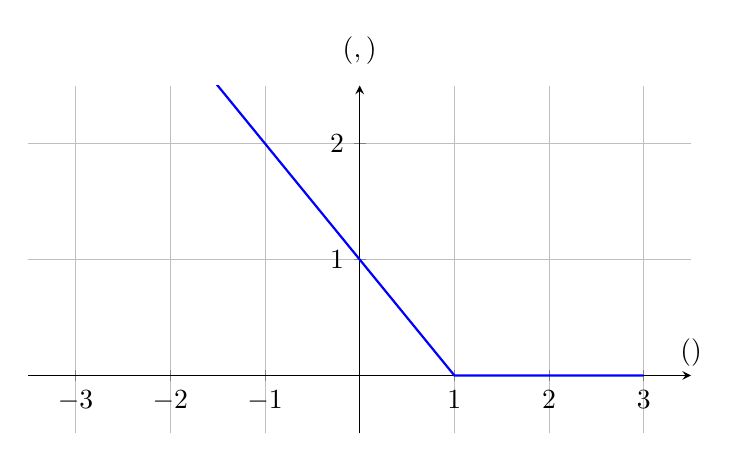
\begin{tikzpicture}
    \begin{axis}[
        axis lines=middle,
        xlabel={$\truelabel\hypothesis(\featurevec)$},
        ylabel={$\lossfunc{(\featurevec,\truelabel)}{\hypothesis}$},
 	xlabel style={at={(axis description cs:1.,0.3)}, anchor=north},  % Adjusted to be relative to axis end
        ylabel style={at={(axis description cs:0.5,1.1)}, anchor=center}, % Corrected to vertical position, rotated for readability
        xmin=-3.5, xmax=3.5,
        ymin=-0.5, ymax=2.5,
        xtick={-3, -2, -1, 0, 1, 2, 3},
        ytick={0, 1, 2},
        domain=-3:3,
        samples=100,
        width=10cm, height=6cm,
        grid=both,
        major grid style={line width=.2pt, draw=gray!50},
        minor grid style={line width=.1pt, draw=gray!20},
        legend pos=south west % Positions legend at the bottom left
    ]
        \addplot[blue, thick] {max(0, 1-x)};
     %   \addlegendentry{$\max(0, 1-x)$}
    \end{axis}
\end{tikzpicture}
	%	\end{figure} 
		\end{center}
	    A regularized variant of the hinge \gls{loss} is used by the \gls{svm} \cite{LampertNowKernel}. 	    
		},first={hinge loss},text={hinge loss}}

\newglossaryentry{iidasspt}
{name={independent and identically distributed assumption (i.i.d.\ assumption)}, 
	description={The \gls{iid} assumption\index{independent and identically distributed assumption (i.i.d.\ assumption)} interprets \glspl{datapoint} of a \gls{dataset} as the 
		\glspl{realization} of \gls{iid} \glspl{rv}.
				\\
		See also: \gls{iid}, \gls{datapoint}, \gls{dataset}, \gls{realization}, \gls{rv}.},
		first={independent and identically distributed assumption (i.i.d.\ assumption)},
		text={i.i.d.\ assumption} 
}

\newglossaryentry{hypospace}
{name={spazio delle ipotesi}, plural={spazi delle ipotesi}, description={Ogni\index{spazio delle ipotesi} 
		metodo pratico di \gls{ml} utilizza uno spazio delle \glspl{hypothesis} (o \gls{model}) $\hypospace$. Lo spazio delle
		 \glspl{hypothesis} di un metodo di \gls{ml} è un sottoinsieme di tutte le possibili \glspl{map} dallo \gls{featurespace} allo 
		 \gls{labelspace}. 
		La scelta nella definizione dello spazio delle \glspl{hypothesis} dovrebbe tenere in considerazione le risorse computazionali 
		disponibili e lo \gls{statasp}. Qualora l'infrastruttura computazionale consenta operazioni matriciali efficienti e sussista una 
		relazione (approssimativamente) lineare tra un insieme di \glspl{feature} e una \gls{label}, una scelta opportuna per lo 
		spazio delle \glspl{hypothesis} potrebbe essere il \gls{linmodel}.
				\\
		Si veda anche: \gls{ml}, \gls{hypothesis}, \gls{model}, \gls{map}, \gls{featurespace}, \gls{labelspace}, \gls{statasp}, \gls{feature}, \gls{label}, \gls{linmodel}.},first={spazio delle ipotesi},text={spazio delle ipotesi} }
	
\newglossaryentry{model}
{name={modello}, plural={modelli}, description={Nel\index{modello} contesto del \gls{ml}, 
		il termine modello si riferisce tipicamente allo \gls{hypospace} sottostante ad un metodo di
		\gls{ml} \cite{MLBasics}, \cite{ShalevMLBook}. Tuttavia, il termine è utilizzato anche in altri ambiti, ma con un significato 
		differente. Ad esempio, un \gls{probmodel} si riferisce a un insieme parametrizzato di \glspl{probdist}.
						\\
		Si veda anche: \gls{ml}, \gls{hypospace}, \gls{probmodel}, \gls{probdist}.},first={modello},text={modello} }

\newglossaryentry{modelparams}{name={model parameters}, 
	description={\Gls{model} \glspl{parameter}\index{model parameters} are quantities that 
	are used to select a specific \gls{hypothesis} \gls{map} from a \gls{model}. 
	We can think of a list of \gls{model} \glspl{parameter} as a unique identifier for a \gls{hypothesis} 
	\gls{map}, similar to how a social security number identifies a person in Finland.
			\\
		See also: \gls{model}, \gls{parameter}, \gls{hypothesis}, \gls{map}.},
	first={model parameters},
	text={model parameters} 
}
\newglossaryentry{ai}{name={artificial intelligence (AI)}, description={
		AI\index{artificial intelligence (AI)} refers to systems that behave rationally in the sense of 
		maximizing a long-term \gls{reward}. The \gls{ml}-based approach to AI is to train a \gls{model} for  
		predicting optimal actions. These predictions are computed from observations about the state of the 
		environment. The choice of \gls{lossfunc} sets AI applications apart from more basic \gls{ml} applications. 
		AI systems rarely have access to a labeled \gls{trainset} that allows the average \gls{loss} to be measured for any possible choice of \gls{modelparams}. 
		Instead, AI systems use observed \gls{reward} signals to obtain a (point-wise) estimate for the 
		\gls{loss} incurred by the current choice of \gls{modelparams}.},first={AI},text={AI} }

\newglossaryentry{reward}{name={reward}, description={A reward refers to some\index{reward} observed 
		(or measured) quantity that allows us to estimate the \gls{loss} incurred by the \gls{prediction} 
		(or decision) of a \gls{hypothesis} $\hypothesis(\featurevec)$. For example, in an 
		\gls{ml} application to self-driving vehicles, $\hypothesis(\featurevec)$ could represent 
		the current steering direction of a vehicle. We could construct a reward from the 
		measurements of a collision sensor that indicate if the vehicle is moving towards 
		an obstacle. We define a low reward for the steering direction 
	$\hypothesis(\featurevec)$ if the vehicle moves dangerously towards an obstacle.},
	first={reward}, text={reward}} 

\newglossaryentry{hardclustering}{name={hard clustering}, description={Hard \gls{clustering}\index{hard clustering} 
		refers to the task of partitioning a given set of \gls{datapoint}s into (a few) non-overlapping \gls{cluster}s. 
		The most widely used hard \gls{clustering} method is \gls{kmeans}.},first={hard clustering},text={hard clustering} }
	
\newglossaryentry{softclustering}{name={soft clustering}, description={Soft \gls{clustering}\index{soft clustering} 
		refers to the task of partitioning a given set of \gls{datapoint}s into (a few) overlapping \gls{cluster}s. 
		Each \gls{datapoint} is assigned to several different \gls{cluster}s with varying degrees of belonging. Soft \gls{clustering} 
		methods determine the \gls{dob} (or soft \gls{cluster} assignment) for each \gls{datapoint} and each \gls{cluster}.
		A principled approach to soft \gls{clustering} is by interpreting \gls{datapoint}s as \gls{iid} \gls{realization}s 
		of a \gls{gmm}. We then obtain a natural choice for the \gls{dob} as the conditional 
		\gls{probability} of a \gls{datapoint} belonging to a specific mixture component.},first={soft clustering},text={soft clustering} }
	
\newglossaryentry{clustering}{name={clustering}, description={Clustering\index{clustering} methods decompose a given 
		set of \gls{datapoint}s into a few subsets, which are referred to as \gls{cluster}s. 
		Each \gls{cluster} consists of \gls{datapoint}s that are more similar to each 
		other than to \gls{datapoint}s outside the \gls{cluster}. Different clustering methods 
		use different measures for the similarity between \gls{datapoint}s and different 
		forms of \gls{cluster} representations. The clustering method \gls{kmeans} uses the 
		average \gls{feature} vector (cluster \gls{mean}) of a \gls{cluster} as its representative. 
		A popular \gls{softclustering} method based on \gls{gmm} represents 
		a \gls{cluster} by a \gls{mvndist}.},first={clustering},text={clustering} }
	
\newglossaryentry{cluster}{name={cluster}, 
	description={A\index{cluster} cluster is a subset of 
		\glspl{datapoint} that are more similar to each other than to the \glspl{datapoint} outside the cluster. 
		The quantitative measure of similarity between \glspl{datapoint} is a design choice. If \glspl{datapoint} 
		are characterized by Euclidean \glspl{featurevec} $\featurevec \in \mathbb{R}^{\nrfeatures}$, 
		we can define the similarity between two \glspl{datapoint} via the Euclidean distance between 
		their \glspl{featurevec}. An example of such clusters is shown in Fig.~\ref{fig:clusters}.\\
		\begin{figure}[H]
		\centering
		\begin{tikzpicture}
		\pgfplotsset{compat=1.18}
		\begin{axis}[
		    width=10cm,
		    height=8cm,
		    xlabel={$x_1$},
		    ylabel={$x_2$},
		    title={Clusters of Data Points},
		    xmin=0, xmax=10,
		    ymin=0, ymax=10,
		    axis lines=left,
		    legend style={at={(0.5,-0.25)}, anchor=north, legend columns=3}
		]
		% Cluster 1 
		\addplot[only marks, color=blue, mark=*, mark size=3pt] coordinates {
		    (1,1) (2,1.2) (1.8,2) (2.2,1.5) (1.5,2.5)
		};
		% Cluster 2 
		\addplot[only marks, color=red, mark=square*, mark size=3pt] coordinates {
		    (7,8) (8,7.5) (7.5,8.5) (8.2,7.8) (7.7,7)
		};
		% Cluster 3 
		\addplot[only marks, color=green!60!black, mark=triangle*, mark size=3pt] coordinates {
		    (5,3) (5.5,3.2) (5.2,2.8) (4.8,3.5) (5.1,3.1)
		};
		\legend{Cluster 1, Cluster 2, Cluster 3}
		\end{axis}
		\end{tikzpicture}
		\caption{Illustration of three clusters in a two-dimensional \gls{featurespace}. Each cluster groups \glspl{datapoint} that are more similar to each other than to those in other clusters, based on the Euclidean distance.}
		\label{fig:clusters}
		\end{figure}
		See also: \gls{datapoint}, \gls{featurevec}, \gls{featurespace}.
		},
		first={cluster},text={cluster} }

%\newglossaryentry{softclustering}{name={soft clustering}, description={Soft clustering methods determine, for each \gls{datapoint} within a dataset, 
%		a soft cluster assignment or the degree of belonging to a particular cluster.},first={soft clustering},text={soft clustering} }


\newglossaryentry{huberloss}{name={Huber loss}, description={The\index{Huber loss} 
		Huber \gls{loss} unifies the \gls{sqerrloss} and the \gls{abserr}.},first={Huber loss},text={Huber loss} }

\newglossaryentry{svm}{name={support vector machine (SVM)}, description={The\index{support vector machine (SVM)} 
		SVM is a binary \gls{classification} method that 
		learns a linear \gls{hypothesis} map. Thus, like \gls{linreg} and \gls{logreg}, 
		it is also an instance of \gls{erm} for the \gls{linmodel}. However, the 
		SVM uses a different \gls{lossfunc} from the one used in those methods. As illustrated in 
		Figure \ref{fig_svm_gls_dict}, it aims to maximally separate \gls{datapoint}s from 
		the two different classes in the \gls{featurespace} (i.e., \gls{maximum} margin principle). 
		Maximizing this separation is equivalent to minimizing a regularized 
		variant of the \gls{hingeloss} \eqref{equ_hinge_loss_gls_dict} \cite{LampertNowKernel,Cristianini_Shawe-Taylor_2000,BishopBook}.
		\begin{figure}[H]
			\begin{center}
				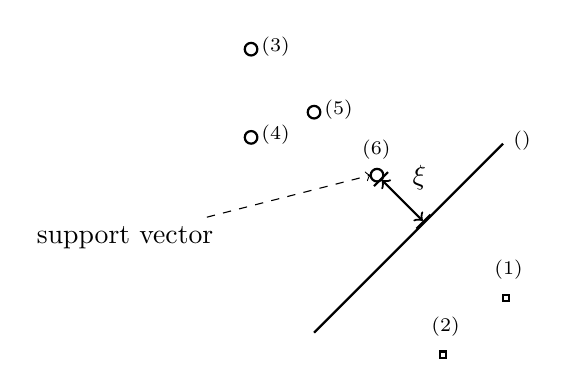
\begin{tikzpicture}[auto,scale=0.8]
					%\draw [thick] (0,-3) rectangle (4,4) node [anchor=east,above] {$\featurespace$} ;
					\draw [thick] (1,2) circle (0.1cm)node[anchor=west] {\hspace*{0mm}$\featurevec^{(5)}$};
					\draw [thick] (0,1.6) circle (0.1cm)node[anchor=west] {\hspace*{0mm}$\featurevec^{(4)}$};
					\draw [thick] (0,3) circle (0.1cm)node[anchor=west] {\hspace*{0mm}$\featurevec^{(3)}$};
					\draw [thick] (2,1) circle (0.1cm)node[anchor=east,above] {\hspace*{0mm}$\featurevec^{(6)}$};
					\node[] (B) at (-2,0) {support vector};
					\draw[->,dashed] (B) to (1.9,1) ; 
					\draw [|<->|,thick] (2.05,0.95)  -- (2.75,0.25)node[pos=0.5] {$\xi$} ; 
					\draw [thick] (1,-1.5) -- (4,1.5) node [right] {$\hypothesis^{(\weights)}$} ; 
					\draw [thick] (3,-1.9) rectangle ++(0.1cm,0.1cm) node[anchor=west,above]  {\hspace*{0mm}$\featurevec^{(2)}$};
					\draw [thick] (4,.-1) rectangle ++(0.1cm,0.1cm) node[anchor=west,above] {\hspace*{0mm}$\featurevec^{(1)}$};
				\end{tikzpicture}
				\caption{The \gls{svm} learns a \gls{hypothesis} (or \gls{classifier}) $\hypothesis^{(\weights)}$ with 
					minimal average soft-margin \gls{hingeloss}. Minimizing this \gls{loss} is equivalent 
					to maximizing the margin $\xi$ between the \gls{decisionboundary} of $\hypothesis^{(\weights)}$ 
					and each class of the \gls{trainset}.}
				\label{fig_svm_gls_dict}
			\end{center}
		\end{figure}
		The above basic variant of SVM is only useful if the \gls{datapoint}s from different categories can be  
		(approximately) linearly separated. For an \gls{ml} application where the categories are not 
		%linearly separable based on the the original (raw) \gls{feature}s it is possible to apply the SVM 
		%to transformed \gls{feature}s. These transformed \gls{feature}s can be obtained by applying a \gls{featuremap} 
		derived from a \gls{kernel}.
},first={support vector machine (SVM)},text={SVM} }

\newglossaryentry{eigenvalue}{name={eigenvalue}, description={We\index{eigenvalue} refer to a 
		number $\lambda \in \mathbb{R}$ as an eigenvalue of a square matrix $\mathbf{A} \in \mathbb{R}^{\featuredim \times \featuredim}$ 
		if there is a non-zero vector $\vx \in \mathbb{R}^{\featuredim} \setminus \{ \mathbf{0} \}$ such that $\mathbf{A} \vx = \lambda \vx$. },first={eigenvalue},text={eigenvalue} }
	
\newglossaryentry{eigenvector}{name={eigenvector}, description={An\index{eigenvector} 
		eigenvector of a matrix $\mathbf{A} \in \mathbb{R}^{\featuredim \times \featuredim}$ 
		is a non-zero vector $\vx \in \mathbb{R}^{\featuredim} \setminus \{ \mathbf{0} \}$ 
		such that $\mathbf{A} \vx = \lambda \vx$ with some \gls{eigenvalue} $\lambda$.},first={eigenvector},text={eigenvector} }

\newglossaryentry{evd}{name={eigenvalue decomposition (EVD)}, 
	description={The\index{eigenvalue decomposition (EVD)} \gls{eigenvalue} 
		decomposition for a square matrix $\mA \in \mathbb{R}^{\dimlocalmodel \times \dimlocalmodel}$ 
		is a factorization of the form 
		$$\mA = \mathbf{V} {\bm \Lambda} \mathbf{V}^{-1}.$$ 
		The columns of the matrix $\mV = \big( \vv^{(1)},\ldots,\vv^{(\dimlocalmodel)} \big)$ are the 
		\gls{eigenvector}s of the matrix $\mV$. The diagonal matrix 
		${\bm \Lambda} = {\rm diag} \big\{ \eigval{1},\ldots,\eigval{\dimlocalmodel} \big\}$ 
		contains the \gls{eigenvalue}s $\eigval{\featureidx}$ corresponding to the \gls{eigenvector}s $\vv^{(\featureidx)}$. 
		Note that the above decomposition exists only if the matrix $\mA$ is diagonalizable.},first={eigenvalue decomposition (EVD)},text={EVD} }

\newglossaryentry{svd}{name={singular value decomposition (SVD)}, 
  	description={The\index{singular value decomposition (SVD)} SVD  
  		for a matrix $\mA \in \mathbb{R}^{\samplesize \times \dimlocalmodel}$ 
		is a factorization of the form 
		$$\mA = \mathbf{V} {\bm \Lambda} \mathbf{U}^{T},$$ 
		with orthonormal matrices $\mV \in \mathbb{R}^{\samplesize \times \samplesize}$ 
		and $\mU \in \mathbb{R}^{\dimlocalmodel \times \dimlocalmodel}$ \cite{GolubVanLoanBook}. 
		The matrix ${\bm \Lambda} \in \mathbb{R}^{\samplesize \times \dimlocalmodel}$ is 
		only non-zero along the main diagonal, whose entries $\Lambda_{\featureidx,\featureidx}$ 
		are non-negative and referred to as singular values.
	},first={singular value decomposition (SVD)},text={SVD} }


\newglossaryentry{tv}{name={total variation}, description={See \gls{gtv}\index{total variation}.},
	first={total variation},text={total variation} }

 \newglossaryentry{cvxclustering}{name={convex clustering}, 
 	description={Consider\index{convex clustering} a \gls{dataset} 
 	$\featurevec^{(1)},\ldots,\featurevec^{(\samplesize)} \in \mathbb{R}^{\nrfeatures}$. 
 	\Gls{convex} \gls{clustering} learns vectors $\weights^{(1)},\ldots,\weights^{(\samplesize)}$ by 
 	minimizing 
 	$$ \sum_{\sampleidx=1}^{\samplesize} \normgeneric{\featurevec^{(\sampleidx)} - \weights^{(\sampleidx)}}{2}^2 + 
 	\regparam \sum_{\nodeidx,\nodeidx' \in \nodes} \normgeneric{\weights^{(\nodeidx)} - \weights^{(\nodeidx')}}{p}.$$ 
	Here, $ \normgeneric{\vu}{p} \defeq \big( \sum_{\featureidx=1}^{\dimlocalmodel} |u_{\featureidx}|^{p} \big)^{1/p}$ 
	denotes the $p$-\gls{norm} (for $p\geq1$).  
	It turns out that many of the optimal vectors $\widehat{\weights}^{(1)},\ldots,\widehat{\weights}^{(\samplesize)}$ 
	coincide. A \gls{cluster} then consists of those \gls{datapoint}s $\sampleidx \in \{1,\ldots,\samplesize\}$ 
	with identical $\widehat{\weights}^{(\sampleidx)}$ \cite{JMLR:v22:18-694,Pelckmans2005}. 
 	  },
 		first={convex clustering},text={convex clustering} }


\newglossaryentry{gdmethods}{name={gradient-based methods}, 
	description={\Gls{gradient}-based\index{gradient-based methods} 
		methods are iterative techniques for finding the \gls{minimum} (or \gls{maximum}) 
		of a \gls{differentiable} \gls{objfunc} of the \gls{modelparams}. These 
		methods construct a sequence of approximations to an optimal choice for 
		\gls{modelparams} that results in a \gls{minimum} (or \gls{maximum}) value of the \gls{objfunc}. 
		As their name indicates, \gls{gradient}-based methods use the \gls{gradient}s of the \gls{objfunc} 
		evaluated during previous iterations to construct new, (hopefully) improved \gls{modelparams}. 
		One important example of a \gls{gradient}-based method is \gls{gd}.},
		first={gradient-based methods},text={gradient-based methods} }

\newglossaryentry{sgd}{name={subgradient descent}, description={\Gls{subgradient}\index{subgradient descent} 
		descent is a \gls{generalization} of \gls{gd} that does not require differentiability of the 
		function to be minimized. This \gls{generalization} is obtained by replacing the concept 
		of a \gls{gradient} with that of a \gls{subgradient}. Similar to \gls{gradient}s, also \gls{subgradient}s 
		allow us to construct local approximations of an \gls{objfunc}. The \gls{objfunc} 
		might be the \gls{emprisk} $\emperror\big( \hypothesis^{(\weights)} \big| \dataset \big)$ viewed 
		as a function of the \gls{modelparams} $\weights$ that select a \gls{hypothesis} $\hypothesis^{(\weights)} \in \hypospace$.},first={subgradient descent},text={subgradient descent} }
	
\newglossaryentry{stochGD}{name={stochastic gradient descent (SGD)}, description={Stochastic\index{stochastic gradient descent (SGD)} 
		\gls{gd} is obtained from \gls{gd} by replacing the \gls{gradient} of the \gls{objfunc} 
		with a stochastic approximation. A main application of stochastic \gls{gd} 
		is to train a parametrized \gls{model} via \gls{erm} on a \gls{trainset} $\dataset$ that 
		is either very large or not readily available (e.g., when \gls{datapoint}s are stored 
		in a database distributed all over the planet). To evaluate the \gls{gradient} of the 
		\gls{emprisk} (as a function of the \gls{modelparams} $\weights$), 
		we need to compute a sum $\sum_{\sampleidx=1}^{\samplesize} \nabla_{\weights} \lossfunc{\datapoint^{(\sampleidx)}}{\weights}$  
		over all \gls{datapoint}s in the \gls{trainset}. We obtain a stochastic 
		approximation to the \gls{gradient} by replacing the sum $\sum_{\sampleidx=1}^{\samplesize} \nabla_{\weights} \lossfunc{\datapoint^{(\sampleidx)}}{\weights}$ 
		with a sum $\sum_{\sampleidx \in \batch} \nabla_{\weights} \lossfunc{\datapoint^{(\sampleidx)}}{\weights}$ 
		over a randomly chosen subset $\batch \subseteq \{1,\ldots,\samplesize\}$ (see Figure \ref{fig_sgd_approx_dict}). 
		We often refer to these randomly chosen \gls{datapoint}s as a \gls{batch}. 
		The \gls{batch} size $|\batch|$ is an important parameter of stochastic \gls{gd}. 
		Stochastic \gls{gd} with $|\batch|> 1$ is referred to as mini-\gls{batch} stochastic \gls{gd} \cite{Bottou99}. 		
		\begin{figure}[H]
			\centering
			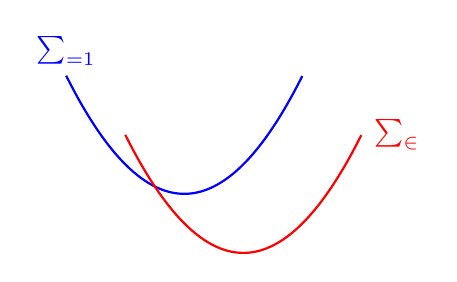
\begin{tikzpicture}[scale=1.5, >=stealth]
% Axes
				%\draw[->] (-1, 0) -- (4, 0) node[right] {$w$};
				%\draw[->] (0, -0.5) -- (0, 4) node[above] {};
% First quadratic function: f(w)
				\draw[thick, blue, domain=0.5:2.5, samples=100] plot (\x, {(\x-1.5)^2 + 1});
				\node[blue,above] at (0.5, 2) {$\sum_{\sampleidx=1}^{\samplesize}$};
% Second quadratic function: f'(w)
				\draw[thick, red, domain=1:3, samples=100] plot (\x, {(\x-2)^2 + 0.5});
				\node[red] at (3.3, 1.5) {$\sum_{\sampleidx \in \batch}$};
% Labels
			\end{tikzpicture}
		\caption{Stochastic \gls{gd} for \gls{erm} approximates the \gls{gradient} 
		$\sum_{\sampleidx=1}^{\samplesize} \nabla_{\weights} \lossfunc{\datapoint^{(\sampleidx)}}{\weights}$ 
		by replacing the 
		sum over all \gls{datapoint}s in the \gls{trainset} (indexed by $\sampleidx=1,\ldots,\samplesize$) 
		with a sum over a randomly chosen subset $\batch \subseteq \{1,\ldots,\samplesize\}$.\label{fig_sgd_approx_dict}}
		\end{figure}
},first={stochastic gradient descent (SGD)},text={SGD} }


\newglossaryentry{onlineGD}{name={online gradient descent (online GD)}, description={
Consider \index{online gradient descent (online GD)} an \gls{ml} method that learns \gls{modelparams} 
$\weights$ from some \gls{paramspace} $\paramspace \subseteq \mathbb{R}^{\dimlocalmodel}$. 
The learning process uses \gls{datapoint}s $\datapoint^{(\timeidx)}$ that arrive at consecutive time-instants $\timeidx=1,2,\ldots$. 
Let us interpret the \gls{datapoint}s $\datapoint^{(\timeidx)}$ as \gls{iid} copies 
of an \gls{rv} $\datapoint$. The \gls{risk} $\expect\{ \lossfunc{\datapoint}{\weights} \}$ of a 
\gls{hypothesis} $\hypothesis^{(\weights)}$ can then (under mild conditions) be obtained as the limit 
$\lim_{T\rightarrow \infty} (1/T)\sum_{\timeidx=1}^{T} \lossfunc{\datapoint^{(\timeidx)}}{\weights}$. 
We might use this limit as the \gls{objfunc} for learning the \gls{modelparams} $\weights$. 
Unfortunately, this limit can only be evaluated if we wait infinitely long in order to collect all \gls{datapoint}s. 
Some \gls{ml} applications require methods that learn online: as soon as a new \gls{datapoint} $\datapoint^{(\timeidx)}$ 
arrives at time $\timeidx$, we update the current \gls{modelparams} $\weights^{(\timeidx)}$. Note that 
the new \gls{datapoint} $\datapoint^{(\timeidx)}$ contributes the component $\lossfunc{\datapoint^{(\timeidx)}}{\weights}$ 
to the \gls{risk}. As its name suggests, online \gls{gd} updates $\weights^{(\timeidx)}$ via a (projected) \gls{gradstep}
\begin{equation} 
\label{equ_def_ogd_dict}
 \weights^{(\timeidx+1)} \defeq \projection{\paramspace}{\weights^{(\timeidx)} - \lrate_{\timeidx} \nabla_{\weights} \lossfunc{\datapoint^{(\timeidx)}}{\weights}}. 
\end{equation} 
Note that \eqref{equ_def_ogd_dict} is a \gls{gradstep} for the current component $\lossfunc{\datapoint^{(\timeidx)}}{\cdot}$ 
of the \gls{risk}. The update \eqref{equ_def_ogd_dict} ignores all the previous components $\lossfunc{\datapoint^{(\timeidx')}}{\cdot}$, 
for $\timeidx' < \timeidx$. It might therefore happen that, compared to $\weights^{(\timeidx)}$, the updated \gls{modelparams} 
$\weights^{(\timeidx+1)}$ increase the retrospective average \gls{loss} $\sum_{\timeidx'=1}^{\timeidx-1} \lossfunc{\datapoint^{(\timeidx')}}{\cdot}$. 
However, for a suitably chosen \gls{learnrate} $\lrate_{\timeidx}$, online \gls{gd} can be shown 
to be optimal in practically relevant settings. By optimal, we mean that the \gls{modelparams} 
$\weights^{(T+1)}$ delivered by online \gls{gd} after observing $T$ \gls{datapoint}s $\datapoint^{(1)},\ldots, \datapoint^{(T)}$ 
are at least as good as those delivered by any other learning method \cite{HazanOCO,GDOptimalRakhlin2012}. 
\begin{figure}[H]
	\begin{center}
\begin{tikzpicture}[x=1.5cm,scale=1.5, every node/.style={font=\footnotesize}]
	% Axes
	\draw[->] (0.5, 0) -- (5.5, 0) node[below] {};
	%\draw[->] (0, -0.5) -- (0, 3) node[left] {Value};
	% Labels for time steps
	\foreach \x in {1, 2, 3, 4, 5} {
		\draw (\x, 0.1) -- (\x, -0.1) node[below] {$t=\x$};
	}
	% Data points (black circles)
	\foreach \x/\y in {1/2.5, 2/1.8, 3/2.3, 4/1.5, 5/2.0} {
		\fill[black] (\x, \y) circle (2pt) node[above right] {$\datapoint^{(\x)}$};
	}
	% Model parameters (blue circles)
	\foreach \x/\y in {1/1.0, 2/1.6, 3/1.8, 4/2.2, 5/1.9} {
		\fill[blue] (\x, \y) circle (2pt) node[below left] {$\weights^{(\x)}$};
	}
	% Connecting lines (model tracking data)
	\foreach \x/\y/\z in {1/2.5/1.0, 2/1.8/1.6, 3/2.3/2.0, 4/1.5/1.8, 5/2.0/1.9} {
		\draw[dashed, gray] (\x, \y) -- (\x, \z);
	}
	% Legend
	% \node[draw, fill=white] at (4.5, 2.7) {
	% 	\begin{tabular}{@{}ll@{}}
	% 		\textcolor{black}{$\bullet$} & Data Point ($d_t$) \\
	% 		\textcolor{blue}{$\bullet$} & Model Parameter ($\theta_t$) \\
	% 		\textcolor{gray}{\rule{1cm}{0.5pt}} & Gradient Update
	% 	\end{tabular}
	%};
	\end{tikzpicture}
\end{center} 
\caption{An instance of online \gls{gd} that updates the \gls{modelparams} $\weights^{(\timeidx)}$ 
using the \gls{datapoint} $\datapoint^{(\timeidx)} = \feature^{(\timeidx)}$ arriving at time $\timeidx$. 
This instance uses the \gls{sqerrloss} $\lossfunc{\datapoint^{(\timeidx)}}{\weight} = (\feature^{(\timeidx)} - \weight)^{2}$.
}
\end{figure}},
first={online gradient descent (online GD)},text={online GD}}

\newglossaryentry{pca}{name={principal component analysis (PCA)}, description={PCA\index{principal component analysis (PCA)} 
		determines a linear \gls{featuremap} such that the new \gls{feature}s 
		allow us to reconstruct the original \gls{feature}s with the \gls{minimum} reconstruction error \cite{MLBasics}.},first={principal component analysis (PCA)},text={PCA} }
	
\newglossaryentry{loss}
{name={perdita}, 
	description={\I metodi di gls{ml}\index{perdita} utilizzano una 
		\gls{lossfunc} $\lossfunc{\datapoint}{\hypothesis}$ per misurare l’errore commesso 
		applicando una specifica \gls{hypothesis} ad un determinato \gls{datapoint}. Con un lieve 
		abuso di notazione, utilizziamo il termine perdita sia per indicare la \gls{lossfunc} $\loss$ 
		in sé, sia per il valore specifico $\lossfunc{\datapoint}{\hypothesis}$, relativo a un \gls{datapoint} $\datapoint$ 
		e ad una \gls{hypothesis} $\hypothesis$.
				\\
		Si ved anche: \gls{ml}, \gls{lossfunc}, \gls{hypothesis}, \gls{datapoint}.},first={perdita},text={perdita} }

\newglossaryentry{lossfunc}{name={loss function}, description={A\index{loss function} \gls{loss} function is a map 
		$$\lossfun: \featurespace \times \labelspace \times \hypospace \rightarrow \mathbb{R}_{+}: \big( \big(\featurevec,\truelabel\big),
		 \hypothesis\big) \mapsto  \lossfunc{(\featurevec,\truelabel)}{\hypothesis}.$$
		It assigns a non-negative real number (i.e., the \gls{loss}) $\lossfunc{(\featurevec,\truelabel)}{\hypothesis}$
		to a pair that consists of a \gls{datapoint}, with \gls{feature}s $\featurevec$ 
		and \gls{label} $\truelabel$, and a \gls{hypothesis} $\hypothesis \in \hypospace$. The 
		value $\lossfunc{(\featurevec,\truelabel)}{\hypothesis}$ quantifies the discrepancy 
		between the true \gls{label} $\truelabel$ and the \gls{prediction} $\hypothesis(\featurevec)$. 
		Lower (closer to zero) values $\lossfunc{(\featurevec,\truelabel)}{\hypothesis}$ indicate a smaller 
		discrepancy between \gls{prediction} $\hypothesis(\featurevec)$ and \gls{label} $\truelabel$. 
		Figure \ref{fig_loss_function_gls_dict} depicts a \gls{loss} function for a given \gls{datapoint}, 
		with \gls{feature}s $\featurevec$ and \gls{label} $\truelabel$, as a function of the \gls{hypothesis} $\hypothesis \in \hypospace$. 
		\begin{figure}[H]
			\begin{center}
				\begin{tikzpicture}[scale = 0.7]
					\begin{axis}
						[%grid, 
						axis x line=center,
						axis y line=center,
						%	xtick={-2,-1,...,2},
						%	ytick={0,1,...,2},
						xlabel={},
						%	ylabel={\hspace*{3mm} loss $\lossfun$},
						xlabel style={below right},
						ylabel style={above right},
						xtick=\empty,
						ytick=\empty,
						xmin=-4,
						xscale = 1.4, 
						xmax=4,
						ymin=-0.5,
						ymax=2.5
						]
						\addplot [smooth, ultra thick] table [x=a, y=b, col sep=comma] {assets/logloss.csv};    
					\end{axis}
					\node [above] at (1,5) {$\lossfunc{(\featurevec,\truelabel)}{\hypothesis}$};
					\node [above] at (10,1) {\gls{hypothesis} $\hypothesis$};
						\node [right] at (4,6) {\gls{loss}};
				\end{tikzpicture}
			\end{center}
			\vspace*{-7mm}
			\caption{Some \gls{loss} function $\lossfunc{(\featurevec,\truelabel)}{\hypothesis}$ for a fixed \gls{datapoint}, with 
				\gls{featurevec} $\featurevec$ and \gls{label} $\truelabel$, and a varying \gls{hypothesis} $\hypothesis$. 
				\gls{ml} methods try to find (or learn) a \gls{hypothesis} that incurs minimal \gls{loss}.}
			\label{fig_loss_function_gls_dict}
	\end{figure}
 },first={loss function},text={loss function} }

\newglossaryentry{decisiontree}{name={decision tree}, description={A\index{decision tree} 
		decision tree is a flow-chart-like representation of a \gls{hypothesis} map $\hypothesis$. 
		More formally, a decision tree is a directed \gls{graph} containing a root node that reads 
		in the \gls{featurevec} $\featurevec$ of a \gls{datapoint}. The root node then forwards 
		the \gls{datapoint} to one of its children nodes based on some elementary test on the \gls{feature}s $\featurevec$. 
		If the receiving child node is not a leaf node, i.e., it has itself children nodes, 
	  it represents another test. Based on the test result, the \gls{datapoint} is forwarded 
	   to one of its descendants. This testing and forwarding of the \gls{datapoint} is continued 
	  until the \gls{datapoint} ends up in a leaf node (having no children nodes). 
\begin{figure}[H]
\begin{minipage}{.45\textwidth}
	\scalebox{1}{
\begin{tikzpicture}
%	% Root node
	\node[fill=black, circle, inner sep=2pt, label=above:{$\| \featurevec-\mathbf{u} \| \leq \varepsilon$?}] (A) {};	
%	% Left child (h1)
	\node[fill=black, circle, inner sep=2pt, below left=1.5cm and 1cm of A, label=left:{$\hypothesis(\featurevec) = \predictedlabel_1$}] (B) {};
	% Right child (next question)
	\node[fill=black, circle, inner sep=2pt, below right=1.5cm and 1cm of A, label=right:{$\| \featurevec - \mathbf{v} \| \leq \varepsilon$?}] (C) {};
%	% Left child of C (h2)
	\node[fill=black, circle, inner sep=2pt, below left=1.5cm and 1cm of C, label=left:{$\hypothesis(\featurevec) = \predictedlabel_2$}] (D) {};
	% Right child of C (h3)
	\node[fill=black, circle, inner sep=2pt, below right=1.5cm and 1cm of C, label=right:{$\hypothesis(\featurevec) =\predictedlabel_3$}] (E) {};
%	% Arrows
	\draw[line width=1.5pt, ->] (A) -- (B) node[midway, left] {no};
	\draw[line width=1.5pt, ->] (A) -- (C) node[midway, right] {yes};
	\draw[line width=1.5pt, ->] (C) -- (D) node[midway, left] {no};
	\draw[line width=1.5pt, ->] (C) -- (E) node[midway, right] {yes};
\end{tikzpicture}
	}
\end{minipage}	
\hspace*{15mm}
\begin{minipage}{.45\textwidth}
	\hspace*{15mm}
	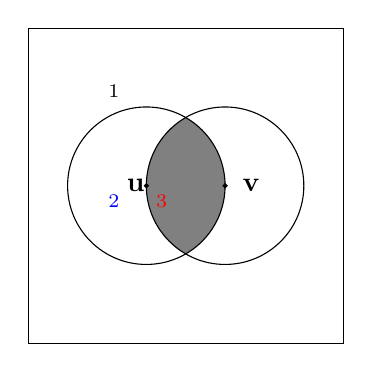
\begin{tikzpicture}
		\draw (-2,2) rectangle (2,-2);
		\begin{scope}
			\clip (-0.5,0) circle (1cm);
			\clip (0.5,0) circle (1cm);
			\fill[color=gray] (-2,1.5) rectangle (2,-1.5);
		\end{scope}
		\draw (-0.5,0) circle (1cm);
		\draw (0.5,0) circle (1cm);
		\draw[fill] (-0.5,0) circle [radius=0.025];
		\node [below right, red] at (-0.5,0) {$\predictedlabel_{3}$};
		\node [below left, blue] at (-0.7,0) {$\predictedlabel_{2}$};
		\node [above left] at (-0.7,1) {$\predictedlabel_{1}$};
		\node [left] at (-0.4,0) {$\mathbf{u}$};
		\draw[fill] (0.5,0) circle [radius=0.025];
		\node [right] at (0.6,0) {$\mathbf{v}$};
	\end{tikzpicture}
\end{minipage}
	\caption{Left: A decision tree is a flow-chart-like representation of a piece-wise constant \gls{hypothesis} $\hypothesis: \featurespace \rightarrow \mathbb{R}$.  Each piece is a \gls{decisionregion} $\decreg{\predictedlabel} \defeq \big\{ \featurevec \in  \featurespace: \hypothesis(\featurevec) = \predictedlabel \big\}$. 
		The depicted decision tree can be applied to numeric \gls{featurevec}s, i.e., $\featurespace \subseteq \mathbb{R}^{\dimlocalmodel}$. It is  parametrized by the threshold $\varepsilon>0$ and the vectors $\vu, \vv \in \mathbb{R}^{\dimlocalmodel}$. 
		Right: A decision tree partitions  
		the \gls{featurespace} $\featurespace$ into \gls{decisionregion}s. Each \gls{decisionregion}  
		$\decreg{\hat{\truelabel}} \!\subseteq\!\featurespace$ corresponds to a specific leaf node in the decision tree.}
	\label{fig_decision_tree}
\end{figure} 
	  }
	  ,first={decision tree},text={decision tree} }

%\newglossaryentry{API} 
%{
%	name={application programming interface (API)},
%	description={An\index{application programming interface} application programming 
%		interface (API) is a precise specification of the services and resources 
%		offered by software or hardware implementing that API.},
%	first={application programming interface (API)},
%	text={API}
%}


\newglossaryentry{API} 
{name={application programming interface (API)},
		description={
			An \index{application programming interface (API)} API is a formal mechanism for enabling 
			software components to interact in a structured manner \cite{RestfulBook2013}. In the 
			context of \gls{ml}, APIs are frequently used to make a trained \gls{ml} \gls{model} 
			accessible to different types of users. These users, which can be other computers 
			or humans, can request a \gls{prediction} for the \gls{label} of a \gls{datapoint} by 
			providing its \gls{feature}s. The internal structure of the \gls{ml} 
			\gls{model} remains hidden from the user. For instance, consider a trained \gls{ml} \gls{model}  
			$\widehat{\hypothesis}(\feature) \defeq  2 \feature+1$. An API enables a user to 
			submit the \gls{feature} value $\feature=3$ and obtain the response $\widehat{\hypothesis}(3)=7$ 
			without knowledge of the detailed structure of the \gls{ml} \gls{model} or its training. 
			In practice, the \gls{ml} \gls{model} is typically hosted on a computer (i.e., a server) connected to the internet. 
			Another computer (i.e., a client) sends the \gls{feature}s of a \gls{datapoint} to the 
			server, which then computes $\widehat{\hypothesis}(\featurevec)$ and returns the 
			result to the external system. APIs help to modularize the development of 
			\gls{ml} applications by decoupling specific tasks. For instance, one team can 
			focus on developing and training the \gls{model}, while another team handles 
			user interaction and integration of the \gls{model} into applications.
			},
		first={application programming interface (API)},
		text={API}
}


\newglossaryentry{hilbertspace}{name={Hilbert space},description={A\index{Hilbert space} 
		Hilbert space is a linear vector space equipped with an inner product between 
		pairs of vectors. One important example of a Hilbert space is the \gls{euclidspace} 
		$\mathbb{R}^{\featuredim}$, for some dimension $\featuredim$, which consists of 
		Euclidean vectors $\vu = \big(u_{1},\ldots,u_{\featurelen}\big)^{T}$ along with the inner 
		product $\vu^{T} \vv$.},first={Hilbert space},text={Hilbert space}}



\newglossaryentry{sample}{name={sample},description={A\index{sample} 
		finite sequence (or list) of \gls{datapoint}s $\datapoint^{(1)},\ldots,\datapoint^{(m)}$ that 
		is obtained or interpreted as the \gls{realization} of $\samplesize$ \gls{iid} \gls{rv}s 
		with a common \gls{probdist} $p(\datapoint)$. The length $\samplesize$ of 
		the sequence is referred to as the \gls{samplesize}.},first={sample},text={sample}}
	
\newglossaryentry{samplesize}
{name=sample size,
	description={The\index{sample size} number of individual \gls{datapoint}s 
		contained in a \gls{dataset}.},first={sample size},text={sample size}
}

\newglossaryentry{ann}{
	name={artificial neural network (ANN)},
	description={An\index{artificial neural network (ANN)} ANN 
		is a graphical (signal-flow) representation of a function that maps 
		\gls{feature}s of a \gls{datapoint} at its input to a \gls{prediction} 
		for the corresponding \gls{label} at its output. The fundamental unit of an 
		ANN is the artificial neuron, which applies an \gls{actfun} to its 
		weighted inputs. The outputs of these neurons serve as inputs for other neurons, 
		forming interconnected layers.},
	first={artificial neural network (ANN)},
	text={ANN}
}


\newglossaryentry{randomforest}
{name=random forest,
	description={A\index{random forest} random forest is a set (or ensemble) of different \gls{decisiontree}s. 
		Each of these \gls{decisiontree}s is obtained by fitting a perturbed copy of 
		the original \gls{dataset}.},first = {random forest}, text={random forest}
}

\newglossaryentry{bagging}{name={bagging},description={Bagging\index{bagging} (or bootstrap aggregation) 
		is a generic technique to improve (the robustness of) a given \gls{ml} method. The idea is to use the \gls{bootstrap} 
		to generate perturbed copies of a given \gls{dataset} and then to learn a separate \gls{hypothesis} for 
		each copy. We then predict the \gls{label} of a \gls{datapoint} by combining or aggregating the individual 
		\gls{prediction}s of each separate \gls{hypothesis}. For \gls{hypothesis} maps delivering numeric \gls{label} 
		values, this aggregation could be implemented by computing the average of individual \gls{prediction}s.},first={bootstrap aggregation (bagging)},text={bagging}}

\newglossaryentry{gd}{name={gradient descent (GD)},description={\Gls{gradient}\index{gradient descent (GD)} 
		descent is an iterative method for finding the \gls{minimum} of a \gls{differentiable} function $f(\weights)$ 
		of a vector-valued argument $\weights \in \mathbb{R}^{\featurelen}$. Consider a current guess or 
		approximation $\weights^{(\itercntr)}$ for the \gls{minimum} of the function $f(\weights)$. We would like to find a new (better) vector $\weights^{(\itercntr+1)}$ 
		that has a smaller objective value $f(\weights^{(\itercntr+1)}) < f\big(\weights^{(\itercntr)}\big)$ than 
		the current guess $\weights^{(\itercntr)}$. We can achieve this typically by using a \gls{gradstep}
		\begin{equation} 
			\label{equ_def_GD_step_dict}
			\weights^{(\itercntr\!+\!1)} = \weights^{(\itercntr)} - \lrate \nabla f(\weights^{(\itercntr)})
		\end{equation} 
		with a sufficiently small \gls{stepsize} $\lrate\!>\!0$. Figure \ref{fig_basic_GD_step_dict} illustrates the effect of 
		a single \gls{gradient} descent step \eqref{equ_def_GD_step_dict}.
		\begin{figure}[H]
			\begin{center}
				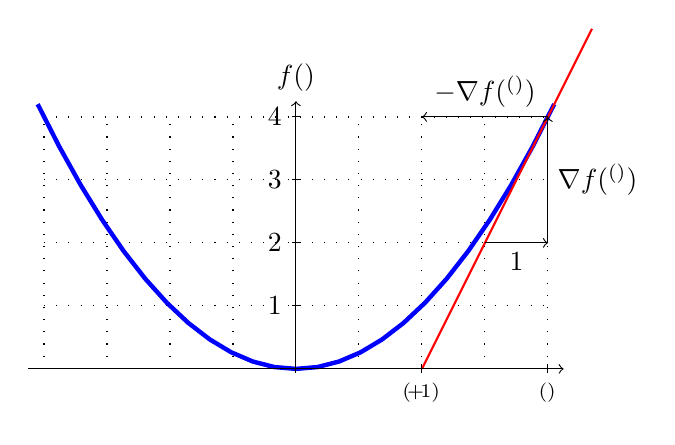
\begin{tikzpicture}[scale=0.8]
					\draw[loosely dotted] (-4,0) grid (4,4);
					\draw[blue, ultra thick, domain=-4.1:4.1] plot (\x,  {(1/4)*\x*\x});
					\draw[red, thick, domain=2:4.7] plot (\x,  {2*\x - 4});
					\draw[<-] (4,4) -- node[right] {$\nabla f(\weights^{(\itercntr)})$} (4,2);
					\draw[->] (4,4) -- node[above] {$-\lrate \nabla f(\weights^{(\itercntr)})$} (2,4);
					\draw[<-] (4,2) -- node[below] {$1$} (3,2) ;
					\draw[->] (-4.25,0) -- (4.25,0) node[right] {$\weights$};
					\draw[->] (0,-2pt) -- (0,4.25) node[above] {$f(\weights)$};
					\draw[shift={(0,0)}] (0pt,2pt) -- (0pt,-2pt) node[below] {$\overline{\weights}$};
					\draw[shift={(4,0)}] (0pt,2pt) -- (0pt,-2pt) node[below] {$\weights^{(\itercntr)}$};
					\draw[shift={(2,0)}] (0pt,2pt) -- (0pt,-2pt) node[below] {$\weights^{(\itercntr\!+\!1)}$};
					\foreach \y/\ytext in {1/1, 2/2, 3/3, 4/4}
					\draw[shift={(0,\y)}] (2pt,0pt) -- (-2pt,0pt) node[left] {$\ytext$};  
				\end{tikzpicture}
			\end{center}
			\caption{A single \gls{gradstep} \eqref{equ_def_GD_step_dict} towards the minimizer $\overline{\weights}$ of $f(\weights)$.}
			\label{fig_basic_GD_step_dict}
		\end{figure}
%		
		},first={gradient descent (GD)},text={GD}}

\newglossaryentry{abserr}{name={absolute error loss},description={
			Consider a \gls{datapoint} with \gls{feature}s $\featurevec \in \featurespace$ and numeric 
			\gls{label} $\truelabel \in \mathbb{R}$. The absolute error \gls{loss}\index{absolute error loss} 
			incurred by a \gls{hypothesis} $\hypothesis: \featurespace \rightarrow \mathbb{R}$ 
			is defined as $|\truelabel - \hypothesis(\featurevec)|$, i.e., the absolute difference between 
			the \gls{prediction} $\hypothesis(\featurevec)$ and the true \gls{label} $\truelabel$.},
	%		{\bf Example.} Imagine you are predicting the temperature for tomorrow. If the actual 
	%		temperature is 20 (measured in degree Celsius), but your model predicts 18, the absolute 
	%		error is $20−18=2$. This means your prediction was off by $2$ (degrees Celius). 
	%		The absolute error loss always gives a positive number, so it doesn't matter if the \gls{prediction} 
	%		is too high or too low - only the size of the difference matters.}
			first={absolute error loss},text={absolute error loss}}

\newglossaryentry{device}{name={device},description={
				Any\index{device} physical system that can be used to store 
				and process \gls{data}. In the context of \gls{ml}, 
				we typically mean a computer that is able to read in \glspl{datapoint} 
				from different sources and, in turn, to train an \gls{ml} \gls{model} 
				using these \glspl{datapoint}.},
				first={device},
				plural={devices},
				text={device}
			}

\newglossaryentry{llm}{name={large language model (LLM)},description={
	Large language \gls{model}s\index{large language model (LLM)} is an umbrella term for \gls{ml} methods 
	that process and generate human-like text. These methods typically 
	use \gls{deepnet}s with billions (or even trillions) of \gls{parameters}. 
	A widely used choice for the network architecture is referred to as 
	Transformers \cite{vaswani2017attention}. The training of large language \gls{model}s is often  
	based on the task of predicting a few words that are intentionally removed 
	from a large text corpus. Thus, we can construct \gls{labeled datapoint}s 
	simply by selecting some words of a text as \gls{label}s and the remaining 
	words as \gls{feature}s of \gls{datapoint}s. This construction requires 
	very little human supervision and allows for generating sufficiently 
	large \gls{trainset}s for large language \gls{model}s.},
					first={large language model (LLM)},text={LLM}}


\newglossaryentry{huberreg}{name={Huber regression},description={
			Huber \gls{regression}\index{Huber regression} refers to \gls{erm}-based methods 
			that use the \gls{huberloss} as a measure of the \gls{prediction} error. 
			Two important special cases of Huber \gls{regression} are \gls{ladregression} and 
			\gls{linreg}. Tuning the threshold parameter of the \gls{huberloss} allows the user
			to trade the robustness of the \gls{abserr} 
			against the computational benefits of the \gls{smooth} \gls{sqerrloss}.},
			first={Huber regression},text={Huber regression}}


\newglossaryentry{ladregression}{name={least absolute deviation regression},description={
		Least\index{least absolute deviation regression} absolute deviation regression is 
		an instance of \gls{erm} using the \gls{abserr}. It is a special case of 
		\gls{huberreg}.},
		first={least absolute deviation regression},text={least absolute deviation regression}}

%\newglossaryentry{metric}{name={metric},description={We\index{metric} sometimes use \emph{metric} to refer to 
%		a \gls{lthat is used solely 
%	    for the final performance evaluation of a learnt hypothesis. The metric is typically a \gls{lossfunc} that 
%	    has a ``natural'' interpretation (such as the \gls{zerooneloss}) but is not a good choice to guide 
%	    the learning process, e.g., via \gls{erm}. For \gls{erm}, we typically prefer \gls{lossfunc}s that depend smoothly 
%	    on the (parameters of the) hypothesis. Examples for such smooth \gls{lossfunc}s include the \gls{sqerrloss} 
%	    and the \gls{logloss} \eqref{equ_log_loss_gls}.},first={metric},text={metric}}

\newglossaryentry{bayesrisk}{name={Bayes risk},description={Consider a \gls{probmodel} with a 
joint \gls{probdist} $p(\featurevec,\truelabel)$ for the \gls{feature}s $\featurevec$ 
and \gls{label} $\truelabel$ of a \gls{datapoint}. The\index{Bayes risk} Bayes \gls{risk} 
is the \gls{minimum} possible \gls{risk} that can be achieved by any \gls{hypothesis} 
$\hypothesis: \featurespace \rightarrow \labelspace$. Any \gls{hypothesis} that achieves 
the Bayes risk is referred to as a \gls{bayesestimator} \cite{LC}.},first={Bayes risk},text={Bayes risk}}
	
\newglossaryentry{bayesestimator}{name={Bayes estimator},description={Consider\index{Bayes estimator} 
a \gls{probmodel} with a joint \gls{probdist} $p(\featurevec,\truelabel)$ for the \gls{feature}s $\featurevec$ and \gls{label} 
$\truelabel$ of a \gls{datapoint}. For a given \gls{lossfunc} $\lossfunc{\cdot}{\cdot}$, we refer to a \gls{hypothesis} 
$\hypothesis$ as a Bayes estimator if its \gls{risk} $\expect\{\lossfunc{\pair{\featurevec}{\truelabel}}{\hypothesis}\}$ is the 
\gls{minimum} \cite{LC}. Note that the property of a \gls{hypothesis} being a Bayes estimator depends on 
the underlying \gls{probdist} and the choice for the \gls{lossfunc} $\lossfunc{\cdot}{\cdot}$.},
		first={Bayes estimator},text={Bayes estimator}}


\newglossaryentry{weights}{name={weights},
	description={Consider\index{weights} a parametrized \gls{hypospace} $\hypospace$. 
		We\index{weights} use the term weights for numeric \gls{modelparams} that are 
		used to scale \gls{feature}s or their transformations in order to compute $\hypothesis^{(\weights)} \in \hypospace$. A \gls{linmodel} uses weights $\weights=\big(\weight_{1},\ldots,\weight_{\nrfeatures}\big)^{T}$ to compute 
		the linear combination $\hypothesis^{(\weights)}(\featurevec)= \weights^{T} \featurevec$. 
		Weights are also used in \gls{ann}s to form linear combinations of \gls{feature}s or the 
		outputs of neurons in hidden layers.},first={weights},text={weights}}
	
\newglossaryentry{probdist}{name={distribuzione di probabilità}, plural={distribuzioni di probabilità},
	description={Per\index{distribuzione di probabilità} analizzare i metodi di \gls{ml}, può essere utile 
		interpretare i \glspl{datapoint} come \glspl{realization} \gls{iid} di una \gls{rv}. Le proprietà 
		tipiche di tali \glspl{datapoint} sono quindi governate dalla distribuzione di \gls{probability}  
		di questa \gls{rv}. La distribuzione di \gls{probability} di una \gls{rv} binaria $\truelabel \in \{0,1\}$ 
		è determinata univocamente dalle probabilità $\prob{\truelabel = 0}$ e 
		$\prob{\truelabel=1}\!=\!1\!-\!\prob{\truelabel=0}$. La distribuzione di \gls{probability} 
		di una \gls{rv} a valori reali $\feature \in \mathbb{R}$ può essere definita tramite una 
		\gls{pdf} $p(\feature)$ tale che $\prob{ \feature \in [a,b] } \approx  p(a) |b-a|$. 
	    In generale, una distribuzione di \gls{probability} è definita da una misura di\cite{GrayProbBook}, \cite{BillingsleyProbMeasure}.
	    		\\
		Si veda anche: \gls{ml}, \gls{datapoint}, \gls{iid}, \gls{realization}, \gls{rv}, \gls{probability}, \gls{pdf}.},first={distribuzione di probabilità},text={distribuzione di probabilità}}
        
    
\newglossaryentry{pdf}
{name={probability density function (pdf)},
 description={The\index{probability density function (pdf)} pdf $p(\feature)$ of a real-valued \gls{rv} 
 	$\feature \in \mathbb{R}$ is a particular representation of its \gls{probdist}. If the pdf exists, it can 
 	be used to compute the \gls{probability} that $\feature$ takes on a value from a measurable set 
 	$\mathcal{B} \subseteq \mathbb{R}$ via $\prob{\feature \in \mathcal{B}} = \int_{\mathcal{B}} p(\feature') d \feature'$ \cite[Ch. 3]{BertsekasProb}. 
	If the pdf of a vector-valued \gls{rv} $\featurevec \in \mathbb{R}^{\featuredim}$ exists, it 
     allows us to compute the \gls{probability} of $\featurevec$ belonging to a measurable region $\mathcal{R}$ via 
        $\prob{\featurevec \in \mathcal{R}} = \int_{\mathcal{R}} p(\featurevec') d \feature_{1}' \ldots d \feature_{\featuredim}' $ \cite[Ch. 3]{BertsekasProb}.
        		\\
		See also: \gls{rv}, \gls{probdist}, \gls{probability}.},
first={probability density function (pdf)},
text={pdf}
}

\newglossaryentry{parameter}
{name={parametro},
	description={Il\index{parameter} parametro di un modello di \gls{ml} \gls{model} è una quantità regolabile (cioè apprendibile o 
	adattabile) che ci consente di selezionare tra diverse \glspl{map} \gls{hypothesis}. Ad esempio, il \gls{linmodel} $\hypospace \defeq \{\hypothesis^{(\weights)}: \hypothesis^{(\weights)}(\feature)= \weight_{1} \feature + \weight_{2}\}$ 
		consiste di tutte \glspl{map} \gls{hypothesis} $\hypothesis^{(\weights)}(\feature)= \weight_{1} \feature + \weight_{2}$ 
		con una particolare scelta dei parametri $\weights = \big(\weight_{1},\weight_{2}\big)^{T} \in \mathbb{R}^{2}$. 
		Un altro esempio di parametro di un \gls{model} è dato dai \gls{weights} assegnati a una connessione tra due neuroni di una \gls{ann}.
				\\
		Si veda anche: \gls{ml}, \gls{model}, \gls{hypothesis}, \gls{map}, \gls{linmodel}, \gls{weights}, \gls{ann}.},
		first={parametro},
		text={parametro},
		firstplural={parametri}, 
 		plural={parametri}
}

\newglossaryentry{lln}{name={law of large numbers},
	description={The\index{law of large numbers} law of large numbers refers to the 
		convergence of the average of an increasing (large) number of \gls{iid} \gls{rv}s 
		to the \gls{mean} of their common \gls{probdist}. Different instances of the 
		law of large numbers are obtained by using different notions of convergence \cite{papoulis}.},first={law of large numbers},text={law of large numbers}}
    
\newglossaryentry{stopcrit}
{name={stopping criterion},
	description={Many\index{stopping criterion} \gls{ml} methods use iterative \glspl{algorithm} 
		that construct a sequence of \gls{modelparams} in order to minimize the \gls{trainerr}. 
		For example, \gls{gdmethods} iteratively update the \glspl{parameter} of a parametric \gls{model}, 
		such as a \gls{linmodel} or a \gls{deepnet}. Given a finite amount of computational 
		resources, we need to stop updating the \glspl{parameter} after a finite number of iterations. 
		A stopping criterion is any well-defined condition for deciding when to stop  
		updating.
				\\
		See also: \gls{algorithm}, \gls{gdmethods}.},
		first={stopping criterion},
		firstplural={stopping criteria},
		plural={stopping criteria}, 
		text={stopping criterion}
}

\newglossaryentry{kCV}{name={$k$-fold cross-validation ($\nrfolds$-fold CV)},
	description={$k$-fold CV\index{$k$-fold cross-validation ($\nrfolds$-fold CV)} is a 
		method for learning and validating a \gls{hypothesis} using a given \gls{dataset}. 
		This method divides the \gls{dataset} evenly into $k$ subsets or folds 
		and then executes $k$ repetitions of \gls{model} training (e.g., via \gls{erm}) and \gls{validation}. 
		Each repetition uses a different fold as the \gls{valset} and the remaining $k-1$ folds 
		as a \gls{trainset}. The final output is the average of the \gls{valerr}s obtained 
		from the $k$ repetitions.},first={$k$-fold cross-validation ($k$-fold CV)},text={$k$-fold CV}}
	
\newglossaryentry{renyidiv}{name={R\'enyi divergence}, 
	sort={Renyi},
	description={The R\'enyi divergence\index{R\'enyi divergence} measures the (dis)similarity 
		between two \gls{probdist}s \cite{RenyiInfo95}.}, 
	first = {R\'enyi divergence}, text = {R\'enyi divergence}} 

\newglossaryentry{nonsmooth}{name={non-smooth},
	description={We\index{non-smooth} refer to a function as non-smooth if it is not 
		\gls{smooth} \cite{nesterov04}.},first={non-smooth},text={non-smooth}}

\newglossaryentry{convex}{name={convex},
	description={A\index{convex} subset $\mathcal{C} \subseteq \mathbb{R}^{\featuredim}$ of the 
		\gls{euclidspace} $\mathbb{R}^{\featuredim}$ is referred to as convex if it contains 
		the line segment between any two points $\vx, \vy\!\in\!\cluster$ in that set. A function 
		$f\!:\!\mathbb{R}^{\dimlocalmodel}\!\rightarrow\!\mathbb{R}$ 
		is convex if its epigraph $\big\{ \big( \weights^{T},t \big)^{T}\!\in\!\mathbb{R}^{\dimlocalmodel\!+\!1}\!:\!t\!\geq\!f(\weights) \}$ 
		is a convex set \cite{BoydConvexBook}. We illustrate one example of a convex set 
		and a convex function in Figure \ref{fig_convex_set_function}. 
		\begin{figure}[H]
		\begin{center}
			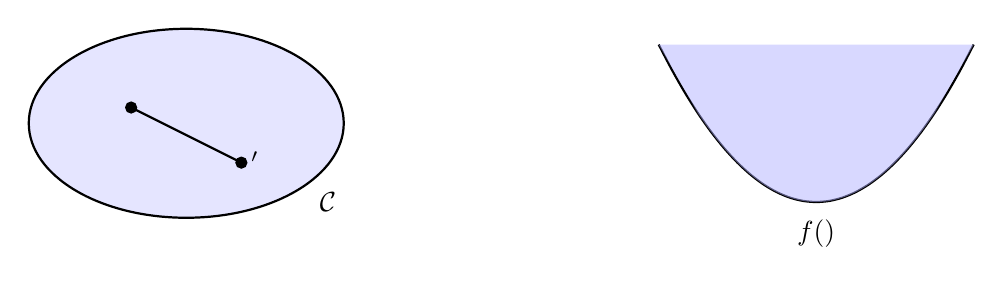
\begin{tikzpicture}
				% Left part: Convex set (Ellipse)
				\fill[blue!20, opacity=0.5] (-3,0) ellipse (2 and 1.2); % Shaded ellipse
				\draw[thick] (-3,0) ellipse (2 and 1.2);
			 % Points inside the ellipse
				\filldraw[black] (-3.7,0.2) circle (2pt) node[left] {$\vw$};
				\filldraw[black] (-2.3,-0.5) circle (2pt) node[right] {$\vw'$};
				% Line segment connecting the two points
				\draw[thick] (-3.7,0.2) -- (-2.3,-0.5);
				% Label for the convex set
				\node at (-1.2,-1.0) {$\mathcal{C}$};
				% Right part: Convex function and epigraph
				\begin{scope}[shift={(5,-1)}]
					% Define the convex function
					\draw[thick, domain=-2:2, smooth, variable=\x] 
					plot ({\x}, {0.5*\x*\x});
					% Shaded epigraph (area above the function)
					\fill[blue!30, opacity=0.5] 
					plot[domain=-1.5:1.5, smooth] ({\x}, {0.5*\x*\x}) -- 
					(2, {0.5*2*2}) -- 
					(-2, {0.5*2*2}) -- 
					cycle;
					%\fill[blue!30, opacity=0.5] (-1.5,1.2) -- (-1.5,2.5) -- (1.5,2.5) -- (1.5,1.2) -- plot[domain=-1.5:1.5, smooth] ({\x}, {0.5*\x*\x}) -- cycle;
					% Labels
					\node at (0,-0.4) {$f(\weights)$};
				\end{scope}
			\end{tikzpicture}
			\vspace*{-8mm}
			\end{center}
			\caption{Left: A convex set $\cluster \subseteq \mathbb{R}^{\dimlocalmodel}$. 
				Right: A convex function $f: \mathbb{R}^{\dimlocalmodel} \rightarrow \mathbb{R}$.\label{fig_convex_set_function}}
		\end{figure}},first={convex},text={convex}}


\newglossaryentry{smooth}{name={smooth},
	description={A\index{smooth} real-valued function $f: \mathbb{R}^{\dimlocalmodel} \rightarrow \mathbb{R}$ 
		is smooth if it is \gls{differentiable} and its \gls{gradient} $\nabla f(\weights)$ is continuous at all $\weights \in \mathbb{R}^{\dimlocalmodel}$  \cite{nesterov04,CvxBubeck2015}. A smooth function $f$ is referred to as $\beta$-smooth if the \gls{gradient} 
		$\nabla f(\weights)$ is Lipschitz continuous with Lipschitz constant $\beta$, i.e., 
		$$\| \nabla f(\weights) - \nabla f(\weights') \| \leq \beta \| \weights - \weights' \| \mbox{, for any } \weights,\weights' \in \mathbb{R}^{\dimlocalmodel}.$$ 
		The constant $\beta$ quantifies the amount of smoothness of the function $f$: the smaller the $\beta$, 
		the smoother $f$ is. Optimization problems with a smooth \gls{objfunc} can be solved effectively by \gls{gdmethods}. 
	    Indeed, \gls{gdmethods} approximate the \gls{objfunc} locally around a current choice $\weights$ 
	    using its \gls{gradient}. This approximation works well if the \gls{gradient} does 
	    not change too rapidly. We can make this informal claim precise by studying the effect of a single 
	    \gls{gradstep} with \gls{stepsize} $\lrate=1/\beta$ (see Figure \ref{fig_gd_smooth_dict}). 
	    \begin{figure}[H] 
	    	\begin{center} 
	    	\begin{tikzpicture}[scale=0.8, x=0.7cm,y=0.05cm]
	    		% Parameter to shift the quadratic curve horizontally
	    		\def\hshift{0.5} % Change this value to shift the curve horizontally
	    		% Define the function (only the increasing part of x^2 for x >= 0)
	    		\draw[thick, domain=\hshift:8+\hshift, smooth, variable=\x] plot ({\x}, {\x^2}); %node[right] {$f(x) = x^2$};
	    		% Define points for the tangents
	    		\coordinate (w) at (\hshift,{\hshift*\hshift}); % Point w on the curve (left end of the plot)
	    		\coordinate (wkplus1) at (4+\hshift,{(4+\hshift)^2}); % Point w^{k+1} on the curve (x=1 + hshift, y=1)
	    		\coordinate (wk) at (8+\hshift,{(8+\hshift)^2}); % Point w^k on the curve (right end of the plot)
	    		% Calculate the slopes for the tangents
  				\draw[line width=1pt, transform canvas={yshift=-2pt}] (wk) -- +(-1, -{2*(8 + \hshift)} ) -- +(1, {2*(8 + \hshift)}); % Tangent at w^k with positive slope
 				\draw[line width=1pt, transform canvas={yshift=-2pt}] (w) -- +(-1, -{2*\hshift} ) -- +(1, {2*\hshift} )  node[below] {$\nabla f(\weights)$};% Tangent at w with slope 0 (since derivative at hshift = 0)
%	    		% Draw filled circles at points w^k, w, and w^{k+1}
	    		\filldraw (wk) circle (2pt) node[above left] {$\weights^{(\iteridx)}$} node[below right] {$\nabla f(\weights^{(\iteridx)})$} ;
	    		\filldraw (w) circle (2pt) node[above right] {$\weights$} ;
	    		\filldraw (wkplus1) circle (2pt) node[below right] {$\weights^{(\iteridx+1)}\!=\!\weights^{(\iteridx)}\!-\!(1/\beta)\nabla f(\weights^{(\iteridx)})$};
	    		    % Draw horizontal rulers to mark the function values at wk and wk_plus1
	    		\draw[dashed] (wk) -- ($(8,0) + (wk)$) ; %node[left] {$f(\weights^{(\iteridx)})$};
	    		\draw[dashed] (wkplus1) -- ($(12,0) + (wkplus1)$) ; %node[left] {$f(\weights^{(\iteridx+1)})$};
	    		 \draw[<->, thick] ($(4,0) + (wk)$) -- ($(8,0) + (wkplus1)$) 
	    		node[midway, right] {$ f\big(\weights^{(\iteridx)}\big)\!-\!f\big(\weights^{(\iteridx+1)}\big)\!\geq\!\frac{1}{2\beta}\normgeneric{\nabla f(\weights^{(\iteridx)})}{2}^{2}$};
%	    		% Label the curve
%	    		\node at (2, 4) {};
	    	\end{tikzpicture}
	    	\end{center}
	    	\caption{Consider an \gls{objfunc} $f(\weights)$ that is $\beta$-smooth. 
	    		Taking a \gls{gradstep}, with \gls{stepsize} $\lrate = 1/\beta$, decreases the 
	    		objective by at least $\frac{1}{2\beta}\normgeneric{\nabla f(\weights^{(\iteridx)})}{2}^{2}$ \cite{nesterov04,CvxAlgBertsekas,CvxBubeck2015}. 
	    		Note that the \gls{stepsize} $\lrate = 1/\beta$ becomes larger for smaller $\beta$. Thus, 
	    		for smoother \gls{objfunc}s (i.e., those with smaller $\beta$), 
				we can take larger steps. \label{fig_gd_smooth_dict}}
	    	\end{figure}
	    },first={smooth},text={smooth}}

\newglossaryentry{paramspace}{name={parameter space},
		description={The\index{parameter space} parameter space $\paramspace$ of 
		an \gls{ml} \gls{model} $\hypospace$ is the set of all feasible choices for the 
		\gls{modelparams} (see Figure \ref{fig_param_space_dict}). Many important \gls{ml} methods 
		use a \gls{model} that is parametrized by vectors of the \gls{euclidspace} $\mathbb{R}^{\dimlocalmodel}$. 
		Two widely used examples of parametrized \gls{model}s are \gls{linmodel}s 
		and \gls{deepnet}s. The parameter space is then often a subset $\paramspace \subseteq \mathbb{R}^{\dimlocalmodel}$, 
		e.g., all vectors $\weights \in \mathbb{R}^{\dimlocalmodel}$ with a \gls{norm} smaller than one.
		\begin{figure}[H]
			\begin{center}
			\begin{tikzpicture}
				% Left part: Ellipse representing parameter space (with two dots)
				\node[ellipse, minimum width=3cm, minimum height=2cm, draw, thick] (paramspace) {};
				\node[below=0.1cm of paramspace] {parameter space $\paramspace$};
				% Two dots inside the left ellipse
				\node[black, circle, inner sep=2pt, fill] (theta1) at ($(paramspace.north west) + (1, -1)$) {};
				\node[left=0.01cm of theta1] {$\weights$};
				\node[black, circle, inner sep=2pt, fill] (theta2) at ($(paramspace.south east) + (-1.5, 1)$) {};
				\node[left=0.01cm of theta2] {$\weights'$};
				% Right part: Ellipse containing two smaller plots
				\node[ellipse, minimum width=7cm, minimum height=3cm, draw, thick, right=4cm of paramspace] (plotcloud) {};
				\node[above=0.2cm of plotcloud] {\gls{model} $\hypospace$};
				% Axis for first smaller plot
				\node (plot1start) at ($(plotcloud.south west) + (0.2, 0.2)$) {};
				%\draw[thick, ->] (plot1start) -- ++(2, 0) node[anchor=north] {$\featurevec$};
				%\draw[thick, ->] (plot1start) -- ++(0, 1.5) node[anchor=east] {$\truelabel$};
				% Simple plot line in first smaller plot
				\draw[thick, red] (plot1start) .. controls ++(0.8, 1) and ++(-0.8, -0.8) .. ($(plotcloud.south west) + (2.8, 0.8)$) node[anchor=west] {$\hypothesis^{(\weights)}$};
				% Axis for second smaller plot
				\node (plot2start) at ($(plotcloud.south west) + (1.0, 1.2)$) {};
			%	\draw[thick, ->] (plot2start) -- ++(2, 0) node[anchor=north] {$\featurevec$};
			%	\draw[thick, ->] (plot2start) -- ++(0, 1.5) node[anchor=east] {$\truelabel$};
				% Simple plot line in second smaller plot
				\draw[thick, blue] (plot2start) .. controls ++(0.8, 0.5) and ++(-0.8, -0.8) .. ($(plotcloud.south west) + (2.8, 2.1)$) node[anchor=west] {$\hypothesis^{(\weights')}$};
				% Connect the two dots in the parameter space to the two plots
				\draw[thick, ->, bend right=20] (theta1) to ($(plot1start) + (0,0)$);
				\draw[thick, ->, bend left=20] (theta2) to (plot2start);
			\end{tikzpicture}
			\end{center} 
			\caption{The parameter space $\paramspace$ of an \gls{ml} \gls{model} $\hypospace$ consists of all 
			feasible choices for the \gls{modelparams}. Each choice $\weights$ for the \gls{modelparams} 
			selects a \gls{hypothesis} map $\hypothesis^{(\weights)} \in \hypospace$.
				 \label{fig_param_space_dict}} 
\end{figure}},
			first={parameter space},text={parameter space}}

\newglossaryentry{datanorm}{name={data normalization},
	description={\Gls{data} normalization\index{data normalization} refers to transformations 
		applied to the \gls{featurevec}s of \gls{datapoint}s to improve the \gls{ml} method's 
		\gls{statasp} or \gls{compasp}. For example, in \gls{linreg} with \gls{gdmethods} using 
		a fixed \gls{learnrate}, convergence depends on controlling the \gls{norm} of \gls{featurevec}s 
		in the \gls{trainset}. A common approach is to normalize \gls{featurevec}s such that their 
		\gls{norm} does not exceed one \cite[Ch.\ 5]{MLBasics}.},
	first={data normalization},text={data normalization}}

\newglossaryentry{dataaug}{name={data augmentation},
	description={\Gls{data} augmentation\index{data augmentation} methods add synthetic \gls{datapoint}s 
		to an existing set of \gls{datapoint}s. These synthetic \gls{datapoint}s are obtained by 
		perturbations (e.g., adding noise to physical measurements) or transformations 
		(e.g., rotations of images) of the original \gls{datapoint}s. These perturbations and 
		transformations are such that the resulting synthetic \gls{datapoint}s should 
		still have the same \gls{label}. As a case in point, a rotated cat image is still 
		a cat image even if their \gls{featurevec}s (obtained by stacking pixel color intensities) 
		are very different (see Figure \ref{fig_symmetry_dataaug_dict}). \Gls{data} augmentation can be an 
		efficient form of \gls{regularization}.
		\begin{figure}[H]
		\begin{center}
			\begin{tikzpicture}
				% Define shift macros locally
				\newcommand{\xshift}{0.5}
				\newcommand{\yshift}{2}
				% Define the shifted curves
				% Define the shifted curves
  				\draw[very thick, blue] plot[smooth, tension=1] coordinates {(0,0) (2,1) (4,0) (6,-1) (8,0)};
  				\node[blue, right] at (0,0) {\textbf{cat}};
  				\draw[very thick, red, dashed] plot[smooth, tension=1] coordinates {(0 + \xshift,0 + \yshift) (2 + \xshift,1 + \yshift) (4 + \xshift,0 + \yshift) (6 + \xshift,-1 + \yshift) (8 + \xshift,0 + \yshift)};
  				\node[red, right] at (8 + \xshift,0 + \yshift) {\textbf{no cat}};
				\fill[blue] (2,1) circle (2pt) node[above] {$\featurevec^{(1)}$};
				\fill[blue] (6,-1) circle (2pt) node[above] {$\featurevec^{(2)}$};
				  % Draw a bent arrow connecting the two points with custom in and out angles
				  \draw[->, thin, >=latex, line width=0.5pt] (2,1) to[out=240, in=240] node[midway, below] {$\mathcal{T}^{(\eta)}$} (6,-1);
			  \end{tikzpicture}
			  \vspace*{-11mm}
		\end{center}
		\caption{\Gls{data} augmentation exploits intrinsic symmetries of \gls{datapoint}s in 
		       some \gls{featurespace} $\featurespace$. We can represent a symmetry by 
		     an operator $\mathcal{T}^{(\eta)}: \featurespace \rightarrow \featurespace$,
		     parametrized by some number $\eta \in \mathbb{R}$. For example, $\mathcal{T}^{(\eta)}$ 
		    might represent the effect of rotating a cat image by $\eta$ degrees. A \gls{datapoint} 
		    with \gls{featurevec} $\featurevec^{(2)} = \mathcal{T}^{(\eta)} \big(\featurevec^{(1)} \big)$ must 
		    have the same \gls{label} $\truelabel^{(2)}=\truelabel^{(1)}$ as a \gls{datapoint} 
		     with \gls{featurevec} $\featurevec^{(1)}$.\label{fig_symmetry_dataaug_dict}}
		 \end{figure} },first={data augmentation},text={data augmentation}}
	
	
\newglossaryentry{localdataset}{name={local dataset},description={The\index{local dataset} concept of a local \gls{dataset} is 
		in between the concept of a \gls{datapoint} and a \gls{dataset}. A local \gls{dataset} consists of several 
		individual \gls{datapoint}s, which are characterized by \gls{feature}s and \gls{label}s. 
		In contrast to a single \gls{dataset} used in basic \gls{ml} methods, a local \gls{dataset} is also 
		related to other local \gls{dataset}s via different notions of similarity. These similarities 
		might arise from \gls{probmodel}s or communication infrastructure and 
		are encoded in the edges of an \gls{empgraph}.},first={local dataset},text={local dataset}}
	
\newglossaryentry{localmodel}{name={local model},description={Consider\index{local model} a collection 
		of \gls{localdataset}s that are assigned to the nodes of an \gls{empgraph}. A local \gls{model} $\localmodel{\nodeidx}$ 
		is a \gls{hypospace} assigned to a node $\nodeidx \in \nodes$. Different nodes might be assigned 
		different \gls{hypospace}s, i.e., in general $\localmodel{\nodeidx} \neq \localmodel{\nodeidx'}$ for different 
		nodes $\nodeidx, \nodeidx' \in \nodes$.  },first={local model},text={local model}}
	
\newglossaryentry{mutualinformation}
{name={mutual information (MI)},
 description={The\index{mutual information (MI)} MI $\mutualinformation{\featurevec}{\truelabel}$ 
 	between two \gls{rv}s $\featurevec$, $\truelabel$ defined on the same \gls{probspace} 
 	is given by \cite{coverthomas} $$\mutualinformation{\featurevec}{\truelabel} \defeq 
	\expect \left\{ \log \frac{p (\featurevec,\truelabel)}{p(\featurevec)p(\truelabel)} \right\}.$$ 
	It is a measure of how well we can estimate $\truelabel$ based 
	solely on $\featurevec$. A large value of $\mutualinformation{\featurevec}{\truelabel}$ indicates that 
	$\truelabel$ can be well predicted solely from $\featurevec$. This \gls{prediction} could be obtained by a 
		\gls{hypothesis} learned by an \gls{erm}-based \gls{ml} method. 
	 }, first={MI}, text={MI} 
}

\newglossaryentry{zerogradientcondition}{name={zero-gradient condition},
	description={Consider\index{zero-gradient condition} the unconstrained 
		optimization problem $\min_{\weights \in \mathbb{R}^{\dimlocalmodel}} f(\weights)$  with 
			a \gls{smooth} and \gls{convex} \gls{objfunc} $f(\weights)$. A necessary and 
			sufficient condition for a vector $\widehat{\weights} \in \mathbb{R}^{\dimlocalmodel}$ 
			to solve this problem is that the \gls{gradient} $\nabla f \big( \widehat{\weights} \big)$ 
			is the zero vector, 
			$$ \nabla f \big( \widehat{\weights} \big) = \mathbf{0} \Leftrightarrow  f \big( \widehat{\weights} \big) = \min_{\weights \in \mathbb{R}^{\dimlocalmodel}} f(\weights) .$$ }, 
			first={zero-gradient condition},text={zero-gradient condition}}


\newglossaryentry{edgeweight}{name={edge weight},
	description={Each\index{edge weight} edge $\edge{\nodeidx}{\nodeidx'}$ of an \gls{empgraph} is 
		assigned a non-negative edge weight $\edgeweight_{\nodeidx,\nodeidx'}\geq0$. 
		A zero edge weight $\edgeweight_{\nodeidx,\nodeidx'}=0$ indicates the absence 
		of an edge between nodes $\nodeidx, \nodeidx' \in \nodes$.}, 
	first={edge weight},text={edge weight}}


\newglossaryentry{dataminprinc}{name={data minimization principle},
	description={European\index{data minimization principle} \gls{data} protection regulation 
		includes a \gls{data} minimization principle. This principle requires a \gls{data} controller to 
		limit the collection of personal information to what is directly relevant and necessary 
		to accomplish a specified purpose. The \gls{data} should be retained only for as long as 
		necessary to fulfill that purpose \cite[Article 5(1)(c)]{GDPR2016}, \cite{EURegulation2018}.}, 
	first={data minimization principle},text={data minimization principle}}


